% Template LaTeX Tesis Ciencia de la Computación UCSP
% 2022

\documentclass[a4paper,openany,12pt]{book}
\usepackage[utf8]{inputenc}
\usepackage{graphicx}
\usepackage[spanish,mexico]{babel}
\usepackage{sty/fancyhdr}
\usepackage{ae}
\usepackage[left=2.5cm,right=2.5cm,top=3cm,bottom=2cm]{geometry}
\usepackage[printonlyused]{acronym}
\usepackage{xspace}
\usepackage{sty/hlundef}
\usepackage{sty/tesis}
\usepackage{setspace}
\usepackage{booktabs}
\usepackage{array}
\usepackage{amssymb}
\usepackage{amsmath}
\usepackage{amsthm}
\usepackage{algorithm}
\usepackage{algpseudocode}
\usepackage{tikz}
\usetikzlibrary{babel,positioning,arrows.meta,shapes.geometric,patterns}

% Entornos de teoremas (numerados por capítulo)
\newtheorem{proposicion}{Proposición}[chapter]
\newtheorem{corolario}{Corolario}[chapter]
\theoremstyle{definition}
\newtheorem{definicion}{Definición}[chapter]
\theoremstyle{remark}
\newtheorem{observacion}{Observación}[chapter]
\theoremstyle{plain}

% Pseudocódigo en español
\floatname{algorithm}{Algoritmo}
\renewcommand{\listalgorithmname}{Lista de algoritmos}
\algrenewcommand\algorithmicrequire{\textbf{Entrada:}}
\algrenewcommand\algorithmicensure{\textbf{Salida:}}
\algrenewcommand\algorithmicif{\textbf{si}}
\algrenewcommand\algorithmicthen{\textbf{entonces}}
\algrenewcommand\algorithmicelse{\textbf{si no}}
\algrenewcommand\algorithmicfor{\textbf{para}}
\algrenewcommand\algorithmicforall{\textbf{para cada}}
\algrenewcommand\algorithmicdo{\textbf{hacer}}
\algrenewcommand\algorithmicreturn{\textbf{devolver}}
\algrenewcommand\algorithmicfunction{\textbf{función}}
\algrenewcommand\algorithmicprocedure{\textbf{procedimiento}}
\algrenewcommand\algorithmicend{\textbf{fin}}

\title{Extensión de ST-CC con refinamiento jerárquico por bloques para la detección de patrones
espacio-temporales locales}

\author{Luis Fabian Diaz Alvizuri}


\advisor{Dr. Erick Mauricio Gómez Nieto}


\date{Arequipa, Mes Año}

%\examinerone{Prof. Dr. Hidalgo Buena Gente}{Presidente}%
%\examinertwo{Prof. Dr. Antero A. Gal Oppe}{Secretario}%
%\examinerthree{Prof. Dr. Liu Xiao Ling}{University of ...} % of being the case

\dedicado{Aquí deberás colocar a quien va dedicada tu tesis por ejemplo: A Dios, por todo lo que me ha dado, a todos los profesores por sus enseñanzas y algunos amigos.}

\begin{document}
\pagestyle{fancy}

\maketitle %Compone la carátula y la dedicatoria
\newpage

%\approved{\tres}%  {\tres} or {\cuatro}

%mayores detalles de como usas las abreviaturas (acronimos)
% vea: http://www.ctan.org/tex-archive/macros/latex/contrib/acronym/
% hay un manual en pdf en esa misma direccion

\chapter*{Abreviaturas}

\begin{acronym}
% Añadir estas entradas dentro del entorno acronym de abreviaturas.tex
\acro{CC}{Co-agrupamiento (\emph{Co-Clustering})}
\acro{ST-CC}{\emph{Spatio-Temporal Co-Clustering}}
\acro{BBACI}[BBAC\_I]{\emph{Bregman Block Average Co-clustering} con I-divergencia}
\acro{AST-CC}{\emph{Adaptive Spatio-Temporal Co-Clustering}}
\end{acronym}


\begin{agradecimientos}
Aquí deberás colocar a quien y porque agradeces. Ejemplo:

En primer lugar deseo agradecer a Dios por haberme guiado a lo largo de estos cinco años de estudio.

Agradezco a mis padres por el apoyo brindado para forjarme como un profesional.

Agradezco a la universidad, mi \textit{alma matter}, por haberme cobijado y brindado la formación que ahora me permitirá ayudar a construir una mejor sociedad.

Agradezco de forma muy especial a mi asesor Prof. Dr./Mag. nombre 1 por haberme guiado en esta tesis. ...

Deseo agradecer de forma especial a mis profesores: nombre 1, nombre 2, nombre 3 porque fueron ejemplos que deseo seguir en mi vida profesional.

Deseo agradecer al personal administrativo de la universidad: nombre 1, nombre 2, nombre 3. Muchas gracias por la atención brindada y porque siempre estuvieron dispuestas a ayudarnos.
\end{agradecimientos}
 %Inserta los agradecimientos
\begin{resumen}
Aquí deberás colocar hasta 300 palabras como máximo, describiendo el problema que intentas resolver, la justificación, aportes o soluciones que planteas, qué tanto los haz alcanzado en calidad de resultados obtenidos.
\end{resumen}
 %Inserta el resumen
\begin{abstract}
Here you should enter up to 300 words maximum, describing the problem you are trying to solve, the justification, contributions or solutions you are proposing, how much you have achieved them in terms of obtained outcomes.
\end{abstract}
 %Inserta el abstract

\pagenumbering{roman}
\setcounter{page}{1}
\pagestyle{plain}

\tableofcontents %Inserta el índice general
\listoftables %Inserta el índice de cuadros
\listoffigures %Inserta el índice de figuras

%%%%%%%%%%%%%%%%%%%%%%%%%%%%%%%%%%%%%%%%%%%%%%%%%%%%%%%%%%%%%%%%%%%%%
%%%%   En esta parte deberas incluir los archivos de tu tesis   %%%%%
%%%%%%%%%%%%%%%%%%%%%%%%%%%%%%%%%%%%%%%%%%%%%%%%%%%%%%%%%%%%%%%%%%%%%

\pagestyle{plain}
\pagenumbering{arabic}
\setcounter{page}{1}
% =====================================================================
% Capítulo 1 - Introducción
% Tesis: Extensión de ST-CC con refinamiento jerárquico por bloques
%        para la detección de patrones espacio-temporales locales
% =====================================================================

\chapter{Introducción}
\label{chap:introduccion}

El presente capítulo introduce el problema abordado en esta tesis. Se parte
del contexto general del análisis de datos espacio-temporales, se describe
la limitación específica del co-agrupamiento de rejilla regular que motiva
el trabajo, y se presentan los objetivos, la organización del documento y
el cronograma de actividades.

% ---------------------------------------------------------------------
\section{Motivación y Contexto}
\label{sec:motivacion}

El avance de los sensores, los dispositivos con posicionamiento global y
los sistemas de registro automático ha hecho que grandes volúmenes de datos
espacio-temporales estén disponibles de forma cotidiana. Los registros de
viajes en taxi, los catálogos sísmicos o las series de monitoreo ambiental
describen dónde y cuándo ocurre un fenómeno, y su análisis
permite comprender la dinámica de una ciudad o de un territorio y apoyar la
toma de decisiones en planificación urbana, transporte y gestión de riesgos
\cite{Liu2021}.

Sin embargo, estos datos presentan una dificultad característica, y es que la
dimensión espacial y la temporal no son independientes. En la movilidad
urbana, por ejemplo, los destinos de los viajes se concentran en zonas de
trabajo durante la mañana y en zonas residenciales durante la tarde. Un
patrón de este tipo solo es visible si se observan ambas dimensiones a la
vez. Las técnicas tradicionales de agrupamiento espacio-temporal suelen
analizar una sola dimensión, o bien tratan cada dimensión por separado, lo
cual puede producir resultados poco representativos y perder la información
de interacción entre espacio y tiempo \cite{Liu2021}.

El \ac{CC} ofrece una alternativa natural a este problema. En lugar de
agrupar solo filas o solo columnas, particiona simultáneamente ambas
dimensiones de una matriz de datos. Aplicado a una matriz de co-ocurrencia
$O \in \mathbb{R}_{+}^{m \times n}$, cuyas filas son regiones y cuyas
columnas son intervalos de tiempo, el co-agrupamiento identifica grupos de
regiones que se comportan de manera similar en ciertos grupos de horarios.
Sobre esta idea, \cite{Liu2021} propusieron el marco \ac{ST-CC}, que emplea
el algoritmo \ac{BBACI} \cite{Banerjee2007} para descubrir patrones de
movilidad en los datos de taxis de Manhattan. Su estudio utilizó alrededor
de diez millones de viajes registrados en noviembre de 2017, agregados en
66 regiones y 12 intervalos de dos horas.

El resultado de \ac{BBACI} es una partición en tablero de ajedrez
(\emph{checkerboard}) donde cada región pertenece a un único grupo de regiones y
cada intervalo a un único grupo temporal, de modo que la matriz queda
dividida en $K_R \times K_T$ bloques rectangulares. Esta estructura es
fácil de interpretar, pero es global. Si una subzona de un grupo de
regiones se comporta de manera distinta solo en un horario concreto, por
ejemplo un foco de actividad alrededor de una estación de trenes al final
de la tarde, la única forma de capturarlo es dividir el grupo de regiones
completo en todos los horarios. En otras palabras, un detalle local obliga
a aumentar la resolución de toda la fila o columna de la partición. Este
problema también fue señalado en la literatura de modelos de bloques, donde
motivó enfoques bayesianos no paramétricos como el proceso de Mondrian
\cite{Roy2008}.

\cite{Liu2021} reconocieron parte de esta limitación y aplicaron
K-means sobre los bloques del tablero para obtener \emph{co-clusters} que no
siguen la rejilla. No obstante, ese paso reagrupa bloques ya
existentes a partir de su media y desviación estándar; no subdivide
un bloque internamente. Por tanto, la heterogeneidad que queda oculta dentro
de un bloque, que es precisamente donde pueden residir los patrones locales,
no se recupera. La alternativa de aumentar $K_R$ y $K_T$, o de elegirlos
automáticamente con métodos como Cross-Associations \cite{Chakrabarti2004},
sigue produciendo una rejilla global y aumenta el número de parámetros en
toda la matriz.

Una segunda pregunta surge al intentar refinar localmente, ¿cuándo debería detenerse?
Todo bloque presenta algo de variación, de modo que se necesita un criterio
que distinga la heterogeneidad real del ruido. Dos rasgos de los datos de
movilidad hacen que esa distinción no sea trivial. El primero es que la matriz
agrega varios días, y la actividad de cada celda varía de un día a otro mucho
más de lo que supone el modelo de Poisson, y de forma correlacionada entre
celdas, porque factores como el clima afectan a muchas regiones a la vez; una
prueba que ignore esa variabilidad declara heterogéneo casi cualquier bloque. El
segundo es que, con millones de viajes, incluso una diferencia irrelevante
resulta estadísticamente significativa. En agrupamiento interpretable
basado en árboles, \cite{Hu2025} propusieron evaluar cada división candidata
mediante pruebas de hipótesis, elegir la de menor $p$-valor y detener el
crecimiento cuando ninguna división es estadísticamente significativa. Este
principio, sin embargo, fue desarrollado para agrupar datos categóricos en
una sola dimensión y no para bloques bidimensionales de una matriz
espacio-temporal.

Esta tesis se sitúa en la intersección de ambas líneas. Se propone extender
\ac{ST-CC} con un refinamiento jerárquico que actúe dentro de cada
bloque, guiado por un criterio estadístico coherente con la misma función
objetivo que optimiza \ac{BBACI}. En el caso de conteos, la I-divergencia
que minimiza \ac{BBACI} coincide, salvo un factor constante, con la
devianza de un modelo log-lineal de Poisson. En consecuencia, la reducción
de divergencia al partir un bloque puede interpretarse como un estadístico
de razón de verosimilitud. Esta conexión permite construir el criterio de
refinamiento a partir del propio marco de \ac{ST-CC}, en lugar de importar
un criterio ajeno. Para que el criterio sea fiable, su distribución de
referencia se obtiene remuestreando los días que forman la matriz, de modo que
refleje la variabilidad real de los datos y no la que supondría un modelo de
Poisson, y la decisión de refinar exige, además de significancia, un tamaño de
efecto mínimo. El resultado puede aplicarse en otros dominios con datos de
conteo espacio-temporales agregados a partir de réplicas, como días o semanas.

% ---------------------------------------------------------------------
\section{Planteamiento del Problema}
\label{sec:problema}

El marco \ac{ST-CC} impone una partición en rejilla regular sobre la matriz
región~$\times$~tiempo, en la que cada división de filas o columnas se
aplica a la matriz completa. Como consecuencia, los patrones
espacio-temporales locales, es decir, la interacción entre un
subconjunto de regiones y un subconjunto de horarios que ocurre solo dentro
de un bloque, quedan promediados y ocultos, y la única manera de revelarlos
es aumentar la resolución global a costa de fragmentar innecesariamente el
resto de la matriz. Además, no existe un criterio estadístico que indique
si un bloque contiene heterogeneidad real que justifique subdividirlo, ni
que controle el riesgo de producir refinamientos espurios cuando se evalúan
muchas divisiones candidatas sobre los mismos datos. Ese criterio debe tener
en cuenta que la matriz es la suma de varios días cuya variabilidad excede la
de un modelo de Poisson, y que con millones de viajes la significancia
estadística no basta para distinguir un patrón relevante. El problema que aborda
esta tesis es, por tanto, cómo refinar localmente y de forma
estadísticamente justificada la partición de \ac{ST-CC} para detectar
patrones espacio-temporales locales, manteniendo la interpretabilidad del
resultado.

% ---------------------------------------------------------------------
\section{Objetivos}
\label{sec:objetivos}

El objetivo general de esta tesis es proponer y validar una extensión de
\ac{ST-CC} basada en un refinamiento jerárquico por bloques, que se aplique
sobre la partición en tablero que produce el marco original y que esté guiado
por pruebas de significancia estadística derivadas de la I-divergencia. Se
busca que esta extensión permita detectar patrones espacio-temporales locales,
es decir, la interacción entre un subconjunto de regiones y un subconjunto de
horarios que ocurre solo dentro de un bloque y que la partición en rejilla
regular no captura. Al mismo tiempo, se espera que el criterio con el que se
decide cada refinamiento sea coherente con la función objetivo del
co-agrupamiento, que distinga la heterogeneidad real del ruido y que preserve
la interpretabilidad del resultado, de modo que los patrones locales
detectados puedan leerse directamente como grupos de regiones y de horarios.

\subsection{Objetivos Específicos}
\label{subsec:objetivos-especificos}

\begin{enumerate}
    \item Formular el refinamiento como un árbol de bloques anidados que
          parte de la partición base de \ac{BBACI}, y definir un criterio
          de heterogeneidad por bloque coherente con la función objetivo 
          de \ac{ST-CC}.

    \item Diseñar la regla de decisión y de parada del refinamiento,
          combinando una prueba global por bloque, la selección del mejor
          corte en filas, en columnas o en ambas a la vez, pruebas calibradas
          con la variabilidad entre días de los datos, el control de
          comparaciones múltiples a lo largo del árbol y un umbral mínimo de
          tamaño de efecto.

    \item Implementar el método propuesto y evaluar su calibración y
          potencia sobre datos sintéticos con patrones locales conocidos y
          sobre datos nulos que reproducen la sobredispersión de los datos
          reales.

    \item Aplicar el método a los datos de taxis de Manhattan y compararlo
          con \ac{ST-CC} y con alternativas de rejilla global en términos
          de error de reconstrucción por número de parámetros, estabilidad
          e interpretabilidad de los patrones locales detectados.
\end{enumerate}

% ---------------------------------------------------------------------
\section{Organización de la tesis}
\label{sec:organizacion}

El restante de este documento de tesis está organizado de la siguiente
forma. Los capítulos siguen el orden natural del trabajo, que va de los
fundamentos teóricos a la propuesta, de la propuesta a su evaluación
experimental y, finalmente, a las conclusiones. Cada capítulo se resume a
continuación.

\begin{itemize}
    \item El Capítulo~\ref{chap:marco} presenta el marco teórico y el estado
          del arte, e incluye el co-agrupamiento basado en divergencias de
          Bregman y su lectura como modelo de Poisson, el marco \ac{ST-CC}, las
          pruebas de hipótesis para tablas de conteo, el agrupamiento guiado
          por pruebas de hipótesis (SigTree) y la revisión de los trabajos
          relacionados publicados desde 2020.
    \item El Capítulo~\ref{chap:propuesta} presenta la propuesta, que abarca la
          formulación del refinamiento jerárquico, el criterio estadístico y
          su calibración con la variabilidad entre días, la regla de parada y
          el algoritmo.
    \item El Capítulo~\ref{chap:resultados} expone los experimentos con
          datos sintéticos y reales, junto con el análisis de los
          resultados.
    \item El Capítulo~\ref{chap:conclusiones} resume las conclusiones, los
          problemas encontrados, las recomendaciones y los trabajos futuros.
\end{itemize}

% ---------------------------------------------------------------------
\section{Cronograma}
\label{sec:cronograma}

La Tabla~\ref{tab:cronograma} presenta la planificación de las actividades
de la tesis, organizadas en diez meses y vinculadas a los objetivos
específicos (OE) definidos en la Sección~\ref{subsec:objetivos-especificos}. Las
primeras actividades corresponden a la revisión de la literatura y a la
reproducción de \ac{ST-CC}, que sirven de base para el resto del trabajo. Luego
siguen el diseño y la implementación del método, su evaluación con datos
sintéticos y reales, y por último la redacción final y la revisión con el
asesor.

\begin{table}[htbp]
\centering
\small
\setlength{\tabcolsep}{3pt}  % requiere \usepackage{array} en el preámbulo
\begin{tabular}{>{\raggedright\arraybackslash}p{5.4cm} c *{10}{c}}
\hline
\textbf{Actividad} & \textbf{OE} &
\textbf{M1} & \textbf{M2} & \textbf{M3} & \textbf{M4} & \textbf{M5} &
\textbf{M6} & \textbf{M7} & \textbf{M8} & \textbf{M9} & \textbf{M10} \\
\hline
Revisión de la literatura y redacción del marco teórico
    & -- & $\bullet$ & $\bullet$ & & & & & & & & \\
Reproducción de \ac{ST-CC} sobre los datos de taxis de Manhattan
    & 4 & & $\bullet$ & $\bullet$ & & & & & & & \\
Formulación del árbol de bloques y del criterio de heterogeneidad
    & 1 & & $\bullet$ & $\bullet$ & & & & & & & \\
Diseño de la regla de decisión, parada y control de multiplicidad
    & 2 & & & $\bullet$ & $\bullet$ & & & & & & \\
Implementación del método propuesto
    & 3 & & & & $\bullet$ & $\bullet$ & $\bullet$ & & & & \\
Generación de datos sintéticos y experimentos de calibración y potencia
    & 3 & & & & & $\bullet$ & $\bullet$ & & & & \\
Experimentos con datos reales y comparación con métodos base
    & 4 & & & & & & $\bullet$ & $\bullet$ & & & \\
Análisis de estabilidad y visualización de resultados
    & 4 & & & & & & & $\bullet$ & $\bullet$ & & \\
Redacción de propuesta, resultados y conclusiones
    & -- & & & & & & $\bullet$ & $\bullet$ & $\bullet$ & $\bullet$ & \\
Revisión con el asesor y sustentación
    & -- & & & & & & & & & $\bullet$ & $\bullet$ \\
\hline
\end{tabular}
\caption{Cronograma de actividades de la tesis.}
\label{tab:cronograma}
\end{table} %Inserta el capítulo 1: Introducción
% Capítulo 2: Marco Teórico y Estado del Arte (un solo capítulo en tres archivos)
% =====================================================================
% Capítulo 2: Marco Teórico y Estado del Arte
%   Este archivo:          Secs. 2.1-2.6 (co-agrupamiento de Bregman y ST-CC)
%   Cap_Estadistica.tex:   Secs. 2.7-2.8 (pruebas de hipótesis y SigTree)
%   Cap_EA.tex:            Secs. 2.9-2.10 (estado del arte y cierre)
% =====================================================================

\chapter{Marco Teórico y Estado del Arte}\label{chap:marco}

Este capítulo reúne los fundamentos sobre los que se construye la propuesta y la
revisión de los trabajos relacionados. Tiene dos partes. La primera, el marco
teórico, reúne dos líneas que la propuesta combina, a saber, el co-agrupamiento
de matrices espacio-temporales y las pruebas de hipótesis sobre tablas de
conteo. La segunda revisa los trabajos publicados desde 2020 y señala la brecha que aborda
esta tesis.

El marco teórico avanza de lo general a lo específico. Primero se describe cómo
los datos espacio-temporales se organizan en una matriz de co-ocurrencia y qué
tipos de estructura de bloques pueden imponerse sobre ella
(Secciones~\ref{sec:matriz} y~\ref{sec:estructuras}). Luego se introducen las
divergencias de Bregman, que permiten tratar con una sola formulación funciones de
pérdida tan distintas como la distancia euclídea y la divergencia de
Kullback--Leibler (Sección~\ref{sec:bregman}). Sobre ellas se construye el marco
general de co-agrupamiento de \cite{Banerjee2007}, con sus seis bases de
aproximación (Sección~\ref{sec:bbac}). El capítulo se detiene en el caso de la
I-divergencia, donde el co-agrupamiento admite una lectura exacta como ajuste de
modelos de Poisson y la divergencia se descompone en términos interpretables
(Sección~\ref{sec:idiv-poisson}). Esa descomposición es la base del criterio de
refinamiento que propone esta tesis. A continuación se describe el marco ST-CC de
\cite{Liu2021} (Sección~\ref{sec:stcc}). La parte estadística presenta las pruebas
de independencia y su calibración, el control de comparaciones múltiples, la
inferencia después de la selección y el tamaño de efecto
(Sección~\ref{sec:pruebas}), y cierra con SigTree \cite{Hu2025}, el algoritmo de
agrupamiento guiado por pruebas de hipótesis del que la propuesta toma su
criterio de parada (Sección~\ref{sec:sigtree}). Finalmente, la
Sección~\ref{sec:estado-arte} presenta el estado del arte.

% ---------------------------------------------------------------------
\section{Datos espacio-temporales y matriz de co-ocurrencia}\label{sec:matriz}

Los datos de movilidad urbana se registran como eventos individuales. Cada viaje
en taxi, por ejemplo, queda descrito por el lugar y el instante en que el pasajero
sube y baja del vehículo. Para analizarlos de forma agregada, el espacio se divide
en $m$ regiones fijas, y el día se divide en $n$ intervalos de igual duración. En la
clasificación de \cite{Wu2020}, el resultado es una serie temporal
georreferenciada, es decir, un conjunto de valores observados en ubicaciones fijas y a
intervalos regulares, que puede organizarse como una matriz bidimensional.

\subsection{La matriz de co-ocurrencia}

Sea un periodo de observación de $D$ días. La matriz de co-ocurrencia
$O \in \mathbb{N}^{m \times n}$ tiene como entrada $O_{ij}$ el número de eventos,
por ejemplo llegadas de taxi, registrados en la región $i$ durante el intervalo
$j$, sumados sobre los $D$ días. Cada fila de $O$ es el perfil temporal de
una región, es decir, cómo se reparte su actividad a lo largo del día, y cada
columna es el perfil espacial de un intervalo, es decir, cómo se reparte la
actividad de ese horario entre las regiones. Se denotan
$O_{i\cdot} = \sum_j O_{ij}$, $O_{\cdot j} = \sum_i O_{ij}$ y $N = \sum_{i,j} O_{ij}$
los totales de fila, de columna y general. Se denota además $X_{dij}$ el número
de eventos de la región $i$ en el intervalo $j$ durante el día $d$, de modo que
$O_{ij} = \sum_{d=1}^{D} X_{dij}$. Las $D$ matrices diarias $X_d$ son réplicas
de un mismo periodo, y permiten medir cuánto varían los conteos de un día a
otro sin suponer un modelo para esa variación.

\cite{Liu2021} interpretan esta matriz como la distribución de co-ocurrencia de dos
variables aleatorias, la región $R$ y el intervalo $T$. Al dividir entre el total
se obtiene la distribución conjunta empírica
\begin{equation}\label{eq:conjunta}
  p(r_i, t_j) = \frac{O_{ij}}{N}, \qquad
  p(r_i) = \frac{O_{i\cdot}}{N}, \qquad
  p(t_j) = \frac{O_{\cdot j}}{N},
\end{equation}
que describe la probabilidad de que un evento elegido al azar ocurra en la región
$r_i$ y en el intervalo $t_j$. La dependencia entre dónde y cuándo ocurren los
eventos se mide con la información mutua \cite{Cover2006},
\begin{equation}\label{eq:im}
  I(R;T) = \sum_{i,j} p(r_i,t_j) \log \frac{p(r_i,t_j)}{p(r_i)\,p(t_j)} ,
\end{equation}
que es no negativa y se anula si y solo si
$O_{ij} = O_{i\cdot}\,O_{\cdot j}/N$ para todas las celdas. En ese caso todas las
regiones tienen el mismo perfil temporal, salvo un factor de escala, y conocer la
región no aporta información sobre el horario. Cuanto mayor es $I(R;T)$, más
depende el ritmo diario de cuál sea la región. Esta interacción entre
espacio y tiempo es precisamente lo que buscan revelar los métodos de
co-agrupamiento.

\subsection{Modelo de conteos}\label{sec:modelo-conteos}

ST-CC no adopta ningún modelo probabilístico, sino que optimiza una función de
pérdida y elige el número de grupos con criterios heurísticos (Sección~\ref{sec:stcc}).
Para someter sus bloques a pruebas de hipótesis, como propone esta tesis, se
necesita un modelo de cómo varían los conteos. El modelo de referencia para
conteos de eventos es el de Poisson, en el que se supone que
$O_{ij} \sim \mathrm{Poisson}(\mu_{ij})$, con conteos independientes entre celdas.
En este modelo la media y la varianza de cada conteo coinciden,
$\mathrm{E}[O_{ij}] = \mathrm{Var}(O_{ij}) = \mu_{ij}$, de modo que el ruido
relativo de una celda, $1/\sqrt{\mu_{ij}}$, disminuye a medida que crece su
actividad. La justificación es que cada conteo agrega un número muy grande de
decisiones de viaje individuales, cada una con una probabilidad pequeña,
constante e independiente de las demás, de caer en una celda concreta, que es la
situación en que la distribución de Poisson aproxima a la binomial. Si además se
condiciona sobre el total $N$, el vector de conteos sigue una distribución
multinomial con probabilidades $\pi_{ij} = \mu_{ij}/\sum_{k,l} \mu_{kl}$. Para
los modelos log-lineales que incluyen un término para el total, como todos los
que se usan en esta tesis, ambos esquemas de muestreo conducen a las mismas
estimaciones de máxima verosimilitud para las probabilidades $\pi_{ij}$
\cite{Agresti2013}. Por eso la distribución empírica~\eqref{eq:conjunta} puede
leerse como la estimación de $\pi$ bajo cualquiera de los dos modelos.

Este modelo tiene dos limitaciones que se retoman más adelante. La primera es que
los supuestos de la justificación no se cumplen del todo. La probabilidad de
viajar no es constante, ya que la actividad de una celda varía de un día a otro por el
día de la semana, el clima o los eventos puntuales, lo que produce más
variabilidad de la que predice el modelo de Poisson
(Sección~\ref{sec:est-efecto}). Además, esos factores actúan sobre muchas celdas
a la vez; un día de lluvia, por ejemplo, aumenta la actividad en casi todas las
regiones, de modo que los conteos de celdas distintas tampoco son del todo
independientes. La Sección~\ref{sec:prop-sobredispersion} constata ambos efectos
en los datos de esta tesis. La segunda es que la equivalencia entre el
co-agrupamiento con I-divergencia y la verosimilitud de Poisson exige que las
celdas contengan conteos y no promedios, lo que se analiza en la
Sección~\ref{sec:escala}.

% ---------------------------------------------------------------------
\section{Co-agrupamiento y estructuras de bloques}\label{sec:estructuras}

El agrupamiento tradicional, llamado también agrupamiento unidireccional, forma
grupos en una sola dimensión de la matriz, a partir de la similitud de los datos a
lo largo de la otra \cite{Wu2020}. Aplicado a la matriz $O$, agrupa regiones según
sus perfiles temporales completos, o intervalos según sus perfiles espaciales
completos. El co-agrupamiento forma grupos en las dos dimensiones a la vez,
de modo que cada grupo de filas se describe por su comportamiento en cada grupo de
columnas \cite{Wu2020}. La idea se remonta al agrupamiento directo de
\cite{Hartigan1972}, considerado el origen del \emph{biclustering} \cite{Castanho2024}.
Dependiendo de las restricciones que se imponen sobre la forma de los grupos, se
obtienen estructuras de bloques muy distintas. La
Figura~\ref{fig:estructuras} y la Tabla~\ref{tab:estructuras} resumen las que son
relevantes para esta tesis.

\begin{figure}[t]
\centering
\begin{tikzpicture}[x=0.42cm,y=0.42cm]
  % (a) tablero
  \begin{scope}
    \draw[thick] (0,0) rectangle (8,6);
    \foreach \x in {3,5} \draw (\x,0) -- (\x,6);
    \foreach \y in {2,4} \draw (0,\y) -- (8,\y);
    \node at (4,-0.9) {\small (a) Tablero};
  \end{scope}
  % (b) biclusters
  \begin{scope}[xshift=4.3cm]
    \draw[thick] (0,0) rectangle (8,6);
    \fill[blue!20, opacity=0.8] (1,3) rectangle (4,5.5);
    \draw[blue!60!black] (1,3) rectangle (4,5.5);
    \fill[red!20, opacity=0.8] (3,1) rectangle (6.5,4);
    \draw[red!60!black] (3,1) rectangle (6.5,4);
    \node at (4,-0.9) {\small (b) \emph{Biclusters}};
  \end{scope}
  % (c) guillotina
  \begin{scope}[xshift=8.6cm]
    \draw[thick] (0,0) rectangle (8,6);
    \draw (3,0) -- (3,6);
    \draw (0,2.5) -- (3,2.5);
    \draw (3,4) -- (8,4);
    \draw (1.4,2.5) -- (1.4,6);
    \draw (6,0) -- (6,4);
    \draw (6,1.6) -- (8,1.6);
    \node at (4,-0.9) {\small (c) Guillotina};
  \end{scope}
\end{tikzpicture}
\caption{Tres estructuras de bloques sobre una matriz región~$\times$~tiempo.
En (a), la partición en tablero, cada corte atraviesa toda la matriz; en (b), los
\emph{biclusters} son submatrices que pueden solaparse y no cubren toda la matriz; y en
(c), la teselación guillotina consiste en cortes recursivos que solo afectan al
bloque donde se producen. Las
filas y columnas se muestran contiguas para simplificar el dibujo; en general
cada grupo es un subconjunto cualquiera de filas o de columnas.}
\label{fig:estructuras}
\end{figure}

\subsection{Partición en tablero}

La estructura más simple particiona las filas en $K_R$ grupos y las columnas en
$K_T$ grupos, de forma que cada celda pertenece a exactamente un bloque
(Figura~\ref{fig:estructuras}a). En la taxonomía de \emph{biclustering} que recoge
\cite{Castanho2024} corresponde a la estructura de filas y columnas exclusivas;
en la literatura de co-agrupamiento se la llama partición en tablero
(\emph{checkerboard}) \cite{Liu2021}. Es la estructura que producen el
co-agrupamiento de teoría de la información \cite{Dhillon2003}, el co-agrupamiento
de Bregman \cite{Banerjee2007} y, por tanto, ST-CC. Su ventaja es la
interpretabilidad, ya que la matriz se resume en $K_R K_T$ bloques, y cada grupo de filas
y de columnas tiene una lectura directa. Su desventaja es que cada división es
global, es decir, que si un grupo de filas se divide, la división se aplica en todos los
grupos de columnas, aunque la diferencia solo exista en uno de ellos.

Dentro de esta familia, una línea de trabajo se ocupa de elegir el número de
bloques de forma automática. Cross-Associations \cite{Chakrabarti2004} particiona
matrices binarias y elige el número de grupos de filas y de columnas con el
principio de longitud de descripción mínima (MDL), sin parámetros del usuario. Los
modelos de bloques latentes, revisados por \cite{Biernacki2023}, tratan la
pertenencia de filas y columnas a sus grupos como variables latentes de un modelo
probabilístico y eligen el número de grupos con criterios de selección de modelo.
En ambos casos el resultado sigue siendo un tablero, pues se decide cuántos
cortes globales hacer, pero no se permite que un corte afecte solo a una parte de
la matriz.

\subsection{\emph{Biclusters}}

El \emph{biclustering} relaja la exigencia de cubrir toda la matriz y busca submatrices,
llamadas \emph{biclusters}, cuyas filas se comportan de forma coherente en sus columnas,
y admite que un mismo elemento pertenezca a varios \emph{biclusters} o a ninguno
(Figura~\ref{fig:estructuras}b) \cite{Castanho2024}. Esta flexibilidad permite
describir patrones locales, pero tiene un costo, pues cuando los \emph{biclusters} se solapan
de forma arbitraria, es más difícil extraer conocimiento del resultado
\cite{Castanho2024}, y el resultado deja de ser una partición de la matriz, por lo
que no puede compararse directamente con un tablero en términos de error de
reconstrucción.

\subsection{Estructuras jerárquicas y teselaciones guillotina}

Una tercera posibilidad es organizar los bloques en una jerarquía. En la versión
más común se construye un dendrograma para las filas y otro para las columnas;
cortar ambos a cierta altura vuelve a producir un tablero, solo que con una
resolución elegida a posteriori. Una alternativa distinta es la teselación
guillotina en la cual se parte de la matriz completa, o de un tablero inicial, y se aplican
cortes recursivos, cada uno de los cuales divide un único bloque en dos por filas
o por columnas (Figura~\ref{fig:estructuras}c). El resultado sigue siendo una
partición de la matriz en rectángulos, en el sentido de subconjuntos de filas por
subconjuntos de columnas, pero ya no es un tablero, porque dos filas del mismo
grupo pueden quedar con particiones temporales distintas.

El proceso de Mondrian de \cite{Roy2008} es la referencia clásica de este tipo de
estructura. Los autores parten de la misma observación que motiva esta tesis, a
saber, que en los modelos de bloques con partición regular, capturar un detalle
fino en una zona de la matriz obliga a dividir toda la fila o columna. Para evitarlo, definen
una distribución de probabilidad sobre árboles de cortes alineados con los ejes, y
la usan como distribución a priori en un modelo bayesiano no paramétrico de datos
relacionales, con inferencia mediante métodos de Monte Carlo. La propuesta de esta
tesis produce el mismo tipo de estructura, pero por una vía distinta, pues parte
del tablero de ST-CC y decide cada corte con una prueba de hipótesis, en lugar de
muestrear la teselación completa de una distribución a posteriori.

\begin{table}[ht]
  \centering
  {\footnotesize
  \renewcommand{\arraystretch}{1.4}
  \begin{tabular}{@{}l c c c >{\raggedright\arraybackslash}p{0.28\textwidth}@{}}
    \toprule
    \textbf{Estructura} & \textbf{Partición} & \textbf{Solapamiento} &
    \textbf{Cortes locales} & \textbf{Ejemplos} \\
    \midrule
    Tablero & Sí & No & No & ITCC, BBAC, ST-CC, Cross-Associations \\
    \midrule
    \emph{Biclusters} & No & Sí & -- & \emph{Biclustering} \cite{Castanho2024} \\
    \midrule
    Jerárquica por dimensión & Sí & No & No & Dendrogramas de filas y columnas \\
    \midrule
    Guillotina & Sí & No & Sí & Proceso de Mondrian \cite{Roy2008}, esta tesis \\
    \bottomrule
  \end{tabular}
  }
  \caption{Comparación de estructuras de bloques. La columna Partición indica si
  cada celda pertenece a exactamente un bloque, y la columna Cortes locales, si
  una división puede afectar solo a una parte de la matriz.}
  \label{tab:estructuras}
\end{table}

% ---------------------------------------------------------------------
\section{Divergencias de Bregman}\label{sec:bregman}

Muchas de las medidas de discrepancia que se usan en agrupamiento, como la
distancia euclídea al cuadrado o la divergencia de Kullback--Leibler, son casos
particulares de una misma familia. Esta familia fue introducida por
\cite{Bregman1967} en el contexto de la optimización convexa, y
\cite{Banerjee2005} mostraron que tratarla de forma unificada permite diseñar un
único algoritmo de agrupamiento válido para todas sus funciones de pérdida.

\subsection{Definición y propiedades}

Al agrupar datos, cada grupo se resume con un representante, y hace falta una
medida de cuánto se pierde al reemplazar cada dato por su representante. La más
conocida es la distancia euclídea al cuadrado, $(x - y)^2$, pero no siempre es la
más adecuada. En una matriz de conteos, por ejemplo, una diferencia de 10 viajes
es grande en una celda con 100 y despreciable en una con 10\,000
(Sección~\ref{sec:modelo-conteos}), y la distancia euclídea trata ambos casos por
igual. Las divergencias de Bregman ofrecen una forma general de construir medidas
de este tipo a partir de una función elegida según los datos.

La construcción parte de una función $\phi$ estrictamente convexa, es decir, con
forma de U y sin tramos rectos. Para comparar un dato $x$ con un representante
$y$ se traza la recta tangente a $\phi$ en $y$ y se mide cuánto queda la curva
por encima de esa recta en el punto $x$ (Figura~\ref{fig:bregman}). Cuando $x$ e
$y$ son números, la recta tangente parte de la altura $\phi(y)$ y sube
$\phi'(y)$ por cada unidad que se avanza, donde $\phi'(y)$ es la derivada de
$\phi$ en $y$, es decir, la pendiente de la curva en ese punto, de modo que en $x$ vale
$\phi(y) + \phi'(y)\,(x - y)$. La divergencia es la diferencia entre la curva y
esa recta,
\begin{equation}\label{eq:bregman-1d}
  d_\phi(x, y) = \phi(x) - \phi(y) - \phi'(y)\,(x - y).
\end{equation}
Como la curva tiene forma de U, la tangente queda siempre por debajo de ella, por
lo que la divergencia nunca es negativa y solo se anula cuando $x = y$. Con
$\phi(x) = x^2$, por ejemplo, la pendiente es $\phi'(y) = 2y$ y la
fórmula~\eqref{eq:bregman-1d} se reduce a $(x - y)^2$. Para $x = 3$ e $y = 1$, la
curva vale 9 en $x$, la tangente vale 5 y la divergencia es 4.

\begin{figure}[ht]
  \centering
  \begin{tikzpicture}[xscale=1.6, yscale=0.35]
    \draw[->] (-0.3,0) -- (3.9,0);
    \draw[->] (0,-1.5) -- (0,11.5);
    \draw[thick, domain=-0.25:3.3, samples=60] plot (\x,{\x*\x})
      node[above] {\small $\phi(x) = x^2$};
    \draw[dashed, domain=-0.25:3.3] plot (\x,{2*\x-1})
      node[below right] {\small tangente en $y$};
    \draw[dotted] (1,0) -- (1,1);
    \draw[dotted] (3,0) -- (3,5);
    \draw[line width=1.6pt] (3,5) -- (3,9);
    \node[right] at (3,7) {\small $d_\phi(x,y) = 4$};
    \node[circle, fill, inner sep=1.3pt] at (1,1) {};
    \node[circle, fill, inner sep=1.3pt] at (3,9) {};
    \node[circle, fill, inner sep=1.3pt] at (3,5) {};
    \node[left] at (3,9) {\small 9};
    \node[left] at (3,5) {\small 5};
    \node[below] at (1,0) {\small $y = 1$};
    \node[below] at (3,0) {\small $x = 3$};
  \end{tikzpicture}
  \caption{Divergencia de Bregman para $\phi(x) = x^2$, con representante
  $y = 1$ y dato $x = 3$. La divergencia es la distancia vertical, en $x$, entre
  la curva y su recta tangente en $y$.}
  \label{fig:bregman}
\end{figure}

En esta tesis los datos no son números sueltos sino matrices, y la recta
tangente se convierte en un plano tangente con una pendiente por cada celda. La
definición general \cite{Bregman1967} considera una función
$\phi : S \subseteq \mathbb{R}^p \to \mathbb{R}$ estrictamente convexa y
diferenciable en el interior relativo de $S$, y define la divergencia de Bregman
asociada a $\phi$ como
\begin{equation}\label{eq:bregman}
  d_\phi(x, y) = \phi(x) - \phi(y) - \langle x - y, \nabla\phi(y) \rangle ,
\end{equation}
donde $\nabla\phi(y)$ es el vector de pendientes de $\phi$ en $y$, una por
componente, y $\langle a, b \rangle = \sum_k a_k b_k$ suma los productos
componente a componente. Con una sola componente, \eqref{eq:bregman} coincide
con~\eqref{eq:bregman-1d}.

De esta construcción se siguen las propiedades que se usan en el resto del
capítulo. La divergencia es no negativa y solo vale cero cuando el dato coincide
con el representante, por lo que puede usarse como función de pérdida. Es además
convexa en su primer argumento. En general no es simétrica,
$d_\phi(x, y) \neq d_\phi(y, x)$, porque la tangente se traza en el
representante y no en el dato, y tampoco cumple la desigualdad triangular. Por
eso no es una métrica, y se la llama divergencia y no distancia. Por último,
cuando $\phi$ es una suma de funciones de cada componente,
$\phi(x) = \sum_k \phi(x_k)$, la divergencia también lo es,
$d_\phi(x, y) = \sum_k d_\phi(x_k, y_k)$. Esta propiedad permite medir la
discrepancia entre dos matrices sumando la discrepancia celda por celda.

La Tabla~\ref{tab:bregman} reúne los tres casos que aparecen en esta tesis, cada
uno obtenido con una función $\phi$ distinta. Cada $\phi$ corresponde a un
supuesto distinto sobre cómo varía el error con la magnitud del dato, de modo que
es constante en la distancia euclídea y proporcional a la media en la
I-divergencia. La I-divergencia, término
introducido por \cite{Csiszar1975} para distribuciones de probabilidad y extendido
por \cite{Csiszar1991} a vectores no negativos que no suman uno, generaliza la
divergencia de Kullback--Leibler a datos como las matrices de conteos. A
diferencia de la distancia euclídea, pesa cada diferencia según la magnitud de la
celda. Una diferencia de 10 viajes vale 0.48 en una celda con 100 y 0.005 en una
con 10\,000, mientras que la distancia euclídea vale 100 en ambos casos. Esa
ponderación es la del modelo de Poisson, y la
Sección~\ref{sec:bregman-expfam} muestra que la correspondencia es exacta. En la
I-divergencia se adopta la convención $0 \log 0 = 0$, de modo que el dato puede
valer cero, mientras que el representante debe ser positivo.

\begin{table}[ht]
  \centering
  {\footnotesize
  \renewcommand{\arraystretch}{1.4}
  \begin{tabular}{@{}lccc@{}}
    \toprule
    \textbf{Divergencia} & \textbf{Dominio} & $\phi(x)$ & $d_\phi(x,y)$ \\
    \midrule
    Euclídea al cuadrado & $\mathbb{R}$ & $x^2$ & $(x-y)^2$ \\
    \midrule
    Kullback--Leibler & símplex & $\sum_k x_k \log x_k$ & $\sum_k x_k \log (x_k/y_k)$ \\
    \midrule
    I-divergencia & $\mathbb{R}_{+}$ & $x \log x - x$ & $x \log (x/y) - (x - y)$ \\
    \bottomrule
  \end{tabular}
  }
  \caption{Divergencias de Bregman utilizadas en esta tesis.}
  \label{tab:bregman}
\end{table}

Cada una de las tres divergencias cumple un papel distinto en la tesis. La
I-divergencia es la que se aplica a los datos, porque la matriz de co-ocurrencia
contiene conteos de viajes y esta divergencia pondera el error según el tamaño
de la celda y coincide con el modelo de Poisson. La divergencia de
Kullback--Leibler es la que conecta con la literatura del co-agrupamiento por
información mutua, ya que la función objetivo declarada por \cite{Liu2021} es la
pérdida de información mutua, que se define con ella
(Sección~\ref{sec:stcc-base}). La distancia euclídea es el caso clásico y sirve
de referencia, ya que permite introducir la intuición, explicar K-means y la
varianza, y comparar con el co-agrupamiento clásico de bloques constantes.

Una propiedad de la I-divergencia que se usará más adelante es su homogeneidad.
Si el dato y el representante se multiplican por una misma constante $c > 0$, la
divergencia queda multiplicada por $c$,
\begin{equation}\label{eq:homogeneidad}
  d_I(cx, cy) = c \, d_I(x, y).
\end{equation}
Esta propiedad implica que multiplicar toda una matriz por una constante
multiplica su divergencia por esa misma constante, sin alterar cuál es la
partición óptima, aspecto que se retoma al distinguir entre conteos y promedios
en la Sección~\ref{sec:escala}.

\subsection{La media como mejor representante}

Cada grupo de datos se resume con un solo representante, y la pregunta es qué
número conviene elegir para que el error promedio sea el menor posible. La
propiedad que justifica el uso de las divergencias de Bregman en agrupamiento
es que, para todas ellas, la respuesta es la media aritmética del grupo
\cite[Prop.~1]{Banerjee2005}.

Sea $X$ un dato del grupo tomado al azar, con media $\mu = \mathrm{E}[X]$, donde
$\mathrm{E}[\cdot]$ denota el promedio sobre todos los datos del grupo. Sea $s$
cualquier número que se proponga como representante. Entonces
\begin{equation}\label{eq:media}
  \mathrm{E}[d_\phi(X, s)] = \mathrm{E}[d_\phi(X, \mu)] + d_\phi(\mu, s).
\end{equation}
Cada parte de la ecuación tiene una lectura directa. El primer miembro,
$\mathrm{E}[d_\phi(X, s)]$, es el error promedio al usar $s$ como representante,
que se obtiene calculando el error de cada dato contra $s$ y promediándolos. El
primer término del segundo miembro, $\mathrm{E}[d_\phi(X, \mu)]$, es el mismo
error promedio cuando el representante es la media. El último término,
$d_\phi(\mu, s)$, no es un promedio sino un único número que indica qué tan lejos
está $s$ de la media. En palabras,
el error de usar cualquier representante es el error de usar la media más un
castigo por haberse alejado de ella.

Como toda divergencia es no negativa y solo se anula cuando sus dos argumentos
coinciden, el castigo es cero únicamente si $s = \mu$. Cualquier otro
representante tiene un error mayor, de modo que la media es el único
representante óptimo. Por ejemplo, sea un grupo con los datos $1$, $2$ y $6$, de
media $\mu = 3$, y sea $\phi(x) = x^2$. Con $s = 3$ el error promedio es
$(4 + 1 + 9)/3 \approx 4.67$. Con $s = 2$ es $(1 + 0 + 16)/3 \approx 5.67$, y la
diferencia es exactamente $d_\phi(3, 2) = (3 - 2)^2 = 1$. La identidad no depende
de $\phi$, ya que con la I-divergencia los valores son distintos, $0.750$ con $s = 3$ y
$0.966$ con $s = 2$, pero la diferencia sigue siendo $d_I(3, 2) \approx 0.216$.

En consecuencia, un algoritmo de tipo K-means que calcula centroides como medias
es válido para cualquier divergencia de Bregman, no solo para la euclídea, porque
en el paso en que se recalcula cada representante, la media es siempre la mejor
elección.
\cite{Banerjee2005opt} demostraron además el recíproco, a saber, que bajo condiciones de
regularidad suaves sobre la función de pérdida, las divergencias de Bregman son
las únicas para las que la media condicional es el predictor óptimo
\cite[Teoremas~3 y~4]{Banerjee2005opt}.

El valor mínimo de~\eqref{eq:media} recibe el nombre de información de
Bregman de $X$ y se escribe
\begin{equation}\label{eq:info-bregman}
  I_\phi(X) = \mathrm{E}[d_\phi(X, \mathrm{E}[X])].
\end{equation}
Es el error que queda al usar el mejor representante, la media, y mide cuánta
variabilidad del grupo no puede capturar un único representante. Si todos los
datos son iguales, la media los representa sin error y $I_\phi(X) = 0$; cuanto
más dispersos están, mayor es.

Con la distancia euclídea, $I_\phi(X)$ es la varianza de $X$. En el ejemplo
anterior, con los datos $1$, $2$ y $6$, vale $(4 + 1 + 9)/3 \approx 4.67$, que es
el promedio de los desvíos al cuadrado respecto de la media. Con la divergencia
de Kullback--Leibler, que compara dos distribuciones de probabilidad y vale cero
solo cuando coinciden, los datos son distribuciones. Si $X$ toma como valores las
distribuciones condicionales $p(Y \mid U = u)$ con probabilidad $p(u)$, su media
es la distribución marginal $p(Y)$ y la información de Bregman es la
información mutua $I(U;Y)$ \cite{Banerjee2005}. Es decir, mide cuánto se parece
cada distribución condicional a la marginal, de modo que si todas coinciden con
ella, saber $U$ no dice nada sobre $Y$ y la información mutua es cero. Esta
doble lectura explica por qué
un mismo marco puede generalizar tanto el agrupamiento por mínima varianza como el
co-agrupamiento que minimiza la pérdida de información mutua.

\subsection{Relación con las familias exponenciales}\label{sec:bregman-expfam}

Hasta aquí se ha justificado la I-divergencia por sentido común, porque pesa cada
diferencia según el tamaño de la celda. Esta sección muestra que corresponde
exactamente a un modelo estadístico, lo que permite leer el método como el ajuste
de un modelo y no solo como una regla de pérdida. Esta lectura es importante para
la tesis porque, una vez que el co-agrupamiento se interpreta como el ajuste de
un modelo de Poisson, es posible someter sus resultados a pruebas de hipótesis y
cuantificar si la estructura que se encuentra en un bloque es real o es solo
ruido de los datos.

Una familia exponencial es una colección de distribuciones, como la normal, la
Poisson o la binomial, que comparten una misma forma matemática y que tienen un
parámetro de media $\mu$. \cite{Banerjee2005} establecieron una correspondencia
uno a uno entre las divergencias de Bregman regulares y las familias
exponenciales regulares \cite[Teoremas~4 y~6]{Banerjee2005}, de modo que la
densidad de cada familia puede escribirse como
\begin{equation}\label{eq:expfam}
  p(x \mid \mu) = \exp\{-d_\phi(x, \mu)\}\, b_\phi(x),
\end{equation}
donde $\mu$ es el parámetro de media y $b_\phi$ depende solo del dato, no de
$\mu$. La lectura es directa, pues un dato es más probable cuanto más cerca está de la
media, y la cercanía se mide con la divergencia de Bregman de esa familia. La
distancia euclídea corresponde, salvo un factor de escala, a la normal con
varianza fija $\sigma^2$, cuya divergencia es
$\lVert x - \mu \rVert^2 / (2\sigma^2)$; la I-divergencia corresponde a la
distribución de Poisson. Es la misma idea de la Tabla~\ref{tab:bregman}, con un
supuesto estadístico concreto detrás de cada $\phi$.

Para el caso de Poisson la correspondencia puede verificarse directamente. Si
$x \sim \mathrm{Poisson}(\mu)$, su log-verosimilitud es
$x \log \mu - \mu - \log x!$, y
\begin{equation}\label{eq:poisson-idiv}
  \log p(x \mid \mu) = -d_I(x, \mu) + \underbrace{\left( x \log x - x - \log x! \right)}_{\text{no depende de } \mu}.
\end{equation}
Por ejemplo, con $x = 4$ y $\mu = 3$ la probabilidad es $0.168$, de modo que
$\log p = -1.784$. La I-divergencia vale $d_I(4, 3) = 0.151$ y el término que no
depende de $\mu$ vale $-1.633$, y $-0.151 - 1.633 = -1.784$. Como ese último
término no depende de $\mu$, al comparar medias candidatas solo importa
$-d_I(x, \mu)$, y por tanto la media con menor divergencia es la de mayor verosimilitud. Con
$x = 4$, la media $\mu = 5$ tiene divergencia $0.107$ y $\log p = -1.740$,
mejor en ambos sentidos que $\mu = 3$, con $0.151$ y $-1.784$.

Para una matriz de conteos independientes $O_{ij} \sim
\mathrm{Poisson}(\mu_{ij})$, como la I-divergencia es aditiva por celda,
\begin{equation}\label{eq:devianza}
  D_I(O \,\|\, \mu) \;=\; \sum_{i,j} d_I(O_{ij}, \mu_{ij}) \;=\; \tfrac{1}{2}\, \mathrm{Dev}(\mu),
\end{equation}
donde $\mathrm{Dev}(\mu) = 2 \sum_{i,j} [\, O_{ij} \log (O_{ij}/\mu_{ij}) - (O_{ij} - \mu_{ij}) \,]$
es la devianza del modelo de Poisson con medias $\mu$
\cite[Sec.~4.5.2, ec.~4.34]{Agresti2013}, la medida habitual de qué tan mal ajusta
un modelo a los conteos. Aquí $\mu_{ij}$ es lo que predice el modelo para cada
celda, que en esta tesis es la media del bloque al que pertenece. Minimizar la
I-divergencia equivale entonces a maximizar la verosimilitud de Poisson, es decir,
a elegir el modelo de Poisson por bloques que mejor explica los datos. Esta
equivalencia es la que permite, en la Sección~\ref{sec:idiv-poisson}, leer el
co-agrupamiento como el ajuste de un modelo estadístico.

% ---------------------------------------------------------------------
\section{Co-agrupamiento de Bregman}\label{sec:bbac}

Las secciones anteriores presentaron dos piezas por separado, las divergencias de
Bregman, que miden el error al reemplazar un dato por un representante, y el
co-agrupamiento, que forma un tablero de bloques. Falta unirlas, es decir, definir
cómo se reconstruye la matriz a partir de los bloques y cómo se mide qué tan
buena es esa reconstrucción. \cite{Banerjee2007} formularon el co-agrupamiento
como un problema de aproximación de matrices en el que la función de pérdida
puede ser cualquier divergencia de Bregman, de modo que se resume la matriz con
unos pocos promedios, se reconstruye una matriz aproximada a partir de ellos y se
eligen los grupos que hacen mínimo el error de esa aproximación. Esta sección
presenta esa formulación con la notación de la tesis.

\subsection{Notación}

Sea $O \in \mathbb{R}_{+}^{m \times n}$ la matriz de co-ocurrencia, con filas
asociadas a regiones y columnas a intervalos de tiempo. Un co-agrupamiento es un
par de funciones
\[
  \rho : \{1, \dots, m\} \to \{1, \dots, K_R\}, \qquad
  \tau : \{1, \dots, n\} \to \{1, \dots, K_T\},
\]
que asignan cada fila a un grupo de filas y cada columna a un grupo de columnas.
Se denota $I_g = \rho^{-1}(g)$ al conjunto de filas del grupo $g$,
$J_h = \tau^{-1}(h)$ al conjunto de columnas del grupo $h$, y
$B_{gh} = I_g \times J_h$ al bloque que forman. Por ejemplo, en una matriz de
cuatro regiones por cuatro intervalos con $\rho$ que agrupa las regiones de dos
en dos y $\tau$ los intervalos de dos en dos, resulta un tablero de
$2 \times 2$ bloques de cuatro celdas cada uno.

Para expresar los promedios de forma compacta, \cite{Banerjee2007} adoptan una
lectura probabilística de la matriz, en la que se elige una celda al azar, con $U$ uniforme
sobre las filas y $V$ uniforme sobre las columnas, y se define la variable
aleatoria $Z = O_{UV}$, el valor de esa celda. Los índices de grupo son
$\hat{U} = \rho(U)$ y $\hat{V} = \tau(V)$. Esta notación permite escribir cada
promedio como una esperanza condicional, es decir, como el promedio de las celdas
que cumplen una condición. Así, $\mathrm{E}[Z]$ es el promedio de toda la matriz,
$\mathrm{E}[Z \mid U = i]$ es la media de la fila $i$ y
$\mathrm{E}[Z \mid \hat{U} = g, \hat{V} = h]$ es la media del bloque $B_{gh}$.

\subsection{Aproximación y principio de mínima información de Bregman}

Un co-agrupamiento resume la matriz mediante un conjunto de promedios. La pregunta
es cuáles promedios conservar y cómo reconstruir la matriz a partir de ellos.
\cite{Banerjee2007} responden con dos elementos. El primero es una base
$\mathcal{C} = \{G_1, \dots, G_s\}$, que indica qué
promedios debe conservar la aproximación. Formalmente es una colección de
conjuntos de variables, cada uno tomado de $\{U, V, \hat{U}, \hat{V}\}$, y la
aproximación conserva las medias condicionales $\mathrm{E}[Z \mid G]$, para
$G \in \mathcal{C}$. La base más simple, $\{\hat{U}, \hat{V}\}$, conserva la media
de cada bloque; la base $\{\hat{U}\}, \{\hat{V}\}$ conserva solo la media de cada
grupo de filas y la de cada grupo de columnas.

El segundo es el principio de mínima información de Bregman (MBI). Con los
promedios fijados hay muchas matrices que los respetan, y el principio elige,
entre todas ellas, la de menor información de Bregman~\eqref{eq:info-bregman}.
Como esa información mide la variabilidad, se elige la matriz más simple
compatible con los promedios, pues la idea es no añadir a la aproximación más
estructura que la exigida por los estadísticos. Con la
I-divergencia o la divergencia de Kullback--Leibler, este principio coincide con el
de máxima entropía. Los autores demuestran que la solución MBI, denotada
$\hat{Z}_{\mathcal{C}}$, es también la mejor aproximación, en divergencia esperada,
entre las que tienen su misma forma funcional, y que satisface una propiedad
pitagórica \cite[Lema~3 y Teorema~2]{Banerjee2007} que se usará en la
Sección~\ref{sec:descomposicion}.

Fijadas la divergencia $\phi$ y la base $\mathcal{C}$, el co-agrupamiento de
Bregman busca
\begin{equation}\label{eq:objetivo-bregman}
  (\rho^*, \tau^*) = \operatorname*{arg\,min}_{\rho,\, \tau}\;
  \mathrm{E}\!\left[ d_\phi\!\left(Z, \hat{Z}_{\mathcal{C}}(\rho, \tau)\right) \right],
\end{equation}
que, con medida uniforme sobre las celdas, es proporcional a
$\sum_{i,j} d_\phi(O_{ij}, \hat{O}_{ij})$. Es decir, entre todos los
co-agrupamientos posibles se elige el que hace mínimo el error entre la matriz
real y su aproximación.

Un ejemplo ayuda a ver el efecto de la base. Sea la matriz de cuatro regiones por
cuatro intervalos
\[
  O = \begin{pmatrix}
    12 & 8 & 3 & 1 \\
    8 & 12 & 1 & 3 \\
    2 & 2 & 10 & 6 \\
    2 & 2 & 6 & 10
  \end{pmatrix},
\]
con las regiones y los intervalos agrupados de dos en dos, de modo que las medias
de los cuatro bloques son $10$, $2$, $2$ y $8$. Con la base $\{\hat{U}, \hat{V}\}$
la matriz más simple compatible con esas medias rellena cada bloque con la suya, y
la I-divergencia entre $O$ y esa aproximación suma $2.86$. Con la base
$\{\hat{U}\}, \{\hat{V}\}$, en cambio, las medias por grupo de filas son $6$ y $5$,
las de columnas son $6$ y $5$, la media global es $5.5$ y la aproximación con
I-divergencia es el producto $\mathrm{E}[Z|\hat{U}]\,\mathrm{E}[Z|\hat{V}] /
\mathrm{E}[Z]$, que da $6.55$, $5.45$, $5.45$ y $4.55$ en los cuatro bloques. Esa
aproximación respeta las medias por grupo, pero no distingue que el primer bloque
es mucho más alto que el segundo. La base determina así qué estructura puede
capturar la aproximación.

\subsection{Las seis bases}\label{sec:bases}

Cada base responde a la pregunta de cuánto detalle se quiere conservar además de
dividir la matriz en bloques. \cite[Teorema~3]{Banerjee2007} muestran que en dos
dimensiones existen seis bases no triviales y no redundantes, es decir, que
resumen la matriz y que ninguna produce la misma aproximación que otra. La
Tabla~\ref{tab:bases} las resume junto con la forma cerrada de la aproximación
cuando se usa la I-divergencia, que se obtiene como producto y cociente de las
medias condicionales conservadas. En la tabla, $U$ y $V$ designan una fila y una
columna individuales, y $\hat{U}$ y $\hat{V}$ sus grupos; un conjunto como
$\{\hat{U}, \hat{V}\}$ conserva la media de cada bloque y $\{U\}$ la de cada fila.

\begin{table}[ht]
  \centering
  {\footnotesize
  \renewcommand{\arraystretch}{1.4}
  \begin{tabular}{@{}l p{0.18\textwidth} p{0.30\textwidth} p{0.32\textwidth}@{}}
    \toprule
    \textbf{Base} & \textbf{Conjuntos} & \textbf{Medias que conserva} & \textbf{Aproximación con $d_I$} \\
    \midrule
    C1 & $\{\hat{U}\}, \{\hat{V}\}$ & de cada grupo de filas y de cada grupo de columnas &
      $\mathrm{E}[Z|\hat{U}]\,\mathrm{E}[Z|\hat{V}] \,/\, \mathrm{E}[Z]$ \\
    \midrule
    C2 & $\{\hat{U}, \hat{V}\}$ & de cada bloque &
      $\mathrm{E}[Z|\hat{U},\hat{V}]$ \\
    \midrule
    C3 & $\{\hat{U}, \hat{V}\}, \{U\}$ & de cada bloque y de cada fila &
      $\mathrm{E}[Z|U]\,\mathrm{E}[Z|\hat{U},\hat{V}] \,/\, \mathrm{E}[Z|\hat{U}]$ \\
    \midrule
    C4 & $\{\hat{U}, \hat{V}\}, \{V\}$ & de cada bloque y de cada columna &
      $\mathrm{E}[Z|V]\,\mathrm{E}[Z|\hat{U},\hat{V}] \,/\, \mathrm{E}[Z|\hat{V}]$ \\
    \midrule
    C5 & $\{\hat{U}, \hat{V}\}, \{U\}, \{V\}$ & de cada bloque, fila y columna &
      $\dfrac{\mathrm{E}[Z|U]\,\mathrm{E}[Z|V]\,\mathrm{E}[Z|\hat{U},\hat{V}]}{\mathrm{E}[Z|\hat{U}]\,\mathrm{E}[Z|\hat{V}]}$ \\
    \midrule
    C6 & $\{U, \hat{V}\}, \{\hat{U}, V\}$ & de cada fila dentro de cada grupo de columnas, y de cada columna dentro de cada grupo de filas &
      $\mathrm{E}[Z|U,\hat{V}]\,\mathrm{E}[Z|\hat{U},V] \,/\, \mathrm{E}[Z|\hat{U},\hat{V}]$ \\
    \bottomrule
  \end{tabular}
  }
  \caption{Bases de co-agrupamiento de Bregman en dos dimensiones
  \cite{Banerjee2007} y forma de la aproximación con I-divergencia, bajo medida
  uniforme sobre las celdas.}
  \label{tab:bases}
\end{table}

La forma de la base C5 es la más fácil de leer. Reagrupada, la aproximación es la
media del bloque multiplicada por dos factores,
\[
  \hat{O}_{ij} = \mathrm{E}[Z|\hat{U},\hat{V}] \cdot
  \frac{\mathrm{E}[Z|U]}{\mathrm{E}[Z|\hat{U}]} \cdot
  \frac{\mathrm{E}[Z|V]}{\mathrm{E}[Z|\hat{V}]},
\]
donde cada factor compara una fila, o una columna, con su grupo, de modo que si
una región tiene el doble de viajes que el promedio de su grupo, su factor es 2. Las bases C3
y C4 aplican solo el factor de fila o el de columna, respectivamente, y C2 no
aplica ninguno. Así, C5 distingue entre una región que es más grande y una que
tiene un patrón distinto. Un ejemplo mínimo lo muestra. Sea la matriz de un solo
bloque
\[
  \begin{pmatrix} 2 & 4 \\ 6 & 12 \end{pmatrix},
\]
cuya segunda fila tiene el triple de viajes que la primera con el mismo perfil.
Las medias de fila son $3$ y $9$, las de columna $4$ y $8$, y la global $6$. Con
la base C2 todas las celdas valen $6$ y la I-divergencia suma $4.50$. Con la base
C5 la aproximación es $\mathrm{E}[Z|U]\,\mathrm{E}[Z|V]/\mathrm{E}[Z]$, que
reproduce la matriz exacta y da pérdida cero, porque C5 descuenta el volumen de cada fila
y de cada columna, que es la diferencia que motiva su elección en esta tesis
(Sección~\ref{sec:stcc-base}).

Varios métodos conocidos resultan ser casos particulares de este esquema. La base
C2 con distancia euclídea es el co-agrupamiento clásico de bloques constantes, que
corresponde al primer residuo de \cite{Cho2004}. La base C6 con distancia euclídea
es el co-agrupamiento por residuo cuadrático mínimo de \cite{Cho2004}, que usa el
segundo residuo, $O_{ij} - \mathrm{E}[Z|U,\hat{V}] - \mathrm{E}[Z|\hat{U},V] +
\mathrm{E}[Z|\hat{U},\hat{V}]$ \cite[Ejemplo~2.F]{Banerjee2007}; sobre él se
construye el BCC\_MSSR de \cite{Wu2022}. La base C5 con I-divergencia, que sobre
una distribución conjunta coincide con la divergencia de Kullback--Leibler, es el
co-agrupamiento de teoría de la información (ITCC) de \cite{Dhillon2003}, que
minimiza la pérdida de información mutua entre filas y columnas
\cite[Ejemplo~1.F]{Banerjee2007}.

Cabe notar que la base C6 aparece en los dos contextos de este capítulo. Con
distancia euclídea combina las marginales internas del bloque de forma aditiva,
como en el residuo de \cite{Cho2004}, y con I-divergencia las combina de forma
multiplicativa, como en la prueba de independencia dentro del bloque que se usa
en la Sección~\ref{sec:idiv-poisson}. Es la misma estructura con dos álgebras, ya que la
euclídea trabaja con diferencias y la I-divergencia con razones.

\subsection{Algoritmo}\label{sec:bbac-algoritmo}

Falta decir cómo se encuentra la partición que hace mínimo el
problema~\eqref{eq:objetivo-bregman}. Probar todas las particiones es inviable, ya que solo
asignar 100 filas a 5 grupos admite del orden de $5^{100} \approx 10^{70}$
posibilidades, sin contar las columnas. El problema es combinatorio y de hecho
NP-difícil por reducción desde el problema de K-means \cite{Banerjee2007}, es
decir, no se conoce un método eficiente que garantice la mejor partición. Por eso
\cite{Banerjee2007} proponen un algoritmo de minimización alternante, con la misma
idea que K-means, en el que con los grupos fijos se calculan los mejores promedios y con los
promedios fijos se mejoran los grupos. Sus pasos son los siguientes.

\begin{enumerate}
  \item Inicializar $\rho$ y $\tau$, por ejemplo al azar.
  \item Calcular los estadísticos de la base y la aproximación $\hat{O}$.
  \item Con $\tau$ y los estadísticos fijos, reasignar cada fila al grupo que
        mejor la explica. Formalmente, la fila $i$ pasa al grupo $g$ que minimiza
        su contribución a la divergencia, $\sum_j d_\phi(O_{ij}, \hat{O}_{ij})$,
        calculada como si $i$ perteneciera a $g$. Recalcular los estadísticos.
  \item Repetir el paso anterior para las columnas, con $\rho$ fija.
  \item Si la reducción de la divergencia es menor que un umbral $\varepsilon$,
        terminar; si no, volver al paso 3.
\end{enumerate}

Un ejemplo con la matriz de cuatro regiones por cuatro intervalos de la
Sección~\ref{sec:bbac}, base C2 e I-divergencia, muestra el paso 3. Si $\tau$ es
la correcta y $\rho$ empieza mal, con las regiones $r_1, r_2, r_3$ en un grupo y
$r_4$ en otro, el error total es $15.6$. Para la fila $r_3 = (2, 2, 10, 6)$, el
error de quedarse con $r_1$ y $r_2$ es $9.07$, porque se la compara con las medias
$(7.33, 7.33, 4, 4)$, y el de pasar al grupo de $r_4$ es $0.51$, porque se la
compara con $(2, 2, 8, 8)$. La fila cambia de grupo, la partición de filas queda
correcta y el error baja a $2.86$.

Cada paso no aumenta el valor de la función objetivo, porque al recalcular los
estadísticos, la media es el mejor representante de cada grupo
(Sección~\ref{sec:bregman}), y al reasignar, cada fila elige el grupo que menos
error le produce. Como además el número de particiones es finito, el algoritmo
converge en un número finito de iteraciones. Sin embargo, converge a un mínimo
local, es decir, una solución que no mejora cambiando el agrupamiento de filas, el de
columnas o los estadísticos de la base \cite[Teorema~6]{Banerjee2007}. Es como
bajar una montaña por el camino más empinado, que lleva a un valle pero no
necesariamente al más profundo. Esta optimalidad es relativa a las
actualizaciones por lotes; \cite{Cho2004} muestran que una búsqueda local que
mueve filas o columnas de una en una puede seguir reduciendo el objetivo después
de la convergencia. Por eso se ejecuta con varias inicializaciones y se conserva
la mejor solución, y cada ejecución puede completarse con esa búsqueda local;
\cite{Liu2021}, por ejemplo, usaron 200 inicializaciones. Para una matriz densa,
cada iteración cuesta $O\!\left(mn(K_R + K_T)\right)$ operaciones
\cite[Sec.~4.4]{Cho2004}.

% ---------------------------------------------------------------------
\section{El caso de la I-divergencia y su lectura como modelo de Poisson}\label{sec:idiv-poisson}

Esta sección particulariza el marco anterior a la I-divergencia y a matrices de
conteos, que es el caso de ST-CC y de esta tesis. Se mostrará que cada base
corresponde a un modelo de Poisson, que tres de esas bases forman una cadena de
modelos anidados, y que la divergencia de ST-CC se descompone en términos con
interpretación propia. Esto permite interpretar los resultados como el ajuste de
un modelo estadístico y justifica el estadístico de heterogeneidad del método
propuesto, pues el marco anterior funciona con cualquier divergencia, pero esta tesis
usa una sola, con conteos de viajes, y es en ese caso donde aparecen estas
propiedades.

\subsection{Tres bases en notación matricial}

Además de los totales de fila $O_{i\cdot} = \sum_j O_{ij}$, de columna
$O_{\cdot j} = \sum_i O_{ij}$ y general $N$, se usan los totales por grupo y por
bloque, definidos como
\[
  O_{g\cdot} = \sum_{i \in I_g} O_{i\cdot}, \qquad
  O_{\cdot h} = \sum_{j \in J_h} O_{\cdot j}, \qquad
  N_{gh} = \sum_{(i,j) \in B_{gh}} O_{ij},
\]
y las marginales dentro de un bloque, definidas como
\[
  O_{ih} = \sum_{j \in J_h} O_{ij} \quad (i \in I_g), \qquad
  O_{gj} = \sum_{i \in I_g} O_{ij} \quad (j \in J_h).
\]
Es decir, $O_{ih}$ es el total de la fila $i$ dentro del grupo de columnas $h$, y
$O_{gj}$ el total de la columna $j$ dentro del grupo de filas $g$. Son los mismos
promedios de la sección anterior escritos como sumas. En una matriz de cuatro
regiones por cuatro intervalos agrupados de dos en dos, con las filas de
totales $24$, $24$, $20$ y $20$, por ejemplo, $O_{1\cdot} = 24$ y $N = 88$.

Al traducir la Tabla~\ref{tab:bases} a esta notación, para una celda
$(i,j) \in B_{gh}$ las tres bases relevantes toman la forma
\begin{align}
  \hat{O}^{\mathrm{C2}}_{ij} &= \frac{N_{gh}}{|I_g|\,|J_h|}, \label{eq:c2}\\[4pt]
  \hat{O}^{\mathrm{C5}}_{ij} &= \frac{O_{i\cdot}\; O_{\cdot j}\; N_{gh}}{O_{g\cdot}\; O_{\cdot h}}, \label{eq:c5}\\[4pt]
  \hat{O}^{\mathrm{C6}}_{ij} &= \frac{O_{ih}\; O_{gj}}{N_{gh}}. \label{eq:c6}
\end{align}

La base C2 asigna a todas las celdas del bloque el mismo valor, que es su media. La base
C5 reparte el total del bloque en proporción al volumen global de cada región y de
cada intervalo, de modo que una región con mucha actividad recibe más viajes en
todos los bloques de su fila; es la media del bloque escalada por los factores de
fila y de columna de la Sección~\ref{sec:bases}. Esta aproximación coincide, salvo el factor $N$, con
la distribución $q(r,t)$ de \cite{Dhillon2003}, y su divergencia es la pérdida de información
mutua,
\begin{equation}\label{eq:perdida-im}
  D_I\!\left(O \,\|\, \hat{O}^{\mathrm{C5}}\right) = N \left[ I(R;T) - I(\hat{R};\hat{T}) \right],
\end{equation}
donde las informaciones mutuas se calculan sobre la distribución empírica $O/N$ y
su versión agregada por bloques.

La base C6 trata cada bloque como una tabla de contingencia independiente y la
aproxima por el producto de sus propias marginales, es decir, por los conteos
esperados bajo independencia entre filas y columnas dentro del bloque. Su
divergencia se descompone por bloques,
\begin{equation}\label{eq:c6-g2}
  D_I\!\left(O \,\|\, \hat{O}^{\mathrm{C6}}\right)
  = \tfrac{1}{2} \sum_{g,h} G^2_{gh}, \qquad
  G^2_{gh} = 2 \sum_{(i,j) \in B_{gh}} O_{ij} \log \frac{O_{ij}\, N_{gh}}{O_{ih}\, O_{gj}},
\end{equation}
donde $G^2_{gh}$ es el estadístico de razón de verosimilitud de la prueba de
independencia en la tabla $O|_{B_{gh}}$ \cite[Sec.~3.2.1, ec.~3.11]{Agresti2013}.
Este estadístico también puede escribirse como
\begin{equation}\label{eq:g2-im}
  G^2_{gh} = 2\, N_{gh}\, \hat{I}_{gh}(R;T),
\end{equation}
donde $\hat{I}_{gh}(R;T)$ es la información mutua de la distribución empírica del
bloque, $O_{ij}/N_{gh}$ para $(i,j) \in B_{gh}$. Es decir, $G^2_{gh}$ mide cuánta
asociación entre regiones y horarios queda dentro del bloque, escalada por su masa.
Por ejemplo, en el bloque
$\begin{pmatrix} 6 & 2 \\ 2 & 6 \end{pmatrix}$ los totales de fila y de columna
valen $8$ y $N_{gh} = 16$, de modo que bajo independencia cada celda valdría
$8 \cdot 8 / 16 = 4$. Los datos, en cambio, concentran los viajes en la diagonal, y
resulta $G^2_{gh} = 2\,[\,12 \ln 1.5 + 4 \ln 0.5\,] \approx 4.19$; un bloque con
las cuatro celdas iguales daría $G^2_{gh} = 0$.

\subsection{Equivalencia con modelos log-lineales de Poisson}\label{sec:loglineal}

Por la equivalencia~\eqref{eq:devianza}, minimizar $D_I(O \,\|\, \hat{O})$ equivale a
maximizar una verosimilitud de Poisson. Cada base define, además, un modelo
log-lineal concreto para las medias $\mu_{ij}$, a saber,
\begin{align}
  \text{C2:}\quad & \log \mu_{ij} = \lambda_{\rho(i)\tau(j)}, \label{eq:ll-c2}\\
  \text{C5:}\quad & \log \mu_{ij} = \alpha_i + \beta_j + \lambda_{\rho(i)\tau(j)}, \label{eq:ll-c5}\\
  \text{C6:}\quad & \log \mu_{ij} = \alpha_{i,\tau(j)} + \beta_{\rho(i),j}. \label{eq:ll-c6}
\end{align}
En C2 hay un nivel por bloque. En C5 se añaden efectos globales de fila y de
columna. En C6 el efecto de cada fila puede cambiar según el grupo de columnas y
el efecto de cada columna según el grupo de filas. Un modelo log-lineal suma
efectos en el logaritmo, de modo que al deshacerlo los efectos se multiplican y C5
es la media del bloque por un factor de fila y por un factor de columna, la misma
forma de la Sección~\ref{sec:bases}.

Las aproximaciones~\eqref{eq:c2}--\eqref{eq:c6} son los estimadores de máxima
verosimilitud de estos modelos. En efecto, en un modelo log-lineal de Poisson las
ecuaciones de verosimilitud exigen que las medias ajustadas reproduzcan los
totales observados asociados a cada término del modelo
\cite[Secs.~4.4.9 y~9.6.2]{Agresti2013}, y esos totales son justamente las medias
que conserva cada base. Por otro lado, el logaritmo de cada aproximación tiene la
forma aditiva del modelo correspondiente. El resultado de Birch garantiza que existe un
único conjunto de valores ajustados que satisface el modelo y reproduce los
estadísticos suficientes, y ese conjunto es la solución de máxima verosimilitud
\cite[Sec.~9.6.3]{Agresti2013}; la unicidad se sigue también de que la
verosimilitud de Poisson es cóncava en $\log \mu$.

Para una partición $(\rho, \tau)$ fija, los tres modelos están anidados, es decir,
$\mathrm{C2} \subset \mathrm{C5} \subset \mathrm{C6}$. La primera inclusión se
obtiene con $\alpha = \beta = 0$. La segunda, reescribiendo el modelo C5 como
$\alpha_{i,h} = \alpha_i + \lambda_{\rho(i) h}$ y $\beta_{g,j} = \beta_j$. El
número de parámetros libres de cada modelo se muestra en la
Tabla~\ref{tab:parametros}. En la matriz de cuatro regiones por cuatro intervalos
con $K_R = K_T = 2$, los tres modelos tienen $4$, $8$ y $12$ parámetros, frente a
$16$ del modelo saturado. A más parámetros el modelo es más flexible y el error
menor, pero crece el riesgo de ajustar el ruido.

\begin{table}[ht]
  \centering
  {\footnotesize
  \renewcommand{\arraystretch}{1.4}
  \begin{tabular}{@{}lc@{}}
    \toprule
    \textbf{Modelo} & \textbf{Parámetros libres} \\
    \midrule
    C2 & $K_R K_T$ \\
    C5 & $K_R K_T + (m - K_R) + (n - K_T)$ \\
    C6 & $K_T\, m + K_R\, n - K_R K_T$ \\
    Saturado & $m\,n$ \\
    \bottomrule
  \end{tabular}
  }
  \caption{Número de parámetros de los modelos log-lineales asociados a las bases
  C2, C5 y C6 para una partición fija.}
  \label{tab:parametros}
\end{table}

La diferencia entre el modelo saturado y C6 es
$\sum_{g,h} (|I_g| - 1)(|J_h| - 1)$, que coincide con la suma de los grados de
libertad de las pruebas de independencia en cada bloque. Esto significa que lo
que C6 deja sin explicar respecto del modelo saturado es precisamente la
asociación interna de cada bloque, que es la que miden los estadísticos
$G^2_{gh}$ y la que el método propuesto busca refinar.

\subsection{Descomposición de la divergencia}\label{sec:descomposicion}

Cuando una partición deja un error grande, interesa saber de qué está hecho ese
error. La cadena de modelos anidados permite descomponer la divergencia que deja
una partición de tipo C2 en tres partes. La descomposición se apoya en la
propiedad pitagórica de la I-divergencia \cite{Csiszar1975} y de las soluciones
MBI \cite[Lema~3]{Banerjee2007}, que dice, en palabras, que el error del modelo
simple es el error del modelo complejo más la distancia entre ambos, la misma
estructura de la identidad~\eqref{eq:media}.

\begin{proposicion}[Descomposición de la divergencia]\label{prop:descomposicion}
Sea $(\rho,\tau)$ una partición fija y supóngase que todas las aproximaciones son
positivas en las celdas donde $O_{ij} > 0$. Entonces
\begin{equation}\label{eq:descomposicion}
  D_I\!\left(O \,\|\, \hat{O}^{\mathrm{C2}}\right)
  = \underbrace{D_I\!\left(\hat{O}^{\mathrm{C5}} \,\|\, \hat{O}^{\mathrm{C2}}\right)}_{\text{(i) efectos marginales}}
  + \underbrace{D_I\!\left(\hat{O}^{\mathrm{C6}} \,\|\, \hat{O}^{\mathrm{C5}}\right)}_{\text{(ii) marginales por bloque}}
  + \underbrace{\tfrac{1}{2} \textstyle\sum_{g,h} G^2_{gh}}_{\text{(iii) interacción local}} .
\end{equation}
\end{proposicion}

\begin{proof}
Sean $\mu^s$ y $\mu^b$ los estimadores de máxima
verosimilitud de dos modelos log-lineales anidados $M_s \subset M_b$. Por
definición de la I-divergencia,
\[
  D_I(O \,\|\, \mu^s) - D_I(O \,\|\, \mu^b)
  = \sum_{i,j} O_{ij} \log \frac{\mu^b_{ij}}{\mu^s_{ij}}
  + \sum_{i,j} \mu^s_{ij} - \sum_{i,j} \mu^b_{ij}.
\]
Tanto $\log \mu^s$ como $\log \mu^b$ pertenecen al espacio lineal generado por los
términos de $M_b$, y $\mu^b$ reproduce los totales observados de todos esos
términos. Por lo tanto, el primer sumando puede escribirse con $\mu^b_{ij}$ en
lugar de $O_{ij}$, y la expresión se convierte en $D_I(\mu^b \,\|\, \mu^s)$. Se
obtiene así
$D_I(O \,\|\, \mu^s) = D_I(O \,\|\, \mu^b) + D_I(\mu^b \,\|\, \mu^s)$. Al aplicar
esta identidad a los pares $(\mathrm{C2}, \mathrm{C5})$ y
$(\mathrm{C5}, \mathrm{C6})$ y sustituir~\eqref{eq:c6-g2} en el último término se
obtiene~\eqref{eq:descomposicion}.
\end{proof}

La identidad usada en la demostración es un caso particular de los resultados
citados, ya que cada par de modelos cumple las hipótesis del Lema~3 de
\cite{Banerjee2007}, y para aplicar el resultado de \cite{Csiszar1975}, que trabaja
con distribuciones de probabilidad, basta dividir entre $N$ por la
homogeneidad~\eqref{eq:homogeneidad}. Con esta identidad, cada término de la
descomposición queda asociado a una pregunta distinta sobre los datos, como se
detalla a continuación.

\begin{itemize}
  \item El término (i) mide cuánto de la heterogeneidad dentro de los bloques se
        explica solo porque unas regiones y unos intervalos tienen más volumen
        que otros. Por ejemplo, una zona de Midtown genera más viajes que una del
        norte de Manhattan a cualquier hora. Esto no es interacción
        espacio-temporal.
  \item El término (ii) mide cuánto cambia el peso relativo de una región según el
        grupo de horarios, o el de un intervalo según el grupo de regiones, más
        allá de sus volúmenes globales. Por ejemplo, una región que pesa más en
        los horarios de oficina que en los nocturnos, aunque su volumen total sea
        el mismo.
  \item El término (iii) mide la asociación que queda dentro de cada bloque cuando
        ya se tienen en cuenta sus propias marginales, como ocurre cuando un
        subconjunto de regiones se activa en un subconjunto de horarios del
        bloque de forma distinta al resto. Este es el tipo de patrón local que
        busca esta tesis.
\end{itemize}

La descomposición justifica la elección del estadístico de heterogeneidad del
método propuesto. Si la pregunta es si un bloque contiene un patrón local, el
estadístico adecuado es $G^2_{gh}$, que aísla el término (iii). Un criterio basado
en la constancia del bloque, como el implícito en C2, mezclaría los tres términos
y, en datos de movilidad con volúmenes muy desiguales, detectaría heterogeneidad
en casi todos los bloques solo por el término (i).

Dos ejemplos aíslan los términos. La matriz de un solo bloque
$\begin{pmatrix} 2 & 4 \\ 6 & 12 \end{pmatrix}$ tiene un error de $4.50$ con C2,
pero C5 la reproduce exacta y, con un solo bloque, C6 coincide con C5 y
$G^2 = 0$, de modo que el error es todo del término (i). Parece heterogénea para un criterio
basado en C2, pero es un único perfil multiplicado por el volumen de cada fila y
de cada columna. En cambio, la matriz de cuatro regiones por cuatro intervalos de
la Sección~\ref{sec:bbac} tiene $G^2_{gh}$ de $1.61$, $2.09$, $0$ y $2.02$ en sus
cuatro bloques, de modo que $\tfrac12 \sum G^2_{gh} = 2.86$, que es todo su error
con C2, de modo que los términos (i) y (ii) son nulos y la heterogeneidad es
toda interacción local.

Conviene adelantar una advertencia que se desarrolla en la
Sección~\ref{sec:pruebas}. Si la partición se fijara de antemano, los
conteos siguieran un modelo de Poisson y se cumpliera la hipótesis nula de
independencia entre filas y columnas dentro del bloque $B_{gh}$, entonces
$G^2_{gh}$ tendría asintóticamente una distribución $\chi^2$ con
$(|I_g|-1)(|J_h|-1)$ grados de libertad \cite[Secs.~3.2.1 y~4.5.2]{Agresti2013}.
Por ejemplo, el bloque $\begin{pmatrix} 6 & 2 \\ 2 & 6 \end{pmatrix}$ tiene
$G^2 = 4.19$ con un grado de libertad, lo que daría $p \approx 0.04$. Esa lectura
no es fiable por tres razones que se enumeran a continuación.
\begin{enumerate}
  \item La aproximación requiere conteos esperados grandes, por lo que es poco
        fiable en bloques con poca actividad.
  \item La partición se estima con los mismos datos que después se prueban, pues
        los bloques se eligieron para que parezcan estructurados y luego se
        pregunta si lo son, lo que infla la evidencia.
  \item Los conteos reales suelen presentar sobredispersión, es decir, varían más
        de lo que predice el modelo de Poisson.
\end{enumerate}
Por ello la distribución de referencia nominal no es válida y las pruebas deben
calibrarse de otra manera.

\subsection{Conteos frente a promedios en la escala de los datos}\label{sec:escala}

Por la homogeneidad~\eqref{eq:homogeneidad}, y porque las
aproximaciones~\eqref{eq:c2}--\eqref{eq:c6} se escalan igual que la matriz,
multiplicar $O$ por una constante $c > 0$ multiplica la divergencia por $c$ sin
cambiar la partición óptima. El co-agrupamiento es, por lo tanto, indiferente a la
escala. La interpretación estadística no lo es, porque la equivalencia con la devianza
de Poisson~\eqref{eq:devianza} solo vale si las celdas contienen conteos.

Esta distinción tiene consecuencias prácticas. Si la matriz contiene promedios
diarios, $O = S / D$, donde $S$ son los conteos totales de $D$ días, entonces el
estadístico $G^2$ calculado sobre $O$ es el calculado sobre $S$ dividido entre
$D$, y compararlo con una distribución $\chi^2$ subestimaría la evidencia en un
factor $D$. Por ejemplo, el bloque $\begin{pmatrix} 6 & 2 \\ 2 & 6 \end{pmatrix}$
con $G^2 = 4.19$ podría venir de promedios sobre $D = 30$ días; sus conteos totales
serían $\begin{pmatrix} 180 & 60 \\ 60 & 180 \end{pmatrix}$ y su $G^2$, $30 \times
4.19 \approx 126$. Con el primer valor la evidencia parece débil y con el segundo
es abrumadora, aunque el patrón sea el mismo. Como \cite{Liu2021} construyen su matriz con volúmenes promedio, en
esta tesis la matriz se construye con conteos totales, o bien el factor de escala
se hace explícito antes de cualquier prueba.

% ---------------------------------------------------------------------
\section{El marco ST-CC}\label{sec:stcc}

\cite{Liu2021} propusieron un marco analítico, al que esta tesis se refiere como
ST-CC (\emph{Spatio-Temporal Co-Clustering}), para revelar a la vez los patrones
espaciales y temporales de la movilidad urbana. Los propios autores aclaran que su
aporte no es un nuevo algoritmo de agrupamiento, sino la forma de combinar métodos
existentes para obtener conocimiento empírico sobre los datos
\cite[Sec.~I]{Liu2021}. El marco tiene dos etapas, a saber, un co-agrupamiento en tablero
con BBAC\_I y un reagrupamiento de los bloques resultantes con K-means.
Este marco no es el método propuesto en esta tesis, sino el punto de partida que
el Capítulo~\ref{chap:propuesta} refina; se describe aquí porque es necesario
conocerlo para entender qué aporta la propuesta.

\subsection{Datos y matriz de co-ocurrencia}

El caso de estudio usa los registros de viajes de los taxis amarillos y verdes de
Nueva York publicados por la \emph{Taxi and Limousine Commission}, correspondientes
a noviembre de 2017, con alrededor de diez millones de viajes. Los autores
analizan los destinos, es decir, los lugares de bajada de los pasajeros, en las
66 zonas de taxi de Manhattan, tras excluir tres islas cuyo volumen diario es
nulo. El día se divide en 12 intervalos de dos horas. Los datos se separan en dos
periodos, que son los días laborables, formados por los martes a jueves del mes
salvo el Día de los Veteranos, el Día de Acción de Gracias y el día anterior a
este, con un total de 12 días, y los feriados, formados por los sábados, los
domingos y el Día de Acción de Gracias, con un total de 9 días. Para cada periodo
se construye una matriz $66 \times 12$ cuyas celdas contienen el volumen promedio de bajadas
de cada zona en cada intervalo \cite[Sec.~IV.A]{Liu2021}. Como se explicó en la
Sección~\ref{sec:escala}, ese promedio no altera el co-agrupamiento, pero sí la
interpretación estadística de la divergencia.

\subsection{Primera etapa de co-agrupamiento en tablero}

La matriz se co-agrupa con BBAC\_I (Sección~\ref{sec:bbac}), cuyo objetivo
declarado es minimizar la pérdida de información mutua entre la matriz original y
la matriz co-agrupada. El número de grupos de filas y de columnas lo fija el
usuario. Para el tiempo, los autores probaron entre 4 y 8 grupos y fijaron
$K_T = 4$, porque los resultados del algoritmo devolvían siempre ese número de
grupos de intervalos.
Para el espacio, probaron entre 4 y 15 grupos, repitieron cada prueba cinco veces,
examinaron la curva de la función objetivo y eligieron $K_R = 8$ para los días
laborables y $K_R = 6$ para los feriados, en el punto a partir del cual la curva
se estabiliza \cite[Sec.~IV.B]{Liu2021}. La Tabla~\ref{tab:liu-decisiones} resume
estas decisiones. Los valores de $K$ se eligen observando una curva, sin un
criterio estadístico, una de las limitaciones que se discuten más adelante.

\begin{table}[ht]
  \centering
  {\footnotesize
  \renewcommand{\arraystretch}{1.4}
  \begin{tabular}{@{}lc@{}}
    \toprule
    \textbf{Decisión} & \textbf{Valor} \\
    \midrule
    Grupos de intervalos $K_T$ & 4 \\
    \midrule
    Grupos de regiones $K_R$ & 8 (laborables), 6 (feriados) \\
    \midrule
    Inicializaciones aleatorias por ejecución & 200 \\
    \midrule
    Umbral de convergencia (pérdida de información mutua) & $10^{-6}$ \\
    \midrule
    Máximo de iteraciones & 2000 \\
    \midrule
    Grupos de la segunda etapa $K$ & 4 \\
    \bottomrule
  \end{tabular}
  }
  \caption{Decisiones de \cite{Liu2021} en la aplicación de ST-CC a los taxis de
  Manhattan.}
  \label{tab:liu-decisiones}
\end{table}

El resultado son tableros de $8 \times 4$ y $6 \times 4$ bloques. En días
laborables, los cuatro grupos de intervalos corresponden a la madrugada
(0:00--6:00), un periodo de baja actividad (6:00--8:00), el horario diurno
(8:00--18:00) y la noche (18:00--24:00). Aunque el algoritmo no usa la ubicación de
las zonas, los grupos de regiones resultan espacialmente compactos
\cite[Sec.~IV.C]{Liu2021}.

\subsection{Segunda etapa de reagrupamiento de bloques}

Los autores observan que la asignación de filas y columnas completas a los grupos
hace que bloques distintos tengan valores parecidos; por ejemplo, casi todas las
regiones tienen poca actividad de madrugada \cite[Sec.~III.B]{Liu2021}. Para
obtener patrones más distintivos, describen cada bloque con dos atributos, la
media y la desviación estándar de sus celdas, de modo que la media resume el nivel
de actividad del bloque y la desviación, cuán dispersas están sus celdas, y agrupan
los 32 bloques de los días laborables y los 24 de los feriados con
K-means. El número de
grupos se elige entre 3 y 8 combinando el coeficiente de silueta y el método del
codo sobre la suma de errores cuadráticos, y en ambos periodos resulta $K = 4$
\cite[Sec.~IV.D]{Liu2021}. Los cuatro grupos se interpretan como niveles de
actividad (muy bajo, bajo, medio y alto). Cada uno de esos grupos reúne bloques
de distintas filas y columnas del tablero, de modo que el resultado deja de ser
una rejilla regular, y los autores lo llaman co-agrupamiento no en tablero.
La Figura~\ref{fig:stcc-etapas} esquematiza el paso de una etapa a la otra.

\begin{figure}[ht]
  \centering
  \begin{tikzpicture}[x=0.55cm,y=0.55cm]
    % tablero con la media de cada bloque (niveles de gris)
    \foreach \r/\c/\v in {0/0/10,0/1/10,0/2/60,0/3/35,
                          1/0/10,1/1/35,1/2/60,1/3/35,
                          2/0/35,2/1/35,2/2/60,2/3/10}
      \draw[fill=gray!\v] (\c,-\r) rectangle (\c+1,-\r-1);
    \node at (2,0.7) {\small Tablero (etapa 1)};
    \node at (2,-3.7) {\scriptsize color $=$ media};
    \draw[->, thick] (5,-1.5) -- (7.5,-1.5);
    \node[align=center] at (6.25,-0.7) {\scriptsize K-means};
    % mismos bloques coloreados por grupo de K-means
    \foreach \r/\c/\g in {0/0/blue!30,0/1/blue!30,0/2/red!35,0/3/orange!40,
                          1/0/blue!30,1/1/orange!40,1/2/red!35,1/3/orange!40,
                          2/0/orange!40,2/1/orange!40,2/2/red!35,2/3/blue!30}
      \draw[fill=\g] (\c+8.5,-\r) rectangle (\c+9.5,-\r-1);
    \node at (10.5,0.7) {\small Reagrupado (etapa 2)};
    \node at (10.5,-3.7) {\scriptsize color $=$ grupo};
  \end{tikzpicture}
  \caption{Las dos etapas de ST-CC. A la izquierda, el tablero con el nivel medio de
  cada bloque; a la derecha, los mismos bloques agrupados por K-means. Un grupo
  reúne bloques de distintas filas y columnas, por lo que el resultado ya no es
  una rejilla regular.}
  \label{fig:stcc-etapas}
\end{figure}

\subsection{Lectura de los resultados}

Sobre la partición reagrupada se leen dos tipos de patrón. Un patrón
espacial es la distribución de niveles de actividad sobre todas las regiones
dentro de un grupo de intervalos; como hay cuatro grupos de intervalos, se
obtienen a lo sumo cuatro patrones espaciales por periodo, cuya sucesión a lo
largo del día describe su dinámica temporal. Un patrón temporal es la
secuencia de niveles de actividad que sigue un conjunto de regiones a lo largo
del día; los autores identifican seis patrones temporales en días laborables y
cinco en feriados \cite[Sec.~IV.D]{Liu2021}. Entre los hallazgos, destacan que la
movilidad en días laborables es más dinámica y rítmica, y en feriados más
estática y aleatoria, y que la zona de Penn Station alcanza el nivel de actividad
alto solo en feriados.

\subsection{Limitaciones}\label{sec:stcc-limitaciones}

Tres aspectos del marco motivan directamente esta tesis. Primero, el
reagrupamiento con K-means fusiona bloques del tablero que tienen
media y desviación estándar parecidas, pero no divide ninguno, de modo que la
heterogeneidad que quede dentro de un bloque no se recupera. Segundo, tanto el
número de grupos del tablero como el de K-means se eligen con criterios
heurísticos (la forma de la curva de la función objetivo, el coeficiente de
silueta y el método del codo), sin una interpretación estadística. Tercero, los
propios autores advierten que comparar bloques mediante su media y su desviación
estándar supone que sus distribuciones son semejantes, y que esa condición
debería verificarse antes de aplicar el método \cite[Sec.~IV.E]{Liu2021}. Cada
limitación se corresponde con un elemento de la propuesta del
Capítulo~\ref{chap:propuesta}, de modo que la imposibilidad de dividir bloques se
atiende con el refinamiento jerárquico, los criterios heurísticos con las pruebas
de hipótesis, y el supuesto de distribuciones semejantes con el modelo nulo local
de cada bloque.

\subsection{Base de co-agrupamiento en ST-CC y en esta tesis}\label{sec:stcc-base}

\cite{Liu2021} denominan a su algoritmo \emph{Bregman Block Average
Co-clustering} con I-divergencia, nombre que en \cite[Sec.~3]{Banerjee2007}
corresponde a la base C2. Sin embargo, la función objetivo que declaran es la
pérdida de información mutua $I(R;T) - I(\hat{R};\hat{T})$\footnote{\cite{Liu2021}
escriben $I(R;T) \le I(\hat{R};\hat{T})$. La desigualdad correcta es la inversa,
$I(\hat{R};\hat{T}) \le I(R;T)$, por la desigualdad de procesamiento de datos
\cite{Cover2006}, pues agrupar filas o columnas no puede aumentar la información
mutua.}, que por~\eqref{eq:perdida-im} corresponde a la base C5. La literatura de
la que parte ST-CC describe BBAC\_I como un método que forma co-agrupamientos de
valores similares \cite{Wu2022}, es decir, de bloques constantes, lo que sugiere
que la implementación de \cite{Liu2021} corresponde a C2 aunque la función
objetivo declarada sea la de C5. La implementación pública de BBAC\_I con la que
esta tesis reproduce ST-CC, el paquete \texttt{clustering-geodata-cubes},
corresponde en efecto a C2, ya que aproxima cada bloque por su media y la
divergencia que reporta coincide con la de esa base.

Las dos bases producen un tablero de $K_R \times K_T$ bloques, pero no son
equivalentes. Para una misma partición, la Proposición~\ref{prop:descomposicion} muestra que C5 descuenta
el término (i) y C2 no. Por eso, al optimizar la partición, C2 tiende a agrupar
regiones e intervalos por su volumen, mientras que C5 tiende a agruparlos por la
forma de su perfil.
% DECISIÓN PENDIENTE: confirmar con el asesor la base adoptada. El texto
% siguiente asume C5.
A partir de aquí la subsección deja de describir el trabajo de \cite{Liu2021} y
recoge una decisión de esta tesis, que se retoma en el
Capítulo~\ref{chap:propuesta}. En esta tesis se adopta la base C5. La razón de fondo es que el término (i)
refleja diferencias de volumen entre regiones e intervalos, que no constituyen
interacción espacio-temporal, y C5 lo excluye de la función objetivo; además, es
la función objetivo que \cite{Liu2021} declaran de forma explícita. La base C2,
que probablemente corresponde a su implementación, se reporta como variante en los
experimentos. En ambos casos, el término (iii) de la Proposición~\ref{prop:descomposicion}, sobre el que
actúa el refinamiento, se define igual para una partición dada.

 %Secs. 2.1-2.6: co-agrupamiento de Bregman y ST-CC
% =====================================================================
% Capítulo 2 (continuación): Secs. 2.7-2.8
%   Pruebas de hipótesis para tablas de conteo y SigTree
% =====================================================================

% ---------------------------------------------------------------------
\section{Pruebas de hipótesis para tablas de conteo}\label{sec:pruebas}

La Sección~\ref{sec:idiv-poisson} mostró que la interacción que queda dentro de un
bloque se mide con el estadístico $G^2$ de una prueba de independencia. Para usar
ese estadístico como criterio de refinamiento hay que resolver tres cuestiones. La
primera es cómo obtener una distribución de referencia válida cuando las tablas
son pequeñas o escasas, cuando los conteos varían entre días más de lo que
admite el modelo de Poisson y cuando los bloques se eligieron con los mismos
datos. La
segunda es cómo controlar el error al realizar muchas pruebas, una por cada bloque
de un árbol de refinamientos. La tercera es cómo evitar que, con millones de
viajes, cualquier diferencia mínima resulte significativa. Esta sección presenta
las herramientas estadísticas que responden a cada una, según resume la
Tabla~\ref{tab:pruebas-mapa}.

\begin{table}[ht]
  \centering
  {\footnotesize
  \renewcommand{\arraystretch}{1.4}
  \begin{tabular}{@{}>{\raggedright\arraybackslash}p{0.56\textwidth}
                  >{\raggedright\arraybackslash}p{0.34\textwidth}@{}}
    \toprule
    \textbf{Cuestión} & \textbf{Subsecciones} \\
    \midrule
    Distribución de referencia válida (tablas pequeñas, sobredispersión,
      grupos elegidos con los mismos datos) &
      \ref{sec:est-independencia}, \ref{sec:est-permutacion},
      \ref{sec:est-bootstrap} y \ref{sec:est-seleccion} \\
    \midrule
    Control del error con muchas pruebas &
      \ref{sec:est-multiplicidad} \\
    \midrule
    Diferencias mínimas significativas con muestras enormes &
      \ref{sec:est-efecto} \\
    \bottomrule
  \end{tabular}
  }
  \caption{Cuestiones que resuelve cada subsección.}
  \label{tab:pruebas-mapa}
\end{table}

A lo largo de la sección se considera una tabla de contingencia genérica
$x = (x_{ij})$ de $a$ filas y $b$ columnas, con totales $x_{i+}$, $x_{+j}$ y
$x_{++}$. En la propuesta, esa tabla será la restricción de la matriz de
co-ocurrencia a un bloque, de modo que $a$ y $b$ serán el número de regiones y de
intervalos que contiene cada bloque. Se usa esta notación genérica, distinta de la
de las secciones anteriores, para subrayar que las herramientas que se presentan
son válidas para cualquier tabla de conteos y no dependen del contexto
espacio-temporal en que se aplicarán.

\subsection{Pruebas de independencia}\label{sec:est-independencia}

La hipótesis nula de independencia afirma que la probabilidad de cada celda es el
producto de las probabilidades marginales, $\pi_{ij} = \pi_{i+}\,\pi_{+j}$, o, en
el modelo de Poisson, que las medias se factorizan como $\mu_{ij} = \alpha_i
\beta_j$. En cualquiera de los dos casos, los conteos esperados estimados bajo la
hipótesis nula son
\begin{equation}\label{eq:esperados}
  \hat{E}_{ij} = \frac{x_{i+}\, x_{+j}}{x_{++}} .
\end{equation}
Las dos pruebas clásicas comparan los conteos observados con estos esperados
\cite{Agresti2013}. La prueba de Pearson usa el estadístico
\begin{equation}\label{eq:pearson}
  X^2 = \sum_{i,j} \frac{(x_{ij} - \hat{E}_{ij})^2}{\hat{E}_{ij}} ,
\end{equation}
y la prueba de razón de verosimilitud usa
\begin{equation}\label{eq:g2}
  G^2 = 2 \sum_{i,j} x_{ij} \log \frac{x_{ij}}{\hat{E}_{ij}} .
\end{equation}
Bajo la hipótesis nula, y cuando los conteos esperados son grandes, ambos
estadísticos siguen aproximadamente una distribución $\chi^2$ con
$(a-1)(b-1)$ grados de libertad, y son asintóticamente equivalentes
\cite{Agresti2013}. Con conteos esperados pequeños la aproximación se deteriora;
la regla práctica más difundida pide que la mayoría de los conteos esperados sean
al menos cinco. Por ejemplo, en la tabla
$\begin{pmatrix} 6 & 2 \\ 2 & 6 \end{pmatrix}$ todos los esperados valen $4$, por
debajo de cinco; los estadísticos valen $X^2 = 4$ y $G^2 = 4.19$, parecidos como
se espera, pero la aproximación $\chi^2$ no es fiable en esta tabla.

El estadístico $G^2$ tiene dos propiedades que lo hacen preferible en esta tesis.
La primera es su conexión con el marco de Bregman, pues como los esperados
\eqref{eq:esperados} reproducen el total de la tabla, los términos lineales de la
I-divergencia se cancelan y $G^2 = 2\,D_I(x \,\|\, \hat{E})$. Por la
ecuación~\eqref{eq:g2-im}, esto equivale a $G^2 = 2\,x_{++}\,\hat{I}(R;T)$, de modo
que el estadístico es la información mutua de la tabla escalada por su masa. La
segunda es que $G^2$ admite una partición exacta, ya que cuando las filas de una tabla se
agrupan, el $G^2$ de la tabla completa es igual al $G^2$ de la tabla colapsada más
la suma de los $G^2$ de las subtablas de cada grupo \cite{Agresti2013}. El
estadístico de Pearson no cumple esta identidad de forma exacta. Esta propiedad
es la que permite, en el Capítulo~\ref{chap:propuesta}, repartir la interacción
de un bloque entre la parte que explica un corte y la que queda dentro de los
hijos. Un ejemplo lo ilustra. La tabla con filas $(8,2)$, $(8,2)$ y $(2,8)$ tiene
$G^2 = 10.36$. Si se agrupan las dos primeras filas, idénticas, la tabla colapsada
$\begin{pmatrix} 16 & 4 \\ 2 & 8 \end{pmatrix}$ tiene $G^2 = 10.36$, y dentro de
cada grupo el $G^2$ es cero, de modo que toda la asociación se explica con ese
corte y no queda nada dentro de los hijos.

\subsection{Pruebas condicionales y p-valores por simulación}\label{sec:est-permutacion}

La distribución $\chi^2$ es solo una aproximación. Para tablas con celdas
escasas, que son frecuentes en bloques de poca actividad, conviene una prueba cuya
validez no dependa del tamaño de la muestra. La idea es eliminar los parámetros
desconocidos condicionando sobre sus estadísticos suficientes, es decir, los resúmenes de los datos que contienen toda la información sobre un parámetro. Bajo la hipótesis
nula de independencia, tanto en el modelo de Poisson como en el multinomial, la
distribución de la tabla condicionada a sus totales de fila y de columna es la
hipergeométrica multivariada, es decir, la forma de repartir los conteos al azar
manteniendo esos totales, que no depende de los parámetros $\alpha_i$ y
$\beta_j$ \cite{Agresti2013}. El p-valor exacto es la probabilidad, bajo esa
distribución, de obtener un estadístico al menos tan extremo como el observado.
Para tablas $2 \times 2$ esta es la prueba exacta de Fisher. En la tabla
$\begin{pmatrix} 6 & 2 \\ 2 & 6 \end{pmatrix}$, con todos los totales iguales a
$8$, las tablas tan extremas como la observada son las que tienen $0$, $1$, $2$,
$6$, $7$ u $8$ en la primera celda, y su probabilidad conjunta es
$1698/12\,870 \approx 0.13$. La aproximación $\chi^2$ daba $p \approx 0.04$, de
modo que sugería evidencia donde la prueba exacta no la encuentra al 5\,\%.

Enumerar todas las tablas con los mismos totales es inviable salvo en tablas muy
pequeñas, por lo que el p-valor se estima por simulación. El algoritmo de
\cite{Patefield1981} genera tablas aleatorias con totales de fila y columna
fijos, con probabilidad igual a la hipergeométrica multivariada. Con $B$ tablas
simuladas y sus estadísticos $t_1, \dots, t_B$, el p-valor se estima como
\begin{equation}\label{eq:pval-mc}
  \hat{p} = \frac{1 + \#\{k : t_k \ge t_{\mathrm{obs}}\}}{1 + B} .
\end{equation}
\cite{Phipson2010} muestran que sumar uno en el numerador y en el denominador no
es un ajuste arbitrario, pues la tabla observada es, bajo la hipótesis nula, una
realización más de la misma distribución, y la fórmula~\eqref{eq:pval-mc} produce
una prueba exacta, mientras que la proporción sin corregir $\#\{k : t_k \ge
t_{\mathrm{obs}}\}/B$ puede valer cero y subestima el p-valor. Una consecuencia
práctica es que el menor p-valor alcanzable es $1/(B+1)$, así que para probar a un
nivel $\alpha$ se necesita $B \ge 1/\alpha - 1$ como mínimo, es decir, $B \ge 19$ para
$\alpha = 0.05$ y $B \ge 99$ para $\alpha = 0.01$. Por ejemplo, con $B = 99$ y
cuatro tablas simuladas por encima de la observada, $\hat{p} = (1+4)/100 = 0.05$.

Cuando se realizan muchas pruebas, la mayoría con p-valores grandes, simular $B$
tablas en todas ellas desperdicia cómputo. \cite{Besag1991} propusieron un
procedimiento secuencial en el que se simulan tablas hasta que $h$ de ellas superan al
estadístico observado, o hasta alcanzar un máximo $B$. Si la simulación se detiene
tras $l$ tablas, el p-valor es $h/l$; si no, se usa la fórmula anterior. El
procedimiento mantiene la validez de la prueba y detiene pronto la simulación en
los casos claramente no significativos.

Un aspecto de las pruebas por simulación que se usará después es que el
estadístico puede ser cualquier función de la tabla, incluida una que involucre
una búsqueda. Si $t$ es, por ejemplo, el máximo de $G^2$ sobre un conjunto de
divisiones candidatas, el p-valor~\eqref{eq:pval-mc} sigue siendo válido siempre
que en cada tabla simulada se repita la misma búsqueda. Esta es la base del ajuste
por selección de la Sección~\ref{sec:est-seleccion}.

\subsection{Remuestreo de réplicas independientes}\label{sec:est-bootstrap}

La prueba condicional anterior es exacta solo si los conteos son de Poisson.
Cuando no lo son, la distribución de referencia debe reflejar la variabilidad
real de los datos, y una forma de obtenerla sin suponer un modelo es el
\emph{bootstrap} \cite{Efron1993}. Si la tabla observada es la suma de $D$
réplicas independientes y con la misma distribución, $x = \sum_{d=1}^{D} x_d$,
la distribución de un estadístico de $x$ se aproxima remuestreando $D$ réplicas
con reemplazo entre las observadas y recalculando el estadístico sobre su suma.
Por ejemplo, con $12$ días laborables, cada réplica del \emph{bootstrap} elige $12$
días al azar con reemplazo, de modo que algunos se repiten y otros no aparecen, y
suma sus matrices diarias.

Para una prueba de hipótesis, el remuestreo debe hacerse bajo la hipótesis
nula, aunque los datos observados no la cumplan; de lo contrario, la
distribución de referencia incluiría el propio efecto que se quiere detectar y
la prueba perdería potencia \cite{HallWilson1991}. La forma habitual es
desplazar o reescalar las réplicas para que su media sea la estimada bajo la
hipótesis nula, de modo que el remuestreo conserve la variabilidad de los datos
pero no su desviación respecto del nulo.

Con pocas réplicas conviene una corrección adicional. La varianza empírica de
$D$ réplicas subestima la poblacional en un factor $(D-1)/D$, de modo que las
desviaciones de cada réplica respecto de su media se multiplican por
$\sqrt{D/(D-1)}$ antes de remuestrear. El supuesto que no se puede eludir es la
independencia entre réplicas, ya que si las réplicas están correlacionadas, como dos
días consecutivos con el mismo episodio de clima, el remuestreo subestima la
variabilidad.

\subsection{Comparaciones múltiples}\label{sec:est-multiplicidad}

Cuando se realizan $M$ pruebas, cada una a un nivel $\alpha$, la probabilidad de
cometer al menos un falso rechazo crece con $M$. Con $\alpha = 0.05$ esa probabilidad es $1-(1-\alpha)^M$, que vale $0.05$ con una prueba, $0.64$ con $20$ y $0.99$ con $100$. Dos medidas de error resumen el
problema. La tasa de error por familia (FWER) es la probabilidad de cometer al
menos un falso rechazo. La tasa de falsos descubrimientos (FDR) es la proporción
esperada de falsos rechazos entre todos los rechazos \cite{Benjamini1995}.
Controlar la FWER es más estricto; controlar la FDR tolera algunos falsos
rechazos a cambio de más potencia, lo que suele ser preferible en análisis
exploratorios con muchas hipótesis.

La corrección de Bonferroni prueba cada hipótesis al nivel $\alpha/M$ y controla la
FWER sin ningún supuesto sobre la dependencia entre pruebas. Su costo es la
potencia, ya que cuando las pruebas están correlacionadas, como ocurre al evaluar
divisiones candidatas de un mismo bloque, que comparten casi todos sus datos, la
corrección es mucho más conservadora de lo necesario. El ajuste \emph{min-P} de
\cite{Westfall1993} resuelve este problema usando remuestreo, pues en lugar de dividir
$\alpha$ entre $M$, compara el menor p-valor observado, o de forma equivalente el
mayor estadístico, con su distribución bajo la hipótesis nula conjunta, obtenida
por simulación. Así el ajuste tiene en cuenta a la vez el número de pruebas y la
correlación entre ellas. \cite{Benjamini1995} propusieron, para la FDR, un
procedimiento secuencial sobre los p-valores ordenados que controla esa tasa
cuando las pruebas son independientes.

\paragraph{Pruebas jerárquicas.} En muchos problemas las hipótesis forman un
árbol, y la hipótesis de un nodo solo tiene sentido si la de su padre fue
rechazada. En ese caso no es necesario corregir por todas las pruebas posibles,
sino solo por las que efectivamente se realizan. \cite{Meinshausen2008} propuso un
procedimiento de arriba abajo para grupos jerárquicos de variables, en el que el
nivel asignado a cada grupo es proporcional a su tamaño, y mostró que controla la FWER sobre toda la jerarquía. Por ejemplo, un grupo con el 60\,\% de las variables de su padre recibe el 60\,\% del nivel de este. \cite{Kimes2017} aplicaron una idea análoga al
agrupamiento jerárquico, ya que recorren el dendrograma desde la raíz, prueban en cada
nodo si la división en dos grupos es significativa mediante una prueba por
simulación, y controlan la FWER asignando a cada nodo un umbral proporcional a su
número de observaciones. Para la FDR, \cite{Yekutieli2008} propuso aplicar el
procedimiento de \cite{Benjamini1995} dentro de cada familia de hijos de una
hipótesis rechazada, y acotó la FDR resultante sobre el árbol completo.

Estos procedimientos aprovechan una estructura que también tiene el problema de
esta tesis. Si la hipótesis nula de independencia se cumple en un bloque, se
cumple en todos sus sub-bloques, porque cualquier subtabla de una tabla con medias
factorizadas también las tiene factorizadas. Por lo tanto, las hipótesis nulas
verdaderas forman subárboles completos, y un falso rechazo solo puede producirse
por primera vez en la raíz de uno de ellos.
 La Figura~\ref{fig:subarboles-nulos} lo ilustra.

\begin{figure}[ht]
  \centering
  \begin{tikzpicture}[level distance=1.1cm,
      every node/.style={circle, draw, minimum size=0.7cm, inner sep=0pt, font=\scriptsize},
      sibling distance=3.4cm,
      level 2/.style={sibling distance=1.6cm}]
    \node[fill=red!25] {$B$}
      child { node[fill=red!25] {$B_1$}
        child { node[fill=red!25] {$B_{11}$} }
        child { node[fill=gray!20, dashed] {$B_{12}$} } }
      child { node[fill=gray!20, dashed] {$B_2$}
        child { node[fill=gray!20, dashed] {$B_{21}$} }
        child { node[fill=gray!20, dashed] {$B_{22}$} } };
  \end{tikzpicture}
  \caption{Árbol de bloques. En rojo, hipótesis nulas falsas, que se rechazan. En
  gris, hipótesis nulas verdaderas, que son la de $B_2$ y, por tanto, la de todo su subárbol, y la de $B_{12}$. Un falso rechazo solo puede ocurrir por primera vez en $B_2$ o en $B_{12}$, no en sus descendientes.}
  \label{fig:subarboles-nulos}
\end{figure}

\subsection{Inferencia después de la selección}\label{sec:est-seleccion}

Las garantías anteriores suponen que las hipótesis se fijan antes de ver los
datos. En el agrupamiento no ocurre así, ya que los grupos, y por tanto las
hipótesis que se prueban sobre ellos, se eligen con los mismos datos. Este
problema se conoce como doble uso de los datos. \cite{Gao2024} mostraron que, cuando los grupos
se definen mediante agrupamiento, una prueba clásica de diferencia de medias
tiene una tasa de error de tipo~I extremadamente inflada, y que el problema
persiste aunque se usen dos conjuntos de datos independientes para definir los
grupos y para probarlos. La razón es que el procedimiento de agrupamiento
encuentra grupos distintos incluso cuando no hay estructura, y la prueba clásica no lo tiene en cuenta. Por ejemplo, si se generan datos de puro ruido, se agrupan en dos y se prueba si los grupos difieren, la prueba resulta significativa casi siempre. Existen tres
formas de abordar el problema, que la Sección~\ref{sec:ea_inferencia} revisa con
más detalle y que se describen a continuación.

\begin{enumerate}
  \item \textbf{Incluir la selección en la simulación.} Si la prueba es por
  simulación, basta con repetir el procedimiento de selección completo en cada
  réplica nula, como se indicó al final de la Sección~\ref{sec:est-permutacion}.
  El p-valor resultante es válido para la hipótesis nula global de que no hay
  estructura en la tabla, aunque no para hipótesis más específicas.
  \item \textbf{Inferencia selectiva.} Se calcula el p-valor condicionando sobre
  el evento de que el procedimiento haya producido los grupos observados. Es el
  enfoque de \cite{Gao2024} para el agrupamiento jerárquico y de
  \cite{Watanabe2021si} para modelos de bloques latentes. Ofrece garantías
  formales, pero se ha desarrollado sobre todo para datos gaussianos y su costo
  computacional es alto.
  \item \textbf{División de cada observación.} Para conteos de Poisson,
  \cite{Neufeld2024cs} proponen el \emph{count splitting}, en el que cada conteo se divide
  como $x_{ij} = x^{(1)}_{ij} + x^{(2)}_{ij}$, con $x^{(1)}_{ij} \mid x_{ij} \sim
  \mathrm{Binomial}(x_{ij}, \varepsilon)$. Si $x_{ij} \sim
  \mathrm{Poisson}(\mu_{ij})$, las dos partes son independientes y de Poisson, con
  medias $\varepsilon\mu_{ij}$ y $(1-\varepsilon)\mu_{ij}$. Por ejemplo, una celda con $\mu = 10$ y $\varepsilon = 0.5$ produce dos partes independientes con distribución de Poisson de media $5$. La estructura se
  elige con $x^{(1)}$ y se prueba con $x^{(2)}$ como si hubiera sido fijada de
  antemano. \cite{Neufeld2024dt} generalizan la idea, con el nombre de
  \emph{data thinning}, a otras familias de distribuciones cerradas bajo convolución, es decir, aquellas en las que la suma de dos variables sigue en la familia. Si los conteos presentan sobredispersión, las dos partes dejan de
  ser independientes y la garantía se debilita.
\end{enumerate}

\subsection{Tamaño de efecto y sobredispersión}\label{sec:est-efecto}

\paragraph{Tamaño de efecto.} Con muestras grandes, una prueba de hipótesis
detecta desviaciones de la hipótesis nula por pequeñas que sean. En el caso de la
independencia esto se ve directamente, pues por la relación $G^2 = 2\,x_{++}\,\hat
I(R;T)$, si la información mutua de la población es positiva, aunque sea
mínima, el estadístico crece de forma proporcional al número de observaciones y
el p-valor tiende a cero. Con $\hat I = 0.001$ nats, $G^2 = 2$ si $x_{++} = 1\,000$, pero $G^2 = 2\,000$ si $x_{++} = 10^6$. Los propios \cite[Sec.~5]{Hu2025} identifican este
fenómeno como una limitación de SigTree. Con millones de viajes, la
significancia deja de distinguir entre interacciones relevantes e irrelevantes.

La respuesta habitual es acompañar la significancia con una medida de tamaño de
efecto que no crezca con la muestra. Para tablas de contingencia hay dos opciones
naturales. La primera es la propia información mutua por observación,
$\hat I(R;T) = G^2/(2\,x_{++})$, medida en nats, que conecta directamente con la
función objetivo del co-agrupamiento. La segunda es la $V$ de Cramér,
\begin{equation}\label{eq:cramer}
  V = \sqrt{\frac{X^2}{x_{++}\,\min(a-1,\, b-1)}} ,
\end{equation}
que toma valores entre 0, bajo independencia, y 1, bajo asociación perfecta
\cite{Agresti2013}. Ambas permiten fijar un umbral de relevancia independiente
del tamaño de la muestra. Por ejemplo, la tabla $\begin{pmatrix} 6 & 2 \\ 2 & 6 \end{pmatrix}$ tiene $V = 0.5$ e $\hat I = 0.131$ nats; multiplicada por $100$, su $G^2$ pasa de $4.19$ a $419$, pero $V$ e $\hat I$ no cambian.

La información mutua empírica tiene, sin embargo, un sesgo positivo que importa
en tablas pequeñas. Aunque la población sea independiente, $G^2$ sigue
aproximadamente una $\chi^2$ con $\nu = (a-1)(b-1)$ grados de libertad, cuya
media es $\nu$, de modo que $\mathrm{E}[\hat I(R;T)] \approx \nu/(2\,x_{++}) > 0$.
Es el mismo sesgo que describe la corrección de Miller y Madow para los
estimadores de entropía e información mutua \cite{Paninski2003}. Un umbral
sobre $\hat I$ sin corregir favorecería, por tanto, a las tablas con pocas observaciones y muchas celdas, como ocurre con $x_{++} = 100$, donde el sesgo esperado es $0.005$ nats en una tabla $2 \times 2$ y $0.08$ en una $5 \times 5$.

\paragraph{Sobredispersión.} El modelo de Poisson impone que la varianza de cada
conteo sea igual a su media. En datos reales es frecuente que la varianza sea
mayor, $\mathrm{Var}(x_{ij}) = \varphi\,\mu_{ij}$ con $\varphi > 1$, porque los
eventos no son independientes, como ocurre en movilidad, donde la actividad de una celda varía de un
día a otro por el día de la semana, el clima o eventos puntuales. En ese caso los
estadísticos $X^2$ y $G^2$ se inflan aproximadamente por el factor $\varphi$, y
una prueba calibrada bajo el modelo de Poisson rechaza la hipótesis nula con
demasiada frecuencia. El enfoque de cuasi-verosimilitud, que ajusta la varianza sin suponer una distribución completa, corrige este efecto
dividiendo los estadísticos entre una estimación de $\varphi$, por ejemplo el
cociente entre el estadístico de Pearson y sus grados de libertad
\cite{McCullagh1989}. Cuando la matriz se construye agregando varios días, como en
esta tesis, $\varphi$ también puede estimarse a partir de la variación de cada
celda entre días.

Un único $\varphi$ supone que la varianza es proporcional a la media. La
cuasi-verosimilitud admite, más en general, una función de varianza
$\mathrm{Var}(x_{ij}) = V(\mu_{ij})$ \cite{McCullagh1989}. Dos formas habituales
para conteos son la de la binomial negativa, $V(\mu) = \mu + \mu^2/k$, en la que
la sobredispersión aumenta con la media (con $k = 50$, la varianza es $12$ si $\mu = 10$ y $300$ si $\mu = 100$), y la ley de potencia
$V(\mu) = a\,\mu^b$, propuesta por \cite{Taylor1961} para la agregación de
poblaciones biológicas, que contiene como casos particulares la de Poisson
($a=b=1$) y la de $\varphi$ constante ($b=1$).

Todas estas formas describen la varianza de cada celda por separado. Cuando la
variabilidad proviene de factores que actúan sobre muchas celdas a la vez, como
el clima de un día, los conteos de celdas distintas dejan además de ser
independientes, y ningún modelo de varianza por celda describe esa correlación.
Si se dispone de réplicas independientes del periodo, como los días que forman
la matriz, la correlación puede reproducirse por remuestreo
(Sección~\ref{sec:est-bootstrap}) en lugar de modelarse.

% ---------------------------------------------------------------------
\section{Agrupamiento guiado por pruebas de hipótesis con SigTree}\label{sec:sigtree}

Los árboles de decisión son uno de los modelos más usados para producir
agrupamientos interpretables, porque cada grupo queda descrito por la secuencia de
reglas que lleva a su hoja \cite{Hu2025}. En la mayoría de los métodos, sin
embargo, la decisión de dividir un nodo no tiene una interpretación estadística.
La idea de usar pruebas de hipótesis para decidir las divisiones tiene un
antecedente supervisado en CHAID \cite{Kass1980}, que elige las divisiones de un
árbol de clasificación con pruebas $\chi^2$ entre cada división candidata y la
variable de clase. \cite{Hu2025} trasladaron esta idea al caso no supervisado con
SigTree, un algoritmo que construye un árbol de decisión binario para agrupar
datos categóricos y que usa una prueba de hipótesis tanto para elegir cada
división como para decidir cuándo detenerse. Su principal atractivo es que no requiere fijar el número de grupos, lo que atiende una limitación de ST-CC (Sección~\ref{sec:stcc-limitaciones}).

\subsection{Divisiones candidatas y pseudo-clases}

Sea un conjunto de $n$ muestras descritas por $m$ atributos categóricos, donde el
atributo $q$ tiene $k_q$ categorías. En cada nodo, SigTree considera como división
candidata cada categoría $c$ de cada atributo $j$, de modo que la división separa las muestras
que toman el valor $c$ en el atributo $j$ de las que no, y se representa con una
variable binaria $Z = \mathbb{1}[x_j = c]$. Como no hay una variable de clase,
cada uno de los otros $m-1$ atributos actúa como pseudo-clase, es decir, como etiqueta provisional, ya que no hay una variable de clase. La hipótesis
nula de cada prueba es que $Z$ es independiente del atributo $q$, y la hipótesis
nula global es que $Z$ es independiente de todos los demás atributos. La intuición
es que, si las muestras del nodo no tienen estructura de grupos, ninguna división
candidata estará asociada con la mayoría de las pseudo-clases \cite[Sec.~3]{Hu2025}.

\subsection{Estadístico y criterio de división}

Para cada par formado por la división $Z$ y un atributo $q \ne j$ se construye la
tabla de contingencia $2 \times k_q$ de sus frecuencias conjuntas y se calcula el
estadístico de Pearson $X^2(Z, q)$ de la ecuación~\eqref{eq:pearson}. En tablas
$2 \times 2$ con algún conteo esperado menor que cinco se aplica la corrección de Yates, un ajuste que evita sobrestimar el estadístico con conteos pequeños. Los estadísticos de todos los atributos se suman,
\begin{equation}\label{eq:sigtree}
  X^2(Z) = \sum_{q \ne j} X^2(Z, q), \qquad
  \mathrm{gl}(Z) = \sum_{q \ne j} (k_q - 1),
\end{equation}
y el p-valor de la división se obtiene de la distribución $\chi^2$ con
$\mathrm{gl}(Z)$ grados de libertad, bajo el supuesto de que las pruebas
individuales son independientes \cite[Sec.~3.3]{Hu2025}. En cada nodo se elige la
división candidata con menor p-valor. Por ejemplo, en un nodo con $100$ muestras y tres atributos binarios $A$, $B$ y $C$, se prueba la división $Z = \mathbb{1}[A = 1]$, que separa $50$ muestras de otras $50$. Frente a $B$ la tabla es $\begin{pmatrix} 40 & 10 \\ 10 & 40 \end{pmatrix}$, con esperados de $25$ y $X^2 = 36$; frente a $C$ es $\begin{pmatrix} 30 & 20 \\ 20 & 30 \end{pmatrix}$ y $X^2 = 4$. La suma es $X^2(Z) = 40$ con $2$ grados de libertad, y su p-valor es $e^{-20} \approx 2 \cdot 10^{-9}$, lo que indica que la división está muy asociada con $B$ y poco con $C$, y la suma lo recoge.

\subsection{Criterios de parada}

La división elegida solo se aplica si su p-valor es menor o igual que un nivel
ajustado $\alpha^\ast$. Para controlar la FWER al elegir la mejor de muchas
candidatas, SigTree usa la corrección de Bonferroni con un divisor constante,
el número total de categorías de todos los atributos, $|Q|$, de manera que
\begin{equation}\label{eq:sigtree-alpha}
  \alpha^\ast = \frac{\alpha}{|Q|} ,
\end{equation}
que se aplica por igual en todos los nodos \cite[Sec.~3.4]{Hu2025}. En el ejemplo anterior, con tres atributos binarios, $|Q| = 6$ y $\alpha^\ast = 0.05/6 \approx 0.0083$, de modo que la división se acepta. Además, se
usan dos reglas triviales, a saber, no se dividen nodos con cinco muestras o menos, y no se
aceptan divisiones que produzcan un hijo con menos de tres muestras. El
crecimiento termina cuando ninguna hoja admite una división significativa, y las
hojas del árbol son los grupos finales. El resultado es un algoritmo con un solo
parámetro con interpretación estadística clara, el nivel $\alpha$, que no
requiere fijar el número de grupos de antemano.

\subsection{Limitaciones}

Los autores reconocen tres limitaciones \cite[Sec.~5]{Hu2025}. Evaluar todas las
divisiones candidatas en cada nodo es costoso. El algoritmo no optimiza una
función objetivo explícita, por lo que no hay garantía de que el árbol obtenido
sea el mejor posible. Y, como se discutió en la Sección~\ref{sec:est-efecto}, el
estadístico $\chi^2$ crece con el número de muestras y de atributos, lo que empuja
los p-valores hacia cero y dificulta controlar los falsos descubrimientos con el
umbral~\eqref{eq:sigtree-alpha}. A estas se pueden añadir dos observaciones desde
la Sección~\ref{sec:pruebas}. La primera es que el p-valor de la división elegida
se calcula como si esa división se hubiera fijado de antemano, sin tener en cuenta
que se eligió por ser la de menor p-valor (Sección~\ref{sec:est-seleccion}). La
segunda es que la suma~\eqref{eq:sigtree} supone independencia entre pruebas que
comparten la misma variable $Z$, lo que no se cumple en general porque todas ellas
dependen de la misma división. Estas dos observaciones muestran que, aunque el
principio de SigTree es sólido, su traslado a otro dominio exige revisar con
cuidado cómo se obtiene la distribución de referencia de cada prueba.

\subsection{Relación con la propuesta}\label{sec:sigtree-propuesta}

La propuesta de esta tesis toma de SigTree su principio central, construir una
partición con pruebas de hipótesis y detenerse cuando ninguna división es
significativa, y lo traslada al refinamiento de los bloques de ST-CC. Esa
traslación exige adaptar cada componente. La Tabla~\ref{tab:sigtree-astcc} resume
la correspondencia, que se desarrolla en el Capítulo~\ref{chap:propuesta}.

\begin{table}[ht]
  \centering
  {\footnotesize
  \begin{tabular}{@{}>{\raggedright\arraybackslash}p{0.2\textwidth}
                  >{\raggedright\arraybackslash}p{0.34\textwidth}
                  >{\raggedright\arraybackslash}p{0.36\textwidth}@{}}
    \toprule
    \textbf{Componente} & \textbf{SigTree} & \textbf{Propuesta} \\
    \midrule
    Objeto que se divide & Conjunto de muestras con atributos categóricos &
      Bloque de una matriz de conteos región~$\times$~tiempo \\
    División candidata & Presencia o ausencia de una categoría &
      Bipartición de las filas, de las columnas o de ambas a la vez \\
    Qué se prueba & Asociación entre la división y los demás atributos &
      Asociación entre la división y la otra dimensión del bloque \\
    Estadístico & Suma de estadísticos $X^2$ & $G^2$ de la tabla colapsada,
      coherente con la I-divergencia \\
    Distribución de referencia & $\chi^2$ asintótica & \emph{Bootstrap} de los días
      alrededor de la independencia del bloque, repitiendo la búsqueda \\
    Comparaciones múltiples & Bonferroni uniforme & Reparto jerárquico del nivel
      a lo largo del árbol \\
    Criterio de parada & Significancia y reglas triviales & Significancia, tamaño
      de efecto corregido por sesgo y reglas triviales \\
    \bottomrule
  \end{tabular}
  }
  \caption{Correspondencia entre SigTree \cite{Hu2025} y el método propuesto.}
  \label{tab:sigtree-astcc}
\end{table}

Cada fila de la tabla se apoya en una herramienta de la Sección~\ref{sec:pruebas}. El $G^2$ se apoya en su partición exacta (Sección~\ref{sec:est-independencia}); la referencia por \emph{bootstrap} de los días, repitiendo la búsqueda, en el remuestreo y en la inferencia después de la selección (Secciones~\ref{sec:est-bootstrap} y~\ref{sec:est-seleccion}); el reparto jerárquico del nivel, en las pruebas jerárquicas (Sección~\ref{sec:est-multiplicidad}); y el tamaño de efecto corregido por sesgo, en la Sección~\ref{sec:est-efecto}. Las limitaciones de los dos métodos base orientan además el diseño. La elección
heurística del número de grupos en ST-CC (Sección~\ref{sec:stcc-limitaciones})
motiva que la resolución final no dependa solo de $K_R$ y $K_T$, y la inflación
del estadístico de SigTree con muestras grandes motiva complementar la
significancia con un umbral de tamaño de efecto.
 %Secs. 2.7-2.8: pruebas de hipótesis y SigTree
% =====================================================================
% Capítulo 2 (continuación): Secs. 2.9-2.10
%   Estado del arte (trabajos desde 2020) y consideraciones finales
% =====================================================================

% ---------------------------------------------------------------------
\section{Estado del arte}
\label{sec:estado-arte}

Esta sección revisa los trabajos publicados desde 2020 que se relacionan con la
propuesta. No incluye a \ac{ST-CC} ni a SigTree, que se presentaron en las
Secciones~\ref{sec:stcc} y~\ref{sec:sigtree} como los dos métodos de los que la
propuesta parte directamente, ya que conserva la partición base de \ac{ST-CC} y le
añade un refinamiento local cuyo criterio de parada, inspirado en SigTree, es una
prueba de hipótesis y no un umbral heurístico. Los trabajos revisados se
organizan en tres familias, que son el co-agrupamiento espacio-temporal y las
estructuras de bloques flexibles, la inferencia selectiva para agrupamientos y
estructuras de bloques, y la detección de focos de actividad (\emph{hotspots})
espacio-temporales. Al final de cada familia se indica en qué se diferencia de la
propuesta, y la sección cierra con una síntesis comparativa que identifica la
brecha de investigación.

% ---------------------------------------------------------------------
\subsection{Co-agrupamiento espacio-temporal y estructuras de bloques flexibles}
\label{sec:ea_coagrupamiento}

La primera familia agrupa dos tipos de trabajos que atacan el mismo
problema de dos maneras distintas, que son aplicar co-agrupamiento o \emph{biclustering} a
datos con una dimensión espacial y otra temporal, o bien relajar la rejilla
regular decidiendo de forma flexible cuántos bloques usar. Dentro del mismo marco de Bregman en el que se basa \ac{ST-CC}
(Sección~\ref{sec:stcc}), \cite{Wu2022} propuso BCC\_MSSR, una
variante que usa el residuo cuadrático para encontrar \emph{co-clusters} con
tendencias coherentes en lugar de valores similares, y la aplicó a
temperaturas mensuales de estaciones meteorológicas. Este trabajo muestra
que el marco de Bregman admite distintas nociones de homogeneidad dentro de
un bloque, algo relevante para esta tesis, que define la heterogeneidad de
un bloque mediante la interacción residual entre filas y columnas.

En movilidad vial, \cite{Neves2022} utilizaron \emph{biclustering} para extraer
patrones accionables a partir de datos de tráfico heterogéneos. A diferencia
del co-agrupamiento en tablero, el \emph{biclustering} busca submatrices que no
necesitan cubrir toda la matriz. Cabe destacar que este trabajo sí
incorpora una prueba de significancia estadística (BSig) para retener solo
\emph{biclusters} cuyo patrón de congestión sea improbable bajo un modelo nulo,
con un nivel de significancia de 0.01 por \emph{bicluster}.

Un segundo grupo de trabajos, en lugar de cambiar la noción de coherencia
dentro del bloque, flexibiliza directamente el número o la forma de la
estructura de bloques. En redes bipartitas, que equivalen a una matriz de
filas y columnas, \cite{Yen2020} propusieron una formulación bayesiana no
paramétrica del modelo de bloques estocástico (biSBM) que elige de forma
parsimoniosa el número de comunidades. Al compararla con un modelo de
bloques jerárquico de alta resolución, encontraron un régimen,
formado por redes pequeñas y dispersas, en el que los modelos no
jerárquicos superan a su contraparte más flexible. Este hallazgo advierte
que más flexibilidad estructural no garantiza mejores resultados cuando los
datos son escasos.

En cuanto a algoritmos jerárquicos, \cite{Sugahara2023} propusieron HICCAM,
un método de co-agrupamiento jerárquico que incorpora matrices aumentadas
con información de dominios externos. Con un enfoque frecuentista,
\cite{Watanabe2021gof} desarrollaron una prueba de bondad de ajuste para
modelos de bloques latentes que evalúa si la matriz observada se ajusta a un
número dado de grupos de filas y columnas, o si contiene más grupos en al
menos una dirección. La prueba se apoya en resultados de la teoría de
matrices aleatorias para la matriz de covarianza muestral.

\textbf{Diferencia con la propuesta.} Estos cinco trabajos cubren dos
maneras de escapar de la rejilla fija, pero ninguna coincide con la de esta
tesis. Por un lado, los métodos basados en Bregman producen particiones
globales en tablero, y el \emph{biclustering} de \cite{Neves2022}, aunque sí
incorpora una prueba de significancia, la aplica como filtro
posterior sobre un conjunto de candidatos generado de forma
exhaustiva a distintos niveles de soporte y coherencia, no como un criterio
que decide, durante la propia búsqueda, si una submatriz concreta merece
subdividirse. Por otro lado, los métodos que flexibilizan el número de
bloques lo hacen por vía bayesiana, mediante una jerarquía construida sobre
la totalidad de filas y columnas, o eligiendo un número global de
grupos; en ningún caso el resultado refina un bloque desde dentro.
Ninguno de los cinco trabajos usa una prueba estadística como criterio de
parada que gobierne, bloque por bloque, la construcción de la
partición. La propuesta conserva el marco de \ac{ST-CC} y le añade un
refinamiento local en el que la prueba de hipótesis gobierna la
construcción misma del árbol, de modo que la jerarquía de columnas queda anidada dentro
de un subconjunto de filas, por lo que el resultado deja de ser una
rejilla. Por ello, un experimento necesario en esta tesis es comparar el
refinamiento local contra una rejilla global más fina con el mismo número
de parámetros.

% ---------------------------------------------------------------------
\subsection{Inferencia selectiva para agrupamientos y estructuras de bloques}
\label{sec:ea_inferencia}

Mientras que SigTree (Sección~\ref{sec:sigtree}) usa pruebas de
hipótesis para construir una partición, esta segunda familia las usa
para validar agrupamientos o estructuras de bloques que ya fueron
estimados a partir de los mismos datos con los que después se prueban.
\cite{Gao2024} mostraron que, cuando los grupos se definen mediante
agrupamiento, una prueba clásica de diferencia de medias produce una tasa de
error tipo~I extremadamente inflada, y que el problema persiste incluso si
se usan dos conjuntos de datos independientes para definir y para probar los
grupos. Para resolverlo, propusieron una prueba selectiva que calcula
$p$-valores exactos para grupos obtenidos por agrupamiento jerárquico
aglomerativo. \cite{Chen2023} extendieron la idea a K-means, con un
$p$-valor que condiciona sobre todas las asignaciones intermedias del
algoritmo.

Este problema de doble uso de los datos también aparece en matrices con
estructura de bloques y en datos de conteo. \cite{Watanabe2021si}
propusieron un método de inferencia selectiva para modelos de bloques
latentes. Su prueba evalúa las pertenencias de filas y columnas obtenidas
por minimización de residuos cuadráticos, sirve también para probar el
número de grupos, e incluye una versión aproximada basada en recocido
simulado para evitar la explosión combinatoria.

Una alternativa más sencilla es dividir cada observación en lugar de
dividir la muestra. \cite{Neufeld2024cs} introdujeron el \emph{count
splitting}, que permite estimar una variable latente (por ejemplo, un
agrupamiento) con una parte de los conteos y probarla con otra, bajo un
supuesto de Poisson. \cite{Neufeld2024dt} generalizaron esta idea con el
\emph{data thinning}, aplicable a cualquier distribución cerrada bajo
convolución, como la Poisson o la binomial negativa, y mostraron que sirve
para validar resultados de aprendizaje no supervisado.

\textbf{Diferencia con la propuesta.} Estos cinco trabajos validan una
estructura ya estimada, en una sola dimensión o para una matriz de bloques
completa, pero ninguno construye ni valida un refinamiento jerárquico
local. La propuesta traslada el principio de SigTree —construir la
partición con una prueba de hipótesis, no solo validarla después— a
bloques de una matriz de conteos, donde la división puede ser de filas, de
columnas o conjunta. Se apoya en la prueba de \cite{Watanabe2021si} como la
referencia más rigurosa para estructuras de bloques —aunque planteada para
residuos cuadráticos y no para conteos—. Del sesgo de selección demostrado por
\cite{Gao2024} toma la necesidad de repetir la búsqueda del mejor corte en cada
réplica nula. El \emph{count splitting} y el \emph{data thinning} no se adoptan,
porque su garantía depende de que los conteos sigan una distribución conocida,
y los conteos de viajes presentan una sobredispersión que varía con el volumen;
separar la selección de la inferencia dividiendo los días, en lugar de los
conteos, queda como trabajo futuro. Los fundamentos de esta línea se presentan
en la Sección~\ref{sec:est-seleccion}.

% ---------------------------------------------------------------------
\subsection{Detección de \emph{hotspots} espacio-temporales}
\label{sec:ea_hotspots}

La última familia aborda la detección de concentraciones de eventos en el
espacio y el tiempo, que es el tipo de patrón local que esta tesis busca
revelar. \cite{Shiode2022} propusieron \emph{space-time NetScan}, una
estadística de barrido (\emph{scan statistic}) que mide los patrones
espacio-temporales a lo largo de la red de calles. En pruebas con datos
sintéticos, el método superó a los existentes al detectar la ubicación,
forma, tamaño y duración de los focos. Los autores también señalan que la
corrección de Bonferroni usada en trabajos previos resultaba demasiado
conservadora para detectar focos.
% NOTA: esta última afirmación (Bonferroni "demasiado conservadora") no
% pude verificarla en el fragmento del paper que revisé (solo las
% primeras 2 páginas); es plausible y consistente con la literatura de
% scan statistics, pero confirma la página exacta antes de citarla así
% de categóricamente.

En el dominio de los taxis, \cite{Chen2021hotspots} abordaron la detección
de focos urbanos a partir de las paradas de taxi mediante un criterio de
densidad máxima local. El umbral de popularidad de cada \emph{hotspot} se fija
mediante una simulación Monte Carlo comparada con un particionamiento de
\emph{head/tail breaks}, un procedimiento basado en aleatorización pero sin un
nivel de significancia $\alpha$ fijo ni corrección por comparaciones
múltiples. \cite{Mishra2025}, por su parte, observaron que los métodos que
solo agrupan zonas de alta demanda concentran los focos en el centro de la
ciudad e ignoran el resto. Para corregirlo, formularon la detección como un
problema de conjunto dominante de $k$ saltos en el espacio espacio-temporal,
cubriendo también las zonas de demanda moderada en distintas horas del día,
y evaluaron su método con datos de taxis de Nueva York.
% NOTA: verificar año y venue exactos de esta cita. Existe una línea de
% trabajos muy similares del mismo autor (detección de \emph{hotspots} de taxi
% vía dominating sets) publicados en distintos años; no logré confirmar
% con certeza cuál corresponde específicamente a 2025.

\textbf{Diferencia con la propuesta.} Estos métodos buscan zonas de alta
intensidad en un espacio continuo, en una red de calles o en un grafo,
mientras que la propuesta trabaja sobre una matriz región~$\times$~tiempo y
detecta interacciones residuales dentro de bloques ya formados. Las
estadísticas de barrido comparten con la propuesta la lógica de la razón de
verosimilitud y la necesidad de controlar las comparaciones múltiples, por
lo que son un punto de comparación natural. El trabajo de
\cite{Mishra2025}, además, confirma que los focos de interés no siempre
están donde la demanda es mayor, lo que refuerza la necesidad de un
criterio basado en la interacción y no solo en el volumen.

% ---------------------------------------------------------------------
\subsection{Síntesis y brecha de investigación}
\label{sec:ea_sintesis}

La Tabla~\ref{tab:comparacion_ea} resume las características de los
trabajos de las tres familias de literatura relacionada; no incluye a
\ac{ST-CC} ni a SigTree, presentados en las Secciones~\ref{sec:stcc}
y~\ref{sec:sigtree} como los métodos de los que la propuesta parte directamente, en vez de
como literatura de la que se diferencia. Las columnas indican si el
trabajo trata datos espacio-temporales, si particiona filas y columnas a la
vez, si permite estructuras locales o jerárquicas, si usa un criterio
estadístico para decidir o validar la estructura, y si controla el error
ante múltiples pruebas o ante el sesgo de selección.

\begin{table}[htbp]
\centering
\small
\setlength{\tabcolsep}{4pt}
\begin{tabular}{>{\raggedright\arraybackslash}p{4.2cm} *{5}{>{\centering\arraybackslash}p{1.9cm}}}
\hline
\textbf{Trabajo} & \textbf{Datos esp.-temp.} & \textbf{Filas y columnas}
& \textbf{Estructura local} & \textbf{Criterio estadístico}
& \textbf{Control de error} \\
\hline
\multicolumn{6}{l}{\textbf{Co-agrupamiento espacio-temporal y estructuras de bloques flexibles}} \\
\cite{Wu2022}                  & $\checkmark$ & $\checkmark$ & $\times$     & $\times$      & $\times$ \\
\cite{Neves2022}               & $\checkmark$ & $\checkmark$ & $\checkmark$ & $\checkmark$ & $\times$ \\
\cite{Yen2020}                 & $\times$     & $\checkmark$ & $\times$     & Bayesiano     & $\times$ \\
\cite{Sugahara2023}            & $\times$     & $\checkmark$ & $\checkmark$ & $\times$ & $\times$ \\
% NOTA: última celda ("Control de error") pendiente de verificación
% directa en la Sección 3 del paper (Watanabe & Suzuki, 2021, CSDA 154):
% no queda claro por el resumen si el procedimiento secuencial sobre
% (K,H) corrige el nivel alfa a lo largo de la secuencia de pruebas.
\cite{Watanabe2021gof}         & $\times$     & $\checkmark$ & $\times$     & $\checkmark$  & Por verificar \\
\multicolumn{6}{l}{\textbf{Inferencia selectiva para agrupamientos y estructuras de bloques}} \\
\cite{Gao2024}                 & $\times$     & $\times$     & $\checkmark$ & $\checkmark$  & $\checkmark$ \\
\cite{Chen2023}                & $\times$     & $\times$     & $\times$     & $\checkmark$  & $\checkmark$ \\
\cite{Watanabe2021si}          & $\times$     & $\checkmark$ & $\times$     & $\checkmark$  & $\checkmark$ \\
\cite{Neufeld2024cs}           & $\times$     & $\times$     & $\times$     & $\checkmark$  & $\checkmark$ \\
\cite{Neufeld2024dt}           & $\times$     & $\times$     & $\times$     & $\checkmark$  & $\checkmark$ \\
\multicolumn{6}{l}{\textbf{Detección de \emph{hotspots} espacio-temporales}} \\
\cite{Shiode2022}              & $\checkmark$ & $\times$     & $\checkmark$ & $\checkmark$  & $\checkmark$ \\
\cite{Chen2021hotspots}        & $\checkmark$ & $\times$     & $\checkmark$ & $\times$ & $\times$ \\
\cite{Mishra2025}              & $\checkmark$ & $\times$     & $\checkmark$ & $\times$      & $\times$ \\
\hline
\textbf{Propuesta}             & $\checkmark$ & $\checkmark$ & $\checkmark$ & $\checkmark$  & $\checkmark$ \\
\hline
\end{tabular}
\caption{Comparación de los trabajos revisados con la propuesta. No incluye
a \ac{ST-CC} ni a SigTree, presentados en las Secciones~\ref{sec:stcc}
y~\ref{sec:sigtree}.}
\label{tab:comparacion_ea}
\end{table}

La tabla muestra que las piezas necesarias existen por separado, más allá
de los dos métodos base ya presentados. El co-agrupamiento espacio-temporal
está consolidado, pero produce rejillas globales o estructuras locales sin
criterio de parada estadístico. Las pruebas de hipótesis y la inferencia
post-selección ofrecen criterios rigurosos, pero en una sola dimensión o
para validar estructuras ya formadas. Los métodos de detección de
\emph{hotspots} encuentran focos locales, pero no operan sobre una
partición de co-agrupamiento.

En la revisión realizada no se encontró un trabajo que combine las tres
características, a saber, refinar localmente los bloques de un co-agrupamiento
espacio-temporal, decidir cada división mediante una prueba de hipótesis y
controlar el error a lo largo de la jerarquía. Esta es la brecha que aborda
la presente tesis, que reúne las tres características en un único procedimiento
y lo evalúa después tanto con datos sintéticos, donde los patrones locales son
conocidos, como con los datos reales de taxis de Manhattan.

% ---------------------------------------------------------------------
\section{Consideraciones Finales}
\label{sec:marco-finales}

Este capítulo reunió los fundamentos de la propuesta y la revisión de los
trabajos relacionados. En la parte teórica se mostró que, con la I-divergencia y
datos de conteo, las bases C2, C5 y C6 del co-agrupamiento de Bregman
corresponden a modelos log-lineales de Poisson anidados, y que la divergencia de
una partición en tablero se descompone en tres términos
(Proposición~\ref{prop:descomposicion}). El último de ellos mide la interacción
entre regiones y horarios que queda dentro de cada bloque; es el objeto que el
método propuesto intenta detectar, y el estadístico $G^2$ que lo mide es la pieza
que conecta el marco de \ac{ST-CC} con las pruebas de hipótesis. La parte
estadística presentó las herramientas para usar ese estadístico como criterio de
decisión. Estas herramientas incluyen las pruebas por simulación que no dependen
de aproximaciones asintóticas, entre ellas el remuestreo de réplicas
independientes cuando los conteos no son de Poisson, los procedimientos
jerárquicos para controlar el error a lo largo de un árbol, las formas de
corregir el doble uso de los datos y las medidas de tamaño de efecto que no
crecen con la muestra, junto con la corrección de su sesgo en tablas pequeñas.
SigTree mostró que el principio de construir una
partición con pruebas de hipótesis es viable, y sus limitaciones indicaron qué
debe adaptarse.

La revisión del estado del arte organizó los trabajos recientes en tres familias
y mostró que ninguno reúne las características de la propuesta, que son refinar
localmente los bloques de un co-agrupamiento espacio-temporal, decidir cada
división con una prueba de hipótesis y controlar el error a lo largo de la
jerarquía. Dos lecciones de la revisión orientan además el diseño del método. La primera es
que la inferencia post-selección obliga a corregir el sesgo que surge al probar
divisiones elegidas con los mismos datos, y la segunda es que la inflación de los
estadísticos con muestras grandes exige complementar la significancia con un umbral de tamaño de
efecto. El Capítulo~\ref{chap:propuesta} presenta el método que integra estos
elementos. %Secs. 2.9-2.10: estado del arte y consideraciones finales
% =====================================================================
% Capítulo: Propuesta (AST-CC)
% =====================================================================

\chapter{AST-CC y el refinamiento jerárquico de ST-CC guiado por pruebas de hipótesis}\label{chap:propuesta}

El capítulo anterior dejó un problema abierto. ST-CC resume cada bloque de su
tablero con un solo valor, de modo que la interacción entre regiones y horarios
que queda dentro de los bloques, el término (iii) de la
Proposición~\ref{prop:descomposicion}, permanece sin modelar, y un patrón local,
como unas pocas regiones que se activan solo en ciertos horarios, queda diluido
dentro de un bloque que parece uniforme. Resolverlo exige dos cosas, que son una
forma de subdividir un bloque sin alterar el resto de la matriz y un criterio
estadístico para decidir si esa subdivisión refleja un patrón real o ruido, y para
saber cuándo detenerse.

Este capítulo presenta el método propuesto, al que se denomina \emph{Adaptive
Spatio-Temporal Co-Clustering} (AST-CC). El método conserva la partición en
tablero que produce ST-CC y la toma como punto de partida de un árbol de
refinamientos locales, en el que cada bloque se examina por separado y, si contiene
interacción residual entre regiones y horarios que sea estadísticamente
detectable y de tamaño relevante, se subdivide; en caso contrario, se conserva
como hoja.

El capítulo sigue el mismo orden lógico que el anterior, de lo general a lo
específico. Primero se da una visión general del método. Luego se formaliza el
refinamiento como un árbol de bloques y se demuestra que la función objetivo se
descompone de forma exacta por hojas, lo que convierte la ganancia de cada corte
en un estadístico de razón de verosimilitud. Sobre esa base se definen los
estadísticos de heterogeneidad, la regla de decisión, la calibración de las
pruebas, el control de comparaciones múltiples y los criterios de parada. El
capítulo termina con el algoritmo completo, su costo computacional, la forma de
presentar los resultados y las limitaciones del diseño.

\section{Visión general}\label{sec:prop-vision}

La idea central de AST-CC puede resumirse en que se debe refinar mientras haya
heterogeneidad local estadísticamente detectable y de tamaño relevante, y
detenerse cuando todas las hojas sean indistinguibles de su modelo nulo local.
Esta idea es la traducción al objeto bidimensional del principio de SigTree
\cite{Hu2025}, que detiene el crecimiento de su árbol cuando ninguna división
candidata es significativa. Para llevarla a la práctica, el método se organiza en
cuatro etapas, que se ilustran en la Figura~\ref{fig:prop-teselacion} y se
describen a continuación.

\begin{enumerate}
  \item \textbf{Construcción de la matriz.} Los viajes se agregan en una
  matriz $O \in \mathbb{N}^{m\times n}$ de conteos totales región $\times$
  intervalo de tiempo, y se conservan además las $D$ matrices diarias cuya
  suma es $O$, que se usan para calibrar las pruebas. Se usan conteos y no
  promedios diarios, por la razón expuesta en la Sección~\ref{sec:escala}, ya que
  solo sobre conteos la I-divergencia coincide con la devianza de Poisson.
  \item \textbf{Partición base.} Se ejecuta BBAC$_I$ con $K_R$ grupos de
  filas y $K_T$ grupos de columnas y la base C5 adoptada en la
  Sección~\ref{sec:stcc-base}, desde varias inicializaciones y con una
  búsqueda local que mueve filas y columnas de una en una
  (Sección~\ref{sec:bbac-algoritmo}). El resultado es un tablero del mismo tipo
  que el de ST-CC, aunque no necesariamente el mismo, porque la implementación
  de ST-CC corresponde a la base C2.
  \item \textbf{Refinamiento.} Cada uno de los $K_R K_T$ bloques se somete a
  un procedimiento recursivo que decide, mediante pruebas de hipótesis, si se
  divide por filas, por columnas, de forma conjunta, o si se convierte en hoja.
  \item \textbf{Resumen.} Las hojas del árbol se describen con su tamaño de
  efecto y su nivel de actividad respecto de los volúmenes globales de sus
  regiones e intervalos, y se representan de forma que se conserve la lectura
  espacial y temporal que ofrece ST-CC.
\end{enumerate}

\begin{figure}[t]
\centering
\begin{tikzpicture}[x=0.6cm,y=0.6cm]
  % ---- Panel izquierdo: tablero de ST-CC ----
  \begin{scope}
    \draw[thick] (0,0) rectangle (8,6);
    \foreach \x in {2,5} \draw (\x,0) -- (\x,6);
    \foreach \y in {2,4} \draw (0,\y) -- (8,\y);
    \node at (4,-0.8) {\small (a) Partición base (ST-CC)};
    \node[rotate=90] at (-0.6,3) {\scriptsize regiones};
    \node at (4,6.5) {\scriptsize intervalos de tiempo};
  \end{scope}
  % ---- Panel derecho: teselación refinada ----
  \begin{scope}[xshift=6.5cm]
    \draw[thick] (0,0) rectangle (8,6);
    \foreach \x in {2,5} \draw (\x,0) -- (\x,6);
    \foreach \y in {2,4} \draw (0,\y) -- (8,\y);
    % bloque (fila 1, col 3): corte de filas y luego corte de columnas
    \draw[red!70!black, thick] (5,5) -- (8,5);
    \draw[red!70!black, thick] (6.8,5) -- (6.8,6);
    \fill[red!25] (6.8,5) rectangle (8,6);
    \draw[red!70!black, thick] (6.8,5) rectangle (8,6);
    % bloque (fila 3, col 1): corte de columnas
    \draw[blue!70!black, thick] (1,0) -- (1,2);
    % bloque (fila 2, col 2): corte conjunto 2x2
    \draw[green!45!black, thick] (3.2,2) -- (3.2,4);
    \draw[green!45!black, thick] (2,2.9) -- (5,2.9);
    \node at (4,-0.8) {\small (b) Teselación refinada (AST-CC)};
  \end{scope}
\end{tikzpicture}
\caption{Comparación entre la partición en tablero de ST-CC y la teselación que
produce AST-CC. En (b), un bloque se refinó con un corte de filas seguido de un
corte de columnas (rojo; la hoja sombreada representa un patrón local), otro con
un corte de columnas (azul) y otro con un corte conjunto $2\times 2$ (verde).
Los cortes solo afectan al bloque en que se producen, por lo que el resultado
deja de ser una rejilla global.}
\label{fig:prop-teselacion}
\end{figure}

La diferencia con aumentar $K_R$ y $K_T$ es visible en la figura. En una
rejilla global, cada nuevo corte atraviesa toda la matriz y fragmenta también las
zonas que no presentan ningún patrón de interés, mientras que en AST-CC cada corte
afecta solo al bloque donde se detectó la heterogeneidad. Por esta razón, el
número de parámetros que añade el refinamiento crece con la cantidad de estructura
local encontrada y no con la resolución global de la partición, lo que permite
capturar un patrón fino en una zona de la matriz sin pagar el costo de dividir
las demás.

\section{Formulación del refinamiento}\label{sec:prop-formulacion}

\subsection{Notación}

Se mantiene la notación del Capítulo~\ref{chap:marco}. Un bloque es un
producto $B = I \times J$ con $I \subseteq \{1,\dots,m\}$ y
$J \subseteq \{1,\dots,n\}$. Para un bloque se definen sus totales internos
\[
  O^{B}_{i\cdot} = \sum_{j\in J} O_{ij}\ (i\in I), \qquad
  O^{B}_{\cdot j} = \sum_{i\in I} O_{ij}\ (j\in J), \qquad
  N_B = \sum_{(i,j)\in B} O_{ij},
\]
y los conteos esperados bajo independencia entre filas y columnas dentro del
bloque,
\begin{equation}\label{eq:prop-EB}
  E^{B}_{ij} = \frac{O^{B}_{i\cdot}\, O^{B}_{\cdot j}}{N_B},
  \qquad (i,j)\in B .
\end{equation}
El estadístico de razón de verosimilitud de la prueba de independencia en el
bloque y la información mutua empírica asociada son, como en
\eqref{eq:c6-g2} y \eqref{eq:g2-im},
\begin{equation}\label{eq:prop-G2}
  G^2_B = 2\sum_{(i,j)\in B} O_{ij}\log\frac{O_{ij}}{E^{B}_{ij}},
  \qquad
  \hat I_B = \frac{G^2_B}{2N_B}.
\end{equation}
La cantidad $\hat I_B$ se mide en nats por observación, no crece con el
tamaño de la muestra y, en una versión corregida por sesgo
(Sección~\ref{sec:prop-parada}), se usará como tamaño de efecto. Conviene no
confundir $G^2_B$, que mide la heterogeneidad total del bloque, con $G^2_{B,s}$,
que se define más adelante y mide la parte de esa heterogeneidad que explica un
corte concreto $s$.

\subsection{Árbol de bloques y teselación guillotina}

El objeto que optimiza AST-CC deja de ser un par de mapeos $(\rho,\tau)$ y pasa
a ser un árbol de bloques anidados. Cada bloque del árbol se subdivide mediante un
corte que solo actúa dentro de él, de modo que el resultado final es una partición
de la matriz en rectángulos con la estructura de teselación guillotina descrita en
el Capítulo~\ref{chap:marco}. Las definiciones siguientes formalizan los cortes
posibles y el árbol que resulta de aplicarlos.

\begin{definicion}[Corte de un bloque]\label{def:corte}
Un corte $s$ de un bloque $B = I\times J$ es una partición de $B$ en
bloques hijos de uno de tres tipos, que se enumeran a continuación.
\begin{enumerate}
  \item Corte de filas, que produce los hijos $\{I_1\times J,\ I_2\times J\}$, con
  $\{I_1,I_2\}$ partición de $I$;
  \item corte de columnas, que produce los hijos $\{I\times J_1,\ I\times J_2\}$, con
  $\{J_1,J_2\}$ partición de $J$;
  \item corte conjunto, que produce los hijos $\{I_a\times J_b\}_{a,b\in\{1,2\}}$, con
  $\{I_1,I_2\}$ y $\{J_1,J_2\}$ particiones de $I$ y de $J$.
\end{enumerate}
Se denota $\mathcal{C}(B,s)$ al conjunto de hijos.
\end{definicion}

\begin{definicion}[Árbol de refinamiento]\label{def:arbol}
Un árbol de refinamiento $\mathcal{T}$ es un árbol con raíz en el que
\begin{enumerate}
  \item los hijos de la raíz son los $K_R K_T$ bloques
  $B_{gh} = I_g\times J_h$ de la partición base $(\rho,\tau)$;
  \item cada nodo interno $B$ tiene como hijos los bloques
  $\mathcal{C}(B,s_B)$ de un corte $s_B$.
\end{enumerate}
El conjunto de hojas se denota $\mathcal{L}(\mathcal{T})$.
\end{definicion}

Por construcción, $\mathcal{L}(\mathcal{T})$ es una partición de
$\{1,\dots,m\}\times\{1,\dots,n\}$ en rectángulos (en el sentido de
subconjuntos de filas por subconjuntos de columnas) con estructura de
guillotina anidada. Cuando el árbol no tiene nodos internos por debajo de la
partición base, $\mathcal{L}(\mathcal{T})$ coincide con el tablero de ST-CC.
Dos filas que pertenecen al mismo grupo base pueden terminar en hojas con
particiones temporales distintas; esta es precisamente la flexibilidad que se
busca.

\subsection{Modelo local y aproximación}

A cada árbol se le asocia una aproximación de la matriz. La elección coherente
con el Capítulo~\ref{chap:marco} es modelar cada hoja con el modelo de
independencia de su propio bloque. Esta elección tiene la ventaja de que cada hoja
se ajusta con su propio efecto de fila y de columna, de modo que la aproximación
no se ve afectada por las diferencias de volumen entre las regiones o los
horarios que la componen, que es justamente la propiedad que justificó, en la
Proposición~\ref{prop:descomposicion}, el uso del estadístico $G^2$ como medida
de la interacción local.

\begin{definicion}[Aproximación de un árbol]\label{def:aprox-arbol}
Para $(i,j)$, sea $L(i,j)\in\mathcal{L}(\mathcal{T})$ la hoja que la contiene.
La aproximación asociada a $\mathcal{T}$ es
\[
  \hat O^{\mathcal{T}}_{ij} = E^{L(i,j)}_{ij}
  = \frac{O^{L}_{i\cdot}\, O^{L}_{\cdot j}}{N_L}\,,\qquad L = L(i,j).
\]
\end{definicion}

Cuando las hojas son los bloques base, $\hat O^{\mathcal{T}}$ es la
aproximación de la base C6 \cite{Banerjee2007} para la partición $(\rho,\tau)$.
En general, $\hat O^{\mathcal{T}}$ es el estimador de máxima verosimilitud de un
modelo log-lineal de Poisson en el que cada hoja tiene sus propios efectos de
fila y de columna, con $\sum_{L}(|I_L|+|J_L|-1)$ parámetros libres.

\subsection{Descomposición por hojas y ganancia de un corte}\label{sec:prop-descomp}

El siguiente resultado es la pieza que hace viable el esquema recursivo, pues la
divergencia del árbol se reparte exactamente entre sus hojas, y la reducción que
produce un corte es un estadístico de razón de verosimilitud que puede evaluarse
localmente. Dado que el árbol se construye de forma voraz, de arriba abajo, esta
propiedad es la que garantiza que decidir cada corte con la información de su
propio bloque es coherente con la función objetivo global.

\begin{proposicion}[Descomposición por hojas y ganancia de un corte]\label{prop:ganancia}
Sea $\mathcal{T}$ un árbol de refinamiento y supóngase que $E^{B}_{ij}>0$
siempre que $O_{ij}>0$.
\begin{enumerate}
  \item[(a)] La divergencia del árbol se descompone por hojas,
  \begin{equation}\label{eq:prop-desc-hojas}
    D_I\bigl(O \,\|\, \hat O^{\mathcal{T}}\bigr)
    = \frac12 \sum_{L\in\mathcal{L}(\mathcal{T})} G^2_L .
  \end{equation}
  \item[(b)] Si un bloque $B$ se divide mediante un corte $s$, entonces
  \begin{equation}\label{eq:prop-cadena}
    G^2_B = G^2_{B,s} + \sum_{C\in\mathcal{C}(B,s)} G^2_C ,
  \end{equation}
  donde $G^2_{B,s}\ge 0$ es el estadístico de razón de verosimilitud que
  compara la independencia en $B$ con el modelo en que cada hijo tiene sus
  propios efectos de fila y columna. Para un corte de filas
  $\{I_1, I_2\}$, con $O_{rj} = \sum_{i\in I_r} O_{ij}$ y
  $N_r = \sum_{j\in J} O_{rj}$,
  \begin{equation}\label{eq:prop-G2-colapsada}
    G^2_{B,s} = 2\sum_{r=1}^{2}\sum_{j\in J} O_{rj}
      \log\frac{O_{rj}\,N_B}{N_r\,O^{B}_{\cdot j}},
  \end{equation}
  que es el estadístico $G^2$ de independencia de la tabla colapsada
  $2\times|J|$. El caso de columnas es simétrico. Los grados de libertad
  asintóticos de $G^2_{B,s}$ son $|J|-1$ para un corte de filas, $|I|-1$
  para uno de columnas y $|I|+|J|-3$ para uno conjunto.
  \item[(c)] En consecuencia, sustituir la hoja $B$ por sus hijos reduce la
  divergencia del árbol exactamente en $\tfrac12\, G^2_{B,s}$.
\end{enumerate}
\end{proposicion}

\begin{proof}
(a) Dentro de cada hoja, la aproximación reproduce el total $N_L$, de modo que
$\sum_{(i,j)\in L}(O_{ij}-E^{L}_{ij}) = 0$ y los términos lineales de la
I-divergencia se cancelan. Queda
$\sum_{(i,j)\in L} d_I(O_{ij},E^L_{ij}) = \sum_{(i,j)\in L} O_{ij}\log(O_{ij}/E^L_{ij}) = \tfrac12 G^2_L$,
y basta sumar sobre las hojas.

(b) Restringido a $B$, el modelo de independencia,
$\log\mu_{ij} = \alpha_i + \beta_j$, está anidado en el modelo del corte. Para
un corte de filas, este último es $\log\mu_{ij} = \alpha_i + \beta_{r(i),j}$,
donde $r(i)$ indica el hijo de la fila $i$; para uno conjunto, es
$\log\mu_{ij} = \alpha_{i,b(j)} + \beta_{a(i),j}$, que es la base C6 restringida
al bloque. En los tres casos, la estimación de máxima verosimilitud del modelo
del corte coincide, sobre cada hijo $C$, con su aproximación de independencia
$E^{C}$. La identidad pitagórica usada en la demostración de la
Proposición~\ref{prop:descomposicion}, aplicada al par de modelos anidados,
da
\[
  D_I(O|_B \,\|\, E^{B})
  = \sum_{C\in\mathcal{C}(B,s)} D_I(O|_C \,\|\, E^{C})
  + D_I(\hat E^{B,s} \,\|\, E^{B}),
\]
donde $\hat E^{B,s}$ es la aproximación del modelo del corte. Multiplicando por
dos y usando (a) se obtiene \eqref{eq:prop-cadena} con
$G^2_{B,s} = 2D_I(\hat E^{B,s}\|E^B)$. Para un corte de filas, los totales de
fila de cada hijo coinciden con los de $B$, y
$\log(E^{C_r}_{ij}/E^{B}_{ij}) = \log\bigl(O_{rj}N_B/(N_r O^B_{\cdot j})\bigr)$
no depende de $i$; al sumar sobre $i\in I_r$ se obtiene
\eqref{eq:prop-G2-colapsada}. Los grados de libertad son la diferencia en el
número de parámetros libres, que son $|I|+|J|-1$ para la independencia en $B$ frente a
$\sum_C(|I_C|+|J_C|-1)$ para el modelo del corte.

(c) Se sigue de (a) y (b), porque los términos de las demás hojas no cambian.
\end{proof}

Un ejemplo numérico muestra cómo funciona el reparto. Sea un bloque de cuatro
regiones y dos horarios con conteos $(30,10)$, $(28,12)$, $(10,30)$ y $(12,28)$
por fila, de modo que $N_B = 160$ y todos los conteos esperados valen 20. Su
estadístico es $G^2_B\approx 34.10$ con tres grados de libertad, y su
información mutua, $\hat I_B\approx 0.107$ nats por observación. Un corte de
filas en $\{1,2\}$ y $\{3,4\}$ colapsa el bloque en la tabla $(58,22)$ y
$(22,58)$, cuyo estadístico es $G^2_{B,s}\approx 33.59$ con un grado de libertad,
mientras que cada hijo conserva solo $G^2_C\approx 0.25$. La suma
$33.59 + 0.25 + 0.25$ reproduce $G^2_B$ salvo redondeo, y el corte explica cerca
del 98.5\,\% de la heterogeneidad del bloque a cambio de un único parámetro
adicional, ya que la independencia en $B$ usa $4+2-1=5$ parámetros y los dos
hijos usan $3+3=6$. Un corte de columnas separaría las dos columnas y explicaría
todo el estadístico, pero con tres grados de libertad, lo que ilustra por qué
la comparación entre tipos de corte se hace con p-valores calibrados y no con
valores crudos de $G^2_{B,s}$.

La proposición admite una lectura informacional directa. Dividiendo
\eqref{eq:prop-cadena} entre $2N_B$, para un corte de filas se obtiene
\begin{equation}\label{eq:prop-regla-cadena}
  \hat I_B(R;T) = \hat I_B(\hat R_s;T)
  + \sum_{r=1}^{2}\frac{N_r}{N_B}\,\hat I_{C_r}(R;T),
\end{equation}
que es la regla de la cadena de la información mutua, con $\hat R_s$ el grupo de
filas inducido por el corte. La asociación que hay dentro de un bloque se
reparte, sin pérdida ni duplicación, entre la parte que el corte explica y la
que queda dentro de los hijos.

\begin{corolario}[Relación con la función objetivo de ST-CC]\label{cor:stcc}
Sea $\mathcal{S}(\mathcal{T})$ el conjunto de nodos internos de $\mathcal{T}$
por debajo de la partición base, con sus cortes $s_B$. Entonces
\begin{equation}\label{eq:prop-desc-total}
  D_I\bigl(O\,\|\,\hat O^{C2}\bigr)
  = \underbrace{\text{(i)} + \text{(ii)}}_{\text{Prop.~\ref{prop:descomposicion}}}
  + \underbrace{\frac12\sum_{B\in\mathcal{S}(\mathcal{T})} G^2_{B,s_B}}_{\text{estructura local explicada}}
  + \underbrace{\frac12\sum_{L\in\mathcal{L}(\mathcal{T})} G^2_L}_{\text{interacción residual}} .
\end{equation}
\end{corolario}

\begin{proof}
El término (iii) de la Proposición~\ref{prop:descomposicion} es
$\tfrac12\sum_{g,h}G^2_{gh}$, es decir, la expresión
\eqref{eq:prop-desc-hojas} para el árbol que solo contiene la partición base.
Aplicando \eqref{eq:prop-cadena} a cada nodo interno, por inducción sobre la
profundidad, ese término se reparte en las dos sumas indicadas.
\end{proof}

El reparto del término (iii) depende solo de la partición en tablero y no del
algoritmo que la encontró, por lo que el corolario es válido para cualquier
tablero, sea que se obtenga con la base C2 o con la base C5 adoptada en esta
tesis. La base solo cambia qué tablero se encuentra y, con él, el valor de cada
término. El corolario sitúa con precisión lo que hace el método. ST-CC deja sin modelar
el término (iii), la interacción espacio-temporal que queda dentro de los
bloques. AST-CC descompone ese término de forma voraz, de modo que cada corte aceptado
traslada una cantidad $\tfrac12 G^2_{B,s}$ desde la interacción residual hacia
la estructura local explicada, y el proceso se detiene cuando lo que queda en
cada hoja no se distingue del ruido. El criterio de refinamiento y la función
objetivo de ST-CC son, por lo tanto, la misma cantidad evaluada a distintos
niveles de granularidad, y no un criterio importado de otro marco.

\subsection{Planteamiento del problema}\label{sec:prop-problema}

Con los elementos anteriores, el problema se formula en su versión restringida
como
\begin{equation}\label{eq:prop-restringido}
  \begin{aligned}
    \mathcal{T}^\ast = \arg\min_{\mathcal{T}}\ \ & D_I\bigl(O\,\|\,\hat O^{\mathcal{T}}\bigr)\\
    \text{sujeto a}\ \ & \text{ninguna hoja } L\in\mathcal{L}(\mathcal{T})
      \text{ presenta heterogeneidad}\\
      & \text{significativa y relevante.}
  \end{aligned}
\end{equation}
La condición sobre las hojas se concreta en la Sección~\ref{sec:prop-decision}
mediante una prueba de hipótesis a un nivel $\alpha_L$ y un umbral de tamaño
de efecto $\delta$. El problema \eqref{eq:prop-restringido} no se resuelve de
forma exacta, ya que AST-CC construye el árbol de forma voraz, de arriba abajo, y
decide cada corte con información local. La Proposición~\ref{prop:ganancia}
garantiza que esas decisiones locales son coherentes con el objetivo global,
pero no que el árbol resultante sea el óptimo.

Como criterio complementario, no frecuentista, se considera también la versión
penalizada
\begin{equation}\label{eq:prop-bic}
  J_\lambda(\mathcal{T}) = D_I\bigl(O\,\|\,\hat O^{\mathcal{T}}\bigr)
  + \lambda \sum_{L\in\mathcal{L}(\mathcal{T})}\bigl(|I_L|+|J_L|-1\bigr),
  \qquad \lambda = \tfrac12\log N,
\end{equation}
que corresponde al criterio BIC por la equivalencia \eqref{eq:devianza} entre
I-divergencia y devianza. Esta versión no se usa para construir el árbol, sino
para comparar, con una misma escala, árboles de AST-CC con rejillas globales de
distinto tamaño, que es la comparación que exige la
Sección~\ref{sec:prop-limitaciones}.

\section{Estadísticos de heterogeneidad}\label{sec:prop-estadisticos}

\subsection{Elección del modelo nulo}

Refinar un bloque requiere decidir frente a qué modelo nulo se juzga su
heterogeneidad, ya que la respuesta depende de qué se considere un comportamiento
esperado dentro del bloque. Esta decisión es importante porque un nulo
demasiado simple rechazaría casi cualquier bloque y el refinamiento no se
detendría, mientras que uno demasiado flexible no detectaría ningún patrón. En
esta tesis se consideraron dos candidatos naturales, que se describen a
continuación.

\begin{itemize}
  \item \textbf{Nulo de constancia.} Supone que $\mu_{ij}=\theta$ para toda
  $(i,j)\in B$, y es el nulo implícito en la base C2, que resume el bloque por
  su media.
  \item \textbf{Nulo de independencia.} Supone que $\mu_{ij} = a_i\, b_j$ dentro de
  $B$, de modo que los conteos del bloque se explican por el producto de un efecto
  de región y un efecto de horario.
\end{itemize}

La Proposición~\ref{prop:descomposicion} resuelve la elección. Un criterio de
constancia mezcla los tres términos de la descomposición y, en datos de
movilidad con volúmenes muy desiguales entre zonas y horarios, rechazaría la
homogeneidad de casi todos los bloques por el término (i), de modo que el
refinamiento solo se detendría al alcanzar los límites de tamaño. El nulo de
independencia aísla el término (iii), de modo que rechazarlo significa que un subconjunto de
regiones se activa en un subconjunto de horarios del bloque de forma distinta
al resto, que es la definición operativa de patrón local que adopta esta
tesis. AST-CC usa, por tanto, el nulo de independencia en todas sus pruebas.
Como la matriz es la suma de $D$ días, el nulo se refiere a las medias del
conteo agregado, $\mathrm{E}[O_{ij}] = a_i b_j$ para $(i,j)\in B$. Un ejemplo
ilustra la diferencia. En un bloque con filas $(80,20)$ y $(40,10)$ la segunda
región tiene la mitad del volumen de la primera pero el mismo perfil horario, de
modo que no hay ningún patrón local. El nulo de constancia, con esperado $37.5$ en
todas las celdas, daría $G^2\approx 74.8$ con tres grados de libertad y lo
rechazaría con claridad, mientras que el de independencia reproduce exactamente
las cuatro celdas y da $G^2 = 0$.

\subsection{Prueba ómnibus}

La primera pregunta sobre un bloque es si contiene algo que refinar. Se
responde con la prueba de independencia sobre la tabla $O|_B$, con estadístico
$G^2_B$ \eqref{eq:prop-G2}. Si los conteos fueran de Poisson independientes, al
condicionar sobre los totales de fila y columna del bloque la tabla seguiría,
bajo el nulo, una distribución hipergeométrica multivariada que no depende de
los parámetros desconocidos $a_i$ y $b_j$, y el p-valor podría calcularse de
forma exacta por simulación (Sección~\ref{sec:est-permutacion}). Los conteos de
taxis, sin embargo, varían entre días mucho más de lo que admite ese modelo, y
de forma correlacionada entre celdas (Sección~\ref{sec:prop-sobredispersion}).
Por ejemplo, con una varianza igual a tres veces la media, el valor típico de
$G^2_B$ bajo el nulo ronda $3\nu$ y no $\nu$, de modo que en un bloque con
$\nu=12$ sin ningún patrón se esperarían unas 36 unidades, y una prueba $\chi^2$
con 12 grados de libertad daría $p<0.001$. Por eso AST-CC genera la distribución
nula remuestreando los días observados (Sección~\ref{sec:prop-bootstrap}), y no usa
la aproximación $\chi^2$ con $(|I|-1)(|J|-1)$ grados de libertad en ningún caso.

\subsection{Pruebas dirigidas}

Si la prueba ómnibus indica heterogeneidad, la segunda pregunta es qué corte la
captura. Para cada tipo de corte se define un estadístico dirigido, el máximo de
la ganancia \eqref{eq:prop-cadena} sobre un conjunto de candidatos,
\begin{equation}\label{eq:prop-dirigidos}
  T_{\mathrm{tipo}}(B) = \max_{s\in\mathcal{S}_{\mathrm{tipo}}(B)} G^2_{B,s},
  \qquad \mathrm{tipo}\in\{\mathrm{fil},\ \mathrm{col},\ \mathrm{conj}\},
\end{equation}
donde $\mathcal{S}_{\mathrm{fil}}(B)$, $\mathcal{S}_{\mathrm{col}}(B)$ y
$\mathcal{S}_{\mathrm{conj}}(B)$ son los conjuntos de cortes candidatos de filas,
de columnas y conjuntos (Sección~\ref{sec:prop-candidatos}).
Dentro de un mismo tipo, todos los candidatos tienen los mismos grados de
libertad, por lo que maximizar $G^2_{B,s}$ equivale a minimizar su p-valor
asintótico. Este es el análogo directo de la elección de la división de menor
p-valor en SigTree \cite{Hu2025}; la diferencia es que la tabla que se prueba
no enfrenta la división con otros atributos, sino con la otra dimensión del
propio bloque. Entre tipos distintos, los grados de libertad difieren y la
comparación se hace mediante p-valores calibrados.

\begin{observacion}[Las tres pruebas comparten la hipótesis nula]\label{obs:nulo-comun}
El bloque satisface el nulo de independencia si y solo si todas sus filas tienen
el mismo perfil sobre las columnas. En ese caso, ningún corte de filas ni de
columnas tiene efecto poblacional; recíprocamente, si ningún corte de filas
tiene efecto, en particular ninguna fila aislada difiere del resto y el bloque
es independiente. Por lo tanto, la prueba ómnibus y las dirigidas contrastan la
misma hipótesis nula con estadísticos de distinta potencia. La consecuencia de
diseño es importante, ya que el error de tipo~I que interesa controlar, declarar
heterogéneo un bloque que no lo es, queda controlado por la prueba ómnibus; las
pruebas dirigidas, que solo se realizan cuando la ómnibus rechaza, cumplen el
papel de localizar la estructura con evidencia suficiente, no el de
añadir nuevas oportunidades de falso rechazo.
\end{observacion}

Conviene señalar un caso que podría parecer problemático. Un patrón en tablero
dentro del bloque, por ejemplo unas zonas activas en la mañana y otras en la
tarde con totales de fila y de columna idénticos, no deja rastro en las
marginales del bloque. Sin embargo, sí lo captura un corte de filas, porque
\eqref{eq:prop-G2-colapsada} compara los perfiles completos de los dos
grupos de filas sobre las columnas, no sus totales. Con las filas $(30,10)$,
$(10,30)$, $(30,10)$ y $(10,30)$, todos los totales de fila valen 40 y los de
columna 80, pero el corte $\{1,3\}$ frente a $\{2,4\}$ colapsa el bloque en
$(60,20)$ y $(20,60)$, con $G^2_{B,s}\approx 41.9$. Los cortes unidimensionales
son, por ello, suficientes para la mayoría de las estructuras; el corte conjunto
se reserva para el caso en que la evidencia está repartida entre ambas
dimensiones (Sección~\ref{sec:prop-decision}).

\subsection{Generación de cortes candidatos}\label{sec:prop-candidatos}

Un bloque con $|I|$ filas admite $2^{|I|-1}-1$ biparticiones de filas, y uno
con $|J|$ columnas, $2^{|J|-1}-1$ de columnas. AST-CC enumera todos los
candidatos siempre que su número es manejable y recurre a una búsqueda
heurística solo por encima de ese límite. Con cuatro filas hay 7 biparticiones,
con catorce hay 8191 y con quince serían 16383, de modo que cada fila adicional
duplica el costo. Los candidatos se generan de forma
distinta para cada tipo de corte y según el tamaño del bloque, como se detalla a
continuación.

\begin{itemize}
  \item \textbf{Columnas.} Con la resolución temporal de ST-CC ($n=12$), un
  bloque tiene a lo sumo $2^{11}-1 = 2047$ biparticiones de columnas, y cada
  $G^2_{B,s}$ se calcula sobre una tabla colapsada $|I|\times 2$. Se enumeran
  todas.
  \item \textbf{Filas.} Si $|I|\le 14$, se enumeran las a lo sumo $8191$
  biparticiones. En bloques mayores se usa una búsqueda heurística, ya que maximizar
  \eqref{eq:prop-G2-colapsada} sobre los cortes de filas equivale a maximizar
  $\hat I_B(\hat R_s;T)$, y como $\hat I_B(R;T)$ es fijo en el bloque, equivale
  a minimizar
  $\sum_{i\in I} O^B_{i\cdot}\,\mathrm{KL}\bigl(p(\cdot\mid i)\,\|\,p(\cdot\mid r(i))\bigr)$,
  donde $p(\cdot\mid i)$ es el perfil de la fila $i$ sobre $J$. Es el paso de
  filas del co-agrupamiento de teoría de la información \cite{Dhillon2003}
  con dos grupos, es decir, un 2-medias con divergencia de Kullback--Leibler
  ponderada, que agrupa las filas por la forma de su perfil horario y no por su
  volumen, y que se ejecuta con $R_{\mathrm{ini}}$ inicializaciones. El límite
  se fijó por dos razones. La primera es que, en una comprobación preliminar sobre
  tablas de ocho filas en las que el óptimo puede calcularse por enumeración, el
  2-medias con diez inicializaciones no lo alcanzó en alrededor del 8\,\% de los
  casos, por lo que conviene enumerar siempre que se pueda. La segunda es el
  costo, ya que cada réplica nula repite la búsqueda y el número de candidatos se
  duplica con cada fila, de modo que catorce filas es el tamaño hasta el cual la
  enumeración sigue siendo manejable con el número de réplicas de la
  Tabla~\ref{tab:prop-parametros}. Con este límite, todos los bloques base de los
  datos de esta tesis, que tienen a lo sumo quince filas, se resuelven de forma
  casi siempre exacta.
  \item \textbf{Conjunto.} Por la identidad \eqref{eq:prop-cadena},
  $G^2_{B,s} = G^2_B - \sum_{C} G^2_C$, de modo que maximizar la ganancia de
  un corte conjunto equivale a minimizar la suma de los $G^2$ de sus cuatro
  hijos. Fijado el corte de columnas, esa suma depende del corte de filas solo
  a través de los totales de columna de cada grupo de filas, y puede
  minimizarse por enumeración. Si $|J|\le 6$ y $|I|\le 14$, se recorren todos
  los cortes de columnas y, para cada uno, se elige el mejor corte de filas, lo
  que da el óptimo exacto. En bloques mayores se alternan los dos pasos, que es
  el algoritmo de la Sección~\ref{sec:bbac-algoritmo} con base C6 y $k=l=2$
  restringido al bloque, desde los mejores cortes de filas y de columnas. El paso
  de filas enumera todos los cortes, de modo que solo se aplica cuando $|I|\le 14$;
  con más filas se conserva el corte de filas inicial del 2-medias y solo se
  actualiza el de columnas.
\end{itemize}

Que una búsqueda sea heurística no compromete la validez de la prueba, siempre
que el mismo procedimiento se repita en cada réplica nula
(Sección~\ref{sec:prop-minP}), pues el p-valor resultante es válido para el
estadístico que efectivamente se calcula, aunque este no sea el máximo exacto.
Lo que se pierde es potencia, y por eso se prefiere la enumeración siempre que
es posible.

\section{Regla de decisión}\label{sec:prop-decision}

La regla combina la prueba ómnibus, las pruebas dirigidas y el umbral de tamaño
de efecto en un procedimiento híbrido, que se resume en la
Figura~\ref{fig:prop-decision}. Sean $\alpha_B$ el nivel asignado al bloque
(Sección~\ref{sec:prop-multiplicidad}), $p_{\mathrm{omn}}$ el p-valor de la
prueba ómnibus y $p_{\mathrm{fil}}$, $p_{\mathrm{col}}$, $p_{\mathrm{conj}}$ los
p-valores calibrados de los estadísticos \eqref{eq:prop-dirigidos}.

\begin{enumerate}
  \item \textbf{Puerta ómnibus.} Si $p_{\mathrm{omn}}>\alpha_B$ o
  $\tilde I_B<\delta$, donde $\tilde I_B$ es la información mutua corregida por
  sesgo \eqref{eq:prop-efecto-corregido}, el bloque es una hoja
  homogénea.
  \item \textbf{Cortes unidimensionales.} En caso contrario, se distinguen los
  casos siguientes.
  \begin{enumerate}
    \item si exactamente uno de $p_{\mathrm{fil}}$, $p_{\mathrm{col}}$ es
    menor o igual que $\alpha_B$, se aplica el mejor corte de esa dimensión;
    \item si ambos lo son, se aplica solo el corte de menor p-valor y se deja
    que la recursión decida sobre la otra dimensión. Los empates, frecuentes
    cuando ambos p-valores alcanzan el mínimo $1/(B_{\mathrm{perm}}+1)$, se
    resuelven con el estadístico estandarizado
    $z = (G^2_{B,s}-\nu)/\sqrt{2\nu}$, donde $\nu$ son los grados de libertad
    del corte.
  \end{enumerate}
  \item \textbf{Corte conjunto.} Si ninguno de los dos es significativo pero
  la ómnibus sí lo fue, se evalúa el corte conjunto $2\times2$. Si
  $p_{\mathrm{conj}}\le\alpha_B$, se aplica; si no, el bloque es una hoja
  heterogénea no localizada.
  \item \textbf{Ganancia mínima.} Un corte seleccionado solo se acepta si
  $\tilde g_{B,s}\ge\delta$ \eqref{eq:prop-efecto-corregido}, es decir, si explica al menos $\delta$ nats
  de información mutua por observación más de lo que explicaría el mejor corte
  de una tabla nula. En caso contrario, el bloque es una
  hoja heterogénea no localizada.
\end{enumerate}

\begin{figure}[t]
\centering
\begin{tikzpicture}[
  node distance=0.55cm and 0.7cm,
  dec/.style={draw, diamond, aspect=2.4, inner sep=1pt, align=center, font=\scriptsize},
  box/.style={draw, rounded corners, align=center, font=\scriptsize, minimum height=0.7cm},
  leaf/.style={box, fill=gray!15},
  cut/.style={box, fill=blue!8},
  >={Stealth[length=2mm]}]
  \node[box] (in) {Bloque $B$, nivel $\alpha_B$};
  \node[dec, below=of in] (omn) {¿$p_{\mathrm{omn}}\le\alpha_B$\\y $\tilde I_B\ge\delta$?};
  \node[leaf, right=of omn] (h1) {Hoja\\homogénea};
  \node[dec, below=of omn] (uni) {¿$p_{\mathrm{fil}}$ o $p_{\mathrm{col}}$\\$\le\alpha_B$?};
  \node[cut, right=of uni] (c1) {Corte 1D de\\menor p-valor};
  \node[dec, below=of uni] (conj) {¿$p_{\mathrm{conj}}\le\alpha_B$?};
  \node[cut, right=of conj] (c2) {Corte\\conjunto $2\times2$};
  \node[leaf, below=of conj] (h2) {Hoja heterogénea\\no localizada};
  \node[dec, right=of c1, xshift=0.2cm, yshift=-0.9cm] (gan) {¿$\tilde g_{B,s}\ge\delta$?};
  \node[cut, right=of gan] (rec) {Recurrir en\\cada hijo};
  \draw[->] (in) -- (omn);
  \draw[->] (omn) -- node[above,font=\tiny]{no} (h1);
  \draw[->] (omn) -- node[left,font=\tiny]{sí} (uni);
  \draw[->] (uni) -- node[above,font=\tiny]{sí} (c1);
  \draw[->] (uni) -- node[left,font=\tiny]{no} (conj);
  \draw[->] (conj) -- node[above,font=\tiny]{sí} (c2);
  \draw[->] (conj) -- node[left,font=\tiny]{no} (h2);
  \draw[->] (c1) -| (gan);
  \draw[->] (c2) -| (gan);
  \draw[->] (gan) -- node[above,font=\tiny]{sí} (rec);
  \draw[->] (gan) |- node[pos=0.25,right,font=\tiny]{no} (h2);
\end{tikzpicture}
\caption{Regla de decisión de AST-CC para un bloque.}
\label{fig:prop-decision}
\end{figure}

Cuatro trayectorias posibles ilustran la regla, con $\alpha_B = 0.01$ y
$\delta = 0.005$. Si $p_{\mathrm{omn}} = 0.2$, el ómnibus no rechaza y el bloque es
una hoja homogénea. Si $p_{\mathrm{omn}} = 0.002$, $\tilde I_B = 0.03$,
$p_{\mathrm{fil}} = 0.004$ y $p_{\mathrm{col}} = 0.3$, solo el corte de filas es
significativo, se aplica y, si su ganancia corregida supera $\delta$, se recurre en
cada hijo. Si ambos p-valores valen $0.001$, el mínimo alcanzable con 999
réplicas, y el corte de filas tiene $G^2 = 60$ con $\nu=5$ mientras el de columnas
tiene $G^2=45$ con $\nu=9$, entonces $z_{\mathrm{fil}} = 55/\sqrt{10}\approx 17.4$ y
$z_{\mathrm{col}} = 36/\sqrt{18}\approx 8.5$, y se elige el corte de filas. Por
último, si el ómnibus rechaza pero ni los cortes unidimensionales ni el conjunto
son significativos, el bloque queda como hoja heterogénea no localizada.

Tres decisiones de diseño merecen justificación, porque determinan la forma del
árbol que produce el método y la lectura que puede hacerse de sus hojas. Son la
decisión de aplicar un solo corte por nivel, el uso del corte conjunto como
último recurso y la distinción entre hojas homogéneas y hojas heterogéneas no
localizadas. Se explican a continuación.

\paragraph{Un corte por nivel.} Cuando ambas dimensiones son significativas,
cortar en las dos a la vez pasaría de uno a cuatro bloques cuando quizá bastan
dos. Cortar una dimensión por nivel mantiene el árbol binario salvo en el paso
3, añade el menor número de parámetros por decisión y conserva una lectura
direccional inmediata del resultado, de modo que si un bloque se divide por filas, su
heterogeneidad es espacial; si se divide por columnas, es temporal. En este
dominio esa distinción es en sí misma un hallazgo sustantivo.

\paragraph{El corte conjunto como recurso.} Por la
Observación~\ref{obs:nulo-comun}, el paso 3 solo se alcanza cuando hay
evidencia de heterogeneidad pero ningún corte unidimensional la localiza con
suficiente fuerza tras el ajuste por la búsqueda. Como el modelo del corte
conjunto contiene a los de filas y de columnas, su estadístico es al menos tan
grande como cualquiera de ellos, y puede alcanzar significancia cuando la
estructura está repartida entre ambas dimensiones.

\paragraph{Hojas heterogéneas no localizadas.} El método distingue dos tipos
de hojas. Las homogéneas no muestran interacción residual; las heterogéneas no
localizadas sí la muestran, pero de una forma que ningún corte simple captura
con la evidencia o el tamaño exigidos, lo que sugiere una interacción difusa
entre muchas filas y columnas. Reportar ambas por separado evita presentar como
homogéneo un bloque que no lo es.

\section{Calibración de las pruebas}\label{sec:prop-calibracion}

Esta sección define cómo se obtienen las distribuciones nulas de todas las
pruebas. Primero se describe la variabilidad entre días que presentan los datos,
que es lo que impide usar el modelo de Poisson; después, el \emph{bootstrap} de días
con el que AST-CC genera las réplicas nulas, y por último la corrección por la
búsqueda del mejor corte y su alcance.

\subsection{Variabilidad entre días}\label{sec:prop-sobredispersion}

Como la matriz se construye agregando $D$ días, cada celda tiene réplicas
diarias $X_{dij}$, $d = 1,\dots,D$, con $O_{ij} = \sum_d X_{dij}$
(Sección~\ref{sec:matriz}), y el supuesto de Poisson puede contrastarse
directamente con ellas. La Tabla~\ref{tab:prop-dispersion} y la
Figura~\ref{fig:prop-dispersion} resumen este contraste para los datos de
noviembre de 2017 descritos en la Sección~\ref{sec:stcc}, con las celdas cuya
media diaria es de al menos cinco viajes (740 de 792 en el periodo laborable y
746 de 792 en el feriado). Se desprenden tres hechos.

\begin{table}[t]
\centering
\small
\begin{tabular}{@{}lcc@{}}
\toprule
 & Laborable ($D=12$) & Feriado ($D=9$) \\
\midrule
\multicolumn{3}{@{}l}{\textbf{Varianza entre días de cada celda}} \\
\quad Mediana de var/media, todas las celdas & 3.2 & 17.1 \\
\quad \ldots\ con media diaria en $[5, 50)$ & 2.0 & 2.8 \\
\quad \ldots\ con media diaria en $[50, 500)$ & 2.7 & 12.8 \\
\quad \ldots\ con media diaria $\ge 500$ & 4.3 & 49.1 \\
\quad Exponente $b$ de $\mathrm{var} = a\,\mu^b$ & 1.22 & 1.81 \\
\midrule
\multicolumn{3}{@{}l}{\textbf{Tras quitar los efectos día--región y día--intervalo}} \\
\quad Dispersión de Pearson, $X^2/\text{gl}$ & 2.1 & 6.7 \\
\quad Exponente $b$ de $\mathrm{var} = a\,\mu^b$ & 1.16 & 1.28 \\
\bottomrule
\end{tabular}
\caption{Sobredispersión de los conteos diarios por celda (zona $\times$
intervalo de dos horas) en noviembre de 2017. Con conteos de Poisson, todos los
cocientes valdrían 1 y los exponentes también.}
\label{tab:prop-dispersion}
\end{table}

\begin{figure}[t]
\centering
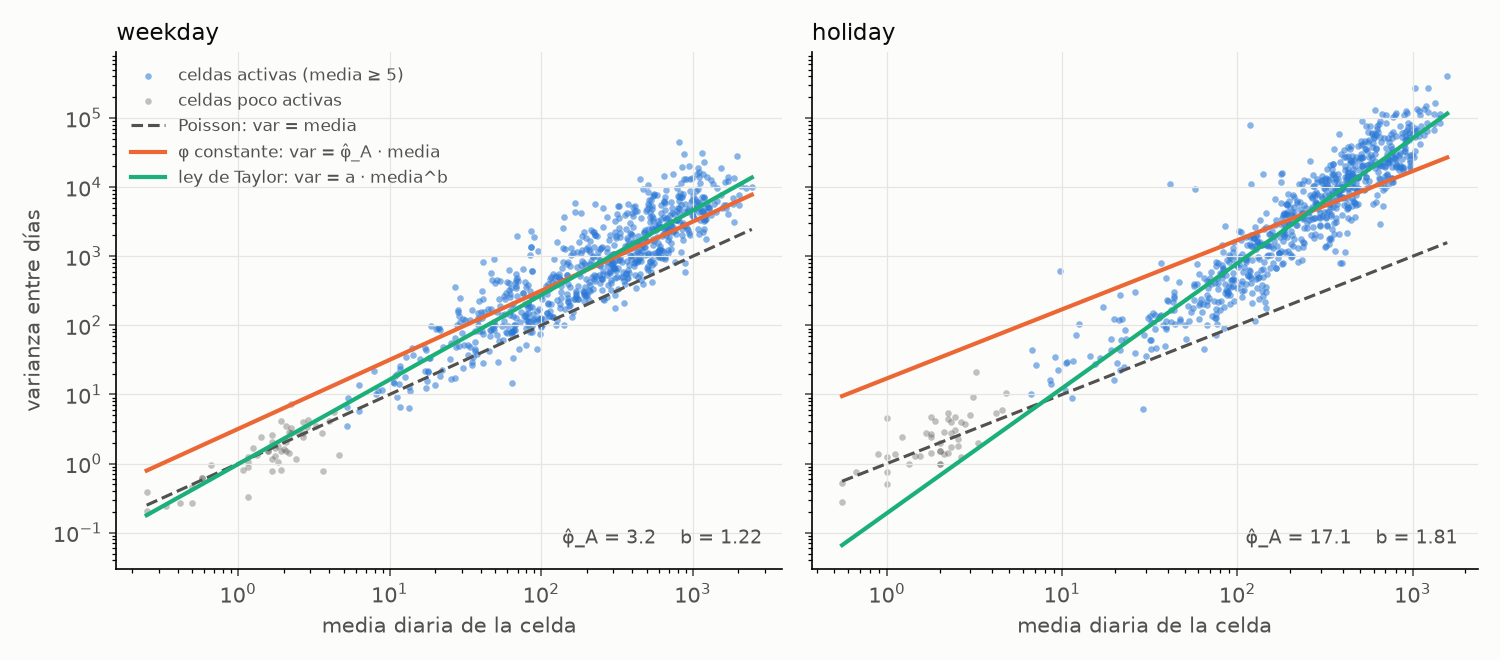
\includegraphics[width=\textwidth]{figs/Chap3/sobredispersion_media_varianza.png}
\caption{Varianza entre días frente a media diaria de cada celda, en escala
logarítmica. La recta discontinua es la de Poisson; la naranja, un modelo
cuasi-Poisson con $\varphi$ constante; la verde, la ley de potencia
$\mathrm{var} = a\,\mu^b$ ajustada a las celdas activas.}
\label{fig:prop-dispersion}
\end{figure}

\begin{enumerate}
  \item \textbf{La sobredispersión es sustancial.} La varianza de una celda
  típica es 3 veces su media en el periodo laborable y 17 veces en el feriado.
  Con la nula de Poisson, la prueba rechazaría la independencia por esta sola
  razón.
  \item \textbf{No es constante y crece con el volumen.} En escala logarítmica,
  la varianza crece con pendiente $b > 1$, y el cociente var/media pasa de 2.8 en
  las celdas poco activas a 49 en las más activas del periodo feriado. Un modelo
  cuasi-Poisson con un único $\hat\varphi$ corregiría de más los bloques poco
  activos y de menos los de mucho volumen, que son los que concentran la masa. Con
$\hat\varphi = 17.1$, la mediana del feriado, una celda poco activa con cociente
2.8 se corregiría de más unas seis veces, y una muy activa con cociente 49.1 se
corregiría de menos casi tres veces.
  \item \textbf{Una parte no afecta a la prueba, y otra es correlacionada.} Si
  la intensidad de un día se multiplica por un factor común a toda la ciudad, a
  una región o a un intervalo, por ejemplo $\mu_{dij} = a_i\, b_j\,
  \gamma_{di}$, la suma sobre los días
  $\sum_d \mu_{dij} = a_i \bigl(\sum_d \gamma_{di}\bigr) b_j$ sigue siendo un
  producto de un efecto de fila y uno de columna, y la independencia dentro del
  bloque se conserva. Por ejemplo, con $a=(1,2)$ y $b=(10,20)$, si en el día 1 el
factor es $\gamma_{1i}=(1,1)$ y en el día 2 es $\gamma_{2i}=(2,0.5)$, de modo que
la primera región está muy activa y la segunda poco, la suma sobre los dos días da
$(30,60)$ para la primera región y $(30,60)$ para la segunda, filas proporcionales
y, por tanto, ningún patrón falso. El caso $\gamma_{dj}$ es simétrico. Al eliminar esos
  efectos con el modelo log-lineal sin interacción triple, con términos
  día--región, día--intervalo y región--intervalo, la dispersión residual baja a
  2.1 y 6.7, y sigue creciendo con el volumen. Lo que queda proviene de la
  variación propia de cada celda y de la combinación de efectos
  día--región y día--intervalo, que produce desviaciones correlacionadas entre
  las celdas de un bloque, con la forma de una interacción, cuyo peso en
  $G^2_B$ crece con la masa del bloque.
\end{enumerate}

El tercer hecho tiene una consecuencia de diseño, a saber, que una nula que trate cada celda
por separado, aunque use una función de varianza que crezca con la media
(Sección~\ref{sec:est-efecto}), no puede reproducir esas desviaciones
correlacionadas. La nula de AST-CC se construye, por eso, con los días
completos, de modo que cada réplica conserva la correlación que existe entre las
celdas de un mismo día, y esa es la propiedad que justifica el procedimiento que
se describe a continuación.

\subsection{Distribución nula mediante \emph{bootstrap} de días}\label{sec:prop-bootstrap}

Todas las pruebas se calibran por simulación, de modo que se generan $B_{\mathrm{perm}}$
tablas nulas del bloque, se calcula en cada una el estadístico $t_b$ y, con el
estadístico observado $t_{\mathrm{obs}}$, el p-valor es
\begin{equation}\label{eq:prop-pval}
  p = \frac{1 + \#\{b : t_b \ge t_{\mathrm{obs}}\}}{1 + B_{\mathrm{perm}}},
\end{equation}
que incluye la tabla observada entre las réplicas y nunca vale cero
\cite{Phipson2010}. Con $B_{\mathrm{perm}}=199$ y cuatro réplicas por encima del
valor observado, el p-valor es $5/200 = 0.025$, y si ninguna lo supera es
$1/200 = 0.005$, que es el mínimo que esa cantidad de réplicas permite alcanzar.

Las réplicas se generan con los propios días observados, aplicando el principio
del \emph{bootstrap} bajo la hipótesis nula (Sección~\ref{sec:est-bootstrap}), de modo
que se remuestrean los días, pero alrededor de la media de independencia del bloque y
no de los datos observados. Para cada celda del
bloque con media diaria $\bar X_{ij}\ge 0.5$ se define la fluctuación
multiplicativa del día $d$, $F_{dij} = X_{dij}/\bar X_{ij}$, y su versión
corregida por muestra pequeña
\begin{equation}\label{eq:prop-fluctuacion}
  \tilde F_{dij} = \max\Bigl\{0,\ 1 + \sqrt{\tfrac{D}{D-1}}\,\bigl(F_{dij}-1\bigr)\Bigr\},
\end{equation}
que compensa que la varianza empírica de $D$ días subestima la poblacional. Si
el recorte en cero actúa, las $\tilde F_{dij}$ de la celda se reescalan para que
su media vuelva a ser uno. En las celdas con menos actividad el cociente no es
fiable: se toma $\tilde F_{dij}=1$ y la réplica de la celda se sortea como
Poisson con la media que le corresponde, de modo que conserve al menos esa
variabilidad. Para una celda con
cuatro días de conteos $(80,100,90,130)$ y media 100, las fluctuaciones son
$(0.8,1.0,0.9,1.3)$ y, con el factor $\sqrt{4/3}\approx1.155$, las corregidas son
$(0.77,1.00,0.88,1.35)$, que multiplican por $4/3$ la varianza de las
fluctuaciones. Cada réplica sortea
$D$ días $d_1,\dots,d_D$ con reemplazo y toma
\begin{equation}\label{eq:prop-bootstrap}
  O^{(b)}_{ij} = \frac{E^B_{ij}}{D}\sum_{k=1}^{D} \tilde F_{d_k ij},
\end{equation}
redondeado a un entero de forma estocástica, sin sesgo. En la celda anterior, si
$E^B_{ij}=400$ y se sortean los días $(4,1,4,2)$, la suma de las fluctuaciones
corregidas es $4.46$ y la réplica vale $400/4\cdot4.46\approx446$. La media de las réplicas
es la de independencia en el bloque, $E^B$, así que cumplen el nulo. Si un día
solo difiere de los demás por un factor común a todo el bloque, a una región o
a un intervalo, la fluctuación es de rango uno y la réplica sigue siendo
independiente, como exige el tercer hecho de la sección anterior; la combinación
de efectos y la variación propia de cada celda, en cambio, se trasladan tal como
aparecen en los datos. El método no supone ninguna forma para la varianza ni
para la correlación entre celdas, pero sí que los días son independientes y que
$E^B$ estima bien las medias. Además del p-valor, las réplicas proporcionan la
media $\bar t_0$ del estadístico bajo el nulo, que se usa para corregir el sesgo
del tamaño de efecto (Sección~\ref{sec:prop-parada}) sin costo adicional.

\paragraph{Evidencia preliminar de calibración.} Para elegir esta nula se
compararon varias alternativas sobre datos nulos semirreales, que consisten, para cada bloque
base de ST-CC, en 300 réplicas generadas con \eqref{eq:prop-bootstrap} a partir de
los días reales, las cuales cumplen la independencia por construcción pero tienen la
variabilidad de los datos. Cada prueba se aplicó solo con los $D$ días de cada
réplica y con 199 réplicas propias. La Tabla~\ref{tab:prop-calibracion} resume
el error de tipo~I resultante al nivel 0.05.

\begin{table}[t]
\centering
\small
\begin{tabular}{@{}lcccc@{}}
\toprule
 & \multicolumn{2}{c}{Laborable (24 bloques)} & \multicolumn{2}{c}{Feriado (24 bloques)} \\
\cmidrule(lr){2-3}\cmidrule(l){4-5}
Nula & Media & Máximo & Media & Máximo \\
\midrule
Poisson (Patefield) & 0.40 & 0.84 & 0.76 & 1.00 \\
Cuasi-Poisson, $\hat\varphi$ constante & 0.03 & 0.19 & 0.01 & 0.06 \\
Gamma--Poisson con $\mathrm{var} = a\,\mu^b$ & 0.02 & 0.11 & 0.06 & 0.42 \\
\emph{Bootstrap} de días, sin corrección & 0.06 & 0.14 & 0.11 & 0.39 \\
\emph{Bootstrap} de días \eqref{eq:prop-bootstrap} & 0.04 & 0.13 & 0.09 & 0.33 \\
\bottomrule
\end{tabular}
\caption{Error de tipo~I de la prueba ómnibus al nivel 0.05 sobre datos nulos
semirreales construidos con los días de noviembre de 2017. Para cada bloque base
de ST-CC se usaron 300 réplicas; el error de Monte Carlo por bloque es de
aproximadamente 0.013.}
\label{tab:prop-calibracion}
\end{table}

La nula de Poisson rechaza la independencia verdadera en el 40\,\% de los casos
en el periodo laborable y en el 76\,\% en el feriado. Las nulas que tratan las
celdas por separado son conservadoras en la mayoría de los bloques, lo que cuesta
potencia, y liberales en los de más volumen. El \emph{bootstrap} de días con la
corrección \eqref{eq:prop-fluctuacion} es el único cuyo error se centra en el
nominal en el periodo laborable, con media 0.044 y mediana 0.042.

En el periodo feriado, el generador de la tabla mezcla al azar sábados, domingos
y el Día de Acción de Gracias, mientras que la matriz real tiene siempre la
misma composición. Con un generador que la respeta, el error medio del \emph{bootstrap}
baja a 0.045, aunque 5 de los 24 bloques, casi todos nocturnos y de dos
intervalos, siguen por encima del nominal, con un máximo de 0.30. Remuestrear los
días dentro de cada tipo de día no lo mejora, ya que con solo cuatro sábados y cuatro
domingos, el error medio sube a 0.11. AST-CC usa, por tanto, el \emph{bootstrap} sin
estratos en ambos periodos, y la liberalidad residual en los bloques nocturnos
del periodo feriado se trata como una limitación conocida
(Sección~\ref{sec:prop-limitaciones}). Como estos datos nulos semirreales
comparten su mecanismo con el \emph{bootstrap}, lo que puede favorecerlo, la
calibración del método completo se medirá también con datos sintéticos de
mecanismo distinto (Capítulo~\ref{chap:resultados}).

\subsection{Corrección por la búsqueda del mejor corte}\label{sec:prop-minP}

El corte que se prueba fue elegido porque maximiza la separación. Si su
estadístico se comparara con la distribución $\chi^2$ de un corte fijado de
antemano, el p-valor estaría fuertemente sesgado hacia cero. Con siete candidatos
independientes de un grado de libertad, por ejemplo, la probabilidad de que al
menos uno supere el umbral del 5\,\% es $1-0.95^7\approx 0.30$, y no 0.05; los
candidatos reales están correlacionados, por lo que el sesgo es menor, pero con
las 2047 biparticiones de columnas sigue siendo grande. Este es el
problema de doble uso de los datos que \cite{Gao2024} documentan para el
agrupamiento jerárquico.

AST-CC lo corrige con un ajuste de tipo \emph{min-P} \cite{Westfall1993}, que
consiste en que en cada réplica nula se repite la búsqueda completa del mejor corte y se
registra su estadístico máximo. El p-valor \eqref{eq:prop-pval} compara así el
máximo observado con la distribución del máximo bajo el nulo, lo que ajusta a
la vez por el número de candidatos y por la correlación entre ellos, con más
potencia que una corrección de Bonferroni sobre todos los candidatos. Omitir la
repetición de la búsqueda invalida el p-valor, como lo muestra una comprobación
preliminar con bloques nulos de los tamaños de los bloques base, en la que comparar
el mejor corte de
filas con la $\chi^2$ de un corte fijo produjo errores de tipo~I de hasta 0.98
al nivel 0.05, mientras que con el ajuste \emph{min-P} el error medio fue 0.053.
Las pruebas dirigidas reutilizan las réplicas que ya generó la prueba ómnibus, y
sobre cada una se repiten las tres búsquedas. Cada prueba sigue siendo válida
por separado, y el costo de generar réplicas se paga una sola vez por bloque.

\subsection{Alcance de la corrección}

La repetición de la búsqueda corrige la selección del corte dentro de un nodo,
pero no la selección del propio nodo. Los bloques base provienen de BBAC$_I$ y
los bloques hijos provienen de cortes elegidos con los mismos datos. Esto importa porque BBAC$_I$ elige la partición base de modo que sus grupos sean
lo más distintos posible entre sí, de manera que los bloques resultantes tienden a
parecer heterogéneos aunque los datos no tengan estructura, y algo análogo ocurre
con cada corte aceptado, que se eligió por separar bien los datos que luego se
usan para probarlo. Por eso,
la validez de las pruebas en los nodos no puede darse por supuesta aunque cada
prueba individual esté bien calibrada, y el
Capítulo~\ref{chap:resultados} incluye un experimento de calibración sobre datos
nulos que mide cuántos refinamientos espurios produce el método completo al
nivel nominal, con la partición base estimada a partir de los mismos datos.

\section{Control de comparaciones múltiples}\label{sec:prop-multiplicidad}

Un árbol de refinamiento implica muchas pruebas, a saber, una por cada bloque base
y, en cascada, una por cada hijo. Aplicar el mismo nivel $\alpha$ a todas ellas
produciría muchos falsos refinamientos, y dividir $\alpha$ entre el número total
de pruebas, como hace SigTree con la corrección de Bonferroni \cite{Hu2025},
ignora la estructura jerárquica y resulta demasiado conservador. Con veinte
pruebas independientes al 5\,\%, la probabilidad de al menos un falso rechazo es
$1-0.95^{20}\approx 64$\,\%, y Bonferroni la evita dando a todas el mismo nivel
$0.05/20 = 0.0025$ aunque unos bloques tengan muchos más datos que otros.

AST-CC reparte el nivel global $\alpha$ de arriba abajo, en proporción a la masa
de cada bloque, siguiendo la lógica de las pruebas jerárquicas de
\cite{Meinshausen2008} y de \cite{Kimes2017},
\begin{equation}\label{eq:prop-alpha}
  \alpha_{B_{gh}} = \alpha\,\frac{N_{B_{gh}}}{N}\quad\text{(bloques base)},
  \qquad
  \alpha_{C} = \alpha_B\,\frac{N_C}{N_B}\quad\text{(hijos } C\in\mathcal{C}(B,s_B)\text{)},
\end{equation}
y un bloque solo se prueba si su padre fue refinado. El reparto por masa da
prioridad automática a los bloques con más datos, y los niveles de los bloques
que nunca se visitan no se gastan. Con $N=10\,000$ viajes, $\alpha=0.05$ y cuatro
bloques base de 4000, 3000, 2000 y 1000 viajes, los niveles son 0.020, 0.015, 0.010
y 0.005, que suman 0.05. Si el bloque de 4000 se corta en hijos de 3000 y 1000
viajes, estos reciben 0.015 y 0.005, que suman lo que tenía el padre. El bloque
grande trabaja entonces con 0.02, ocho veces el nivel de 0.0025 de Bonferroni, lo
que es razonable porque tiene más datos y más potencia.

El argumento de control es el siguiente. Si el nulo de independencia se cumple
en un bloque, se cumple en todos sus sub-bloques, así que los nulos verdaderos
forman subárboles completos. Un falso rechazo ocurre por primera vez en la raíz
de alguno de esos subárboles, y esas raíces son bloques disjuntos cuyos niveles
suman como máximo $\alpha$. En el ejemplo anterior, si los bloques de 2000 y 1000
viajes fueran verdaderamente nulos, la probabilidad de refinarlos por error sería a
lo sumo $0.010+0.005=0.015\le 0.05$. Si cada prueba fuera válida a su nivel y la
jerarquía estuviera fijada de antemano, la tasa de error por familia (FWER), que es
la probabilidad de al menos un falso refinamiento en todo el árbol, sería, por lo
tanto, a lo sumo $\alpha$. Como la jerarquía se construye con los
datos, la garantía es aproximada, y su comportamiento real es parte del
experimento de calibración mencionado en la sección anterior.

El reparto \eqref{eq:prop-alpha} tiene una consecuencia práctica, ya que el nivel de un
bloque pequeño puede ser inferior a la resolución $1/(B_{\mathrm{perm}}+1)$ de
un p-valor por simulación. Por eso el número de réplicas se adapta a cada
bloque, $B_{\mathrm{perm}}(B) = \max\{B_{\min},\ \lceil c/\alpha_B\rceil\}$,
acotado por un máximo $B_{\max}$ que limita el costo. Con los valores de
referencia, un bloque con $\alpha_B=0.02$ usa 199 réplicas, uno con $\alpha_B=0.005$
usa 400 y uno con $\alpha_B=0.0001$ llega al máximo de 20\,000. Si incluso con $B_{\max}$
réplicas el p-valor mínimo $1/(B_{\max}+1)$ supera $\alpha_B$, el bloque no
puede rechazarse y se marca como hoja inalcanzable, para distinguirla de
una hoja homogénea. Además se aplica la parada secuencial de \cite{Besag1991},
en la que la simulación se detiene en cuanto se acumulan $h$ réplicas con estadístico
mayor o igual que el observado. Las réplicas se generan por lotes de 500 y la regla se
evalúa al cierre de cada lote, de modo que el p-valor es la proporción de réplicas que
igualan o superan al observado en las generadas hasta ese momento. Con
$B_{\mathrm{perm}}\le 500$ la regla no se activa y se usan todas las réplicas, lo que
es barato porque la prueba ómnibus solo requiere calcular $G^2$ sobre cada tabla;
el ahorro está en los bloques con $\alpha_B$ muy pequeño, que exigen miles de
réplicas, donde un bloque claramente no significativo se abandona tras el primer
lote. Si el bloque supera la prueba ómnibus, la simulación se completó
y sus réplicas sirven para las pruebas dirigidas.

\section{Criterios de parada}\label{sec:prop-parada}

Con matrices de millones de viajes, casi cualquier desviación de la
independencia resulta significativa. Los propios \cite{Hu2025} señalan que el
estadístico $\chi^2$ crece con el tamaño de la muestra y dificulta el control de
los falsos descubrimientos. Por eso AST-CC exige la significancia y un
tamaño de efecto mínimo, nunca solo una de las dos. Un bloque con un millón de
viajes e información mutua de 0.0005 nats por observación tiene $G^2 = 1000$, un
p-valor prácticamente nulo, y una interacción irrelevante; otro con mil viajes e
información mutua de 0.05 tiene $G^2=100$, y si pasa la prueba también supera el
umbral de efecto. La significancia crece con el número de viajes y el tamaño de
efecto no. La Tabla~\ref{tab:prop-parada} reúne todos los criterios.

\begin{table}[t]
\centering
\small
\begin{tabular}{>{\raggedright\arraybackslash}p{0.2\textwidth}>{\raggedright\arraybackslash}p{0.3\textwidth}>{\raggedright\arraybackslash}p{0.4\textwidth}}
\toprule
Criterio & Condición para ser hoja & Justificación \\
\midrule
Tamaño mínimo & $|I|<2$ o $|J|<2$ & Con una sola fila o columna, $G^2_B=0$, de modo que no hay interacción posible. \\
Masa mínima & $N_B<N_{\min}$ & Evita probar bloques con muy poca actividad. \\
Profundidad máxima & $d\ge d_{\max}$ & Acota el costo y la complejidad del árbol. \\
Nivel inalcanzable & $1/(B_{\max}+1)>\alpha_B$ & Con el máximo de réplicas, la prueba no podría rechazar. \\
Significancia & $p_{\mathrm{omn}}>\alpha_B$, o ningún corte con p-valor $\le\alpha_B$ & No hay evidencia de heterogeneidad, o no puede localizarse. \\
Tamaño de efecto & $\tilde I_B<\delta$ & La interacción residual es irrelevante aunque sea detectable. \\
Ganancia del corte & $\tilde g_{B,s}<\delta$ & El corte explica demasiado poca información. \\
\bottomrule
\end{tabular}
\caption{Criterios de parada de AST-CC. Los cuatro primeros son reglas que no
dependen de la estructura interna del bloque, análogas a las de SigTree \cite{Hu2025}; los
tres últimos son estadísticos.}
\label{tab:prop-parada}
\end{table}

El umbral $\delta$ es la defensa principal contra la inflación por tamaño de
muestra. Tiene una interpretación directa, información mutua en nats por
observación, y no crece con $N$. En los datos de esta tesis es, además, el que
decide el refinamiento en los primeros niveles del árbol, ya que con masas de unos mil
a cientos de miles de viajes por bloque, el cociente $G^2_B/\nu_B$ de los
bloques base de ST-CC va de 3 a más de 1700, y la prueba de independencia
rechaza en prácticamente todos ellos. La prueba cobra importancia en los bloques
pequeños y profundos, donde la masa es menor.

\paragraph{Tamaño de efecto corregido por sesgo.} La información mutua empírica
está sesgada hacia arriba en los bloques pequeños
(Sección~\ref{sec:est-efecto}). Aunque no haya interacción,
$\mathrm{E}[G^2_B]\approx\nu_B = (|I|-1)(|J|-1)$ bajo Poisson, y más con
sobredispersión, de modo que $\mathrm{E}[\hat I_B]\approx \nu_B/(2N_B) > 0$. En el
periodo laborable, por ejemplo, un bloque de 1033 viajes y 12 grados de
libertad tiene $\hat I_B = 0.017$, el quinto valor más alto de los 24 bloques,
y cerca de un tercio de esa cantidad ($12/2066\approx 0.006$) es la que se
esperaría solo por el ruido de Poisson. Si además la media de $G^2$ bajo el nulo
fuera, por la sobredispersión, de unas 25 unidades en lugar de 12, el mismo
bloque tendría un tamaño de efecto corregido de $(35.1-25)/2066\approx 0.005$, lo
que muestra cuánto depende la lectura del ruido que se descuente; el valor de 25 es
ilustrativo. AST-CC usa, por eso, las versiones
corregidas
\begin{equation}\label{eq:prop-efecto-corregido}
  \tilde I_B = \max\Bigl\{0,\ \frac{G^2_B - \bar t_0}{2N_B}\Bigr\},
  \qquad
  \tilde g_{B,s} = \max\Bigl\{0,\ \frac{G^2_{B,s} - \bar t_{0,s}}{2N_B}\Bigr\},
\end{equation}
donde $\bar t_0$ es la media de $G^2_B$ sobre las réplicas nulas de la prueba
ómnibus y $\bar t_{0,s}$ la media del estadístico dirigido
\eqref{eq:prop-dirigidos} sobre las mismas réplicas. Ambas medias se obtienen de
réplicas que ya se generan para los p-valores, así que la corrección no tiene
costo. Como las réplicas siguen el \emph{bootstrap} de días, $\bar t_0$ incorpora la
variabilidad real entre días; y como $\bar t_{0,s}$ se calcula repitiendo la
búsqueda, descuenta también el optimismo de elegir el mejor corte.

\paragraph{Elección de $\delta$.} Su valor no se fija a priori. Como referencia
de escala, la información mutua $\hat I_B$ de los bloques base de ST-CC va de
0.0012 a 0.061 nats en el periodo laborable y de 0.0017 a 0.19 en el feriado.
En el Capítulo~\ref{chap:resultados} se recorre una rejilla que cubre ese rango,
por ejemplo $\delta\in\{0.001, 0.0025, 0.005, 0.01, 0.02\}$, y para cada valor
se reportan el número de hojas, la fracción del término de interacción local de
ST-CC que explica el árbol según el Corolario~\ref{cor:stcc},
$\sum_{B\in\mathcal{S}}G^2_{B,s_B}\big/\sum_{g,h}G^2_{gh}$, y la estabilidad de
las hojas. Como medida estandarizada complementaria puede reportarse la $V$ de
Cramér de cada hoja.

\section{Algoritmo}\label{sec:prop-algoritmo}

Los Algoritmos~\ref{alg:astcc} y \ref{alg:mejorcorte} reúnen los elementos
anteriores. La Tabla~\ref{tab:prop-parametros} resume los parámetros del método,
junto con los valores de referencia que se usarán en los experimentos y que se
someterán a un análisis de sensibilidad, como se indica en su última columna. El
Algoritmo~\ref{alg:astcc} describe el procedimiento recursivo completo, desde la
partición base hasta la decisión sobre cada bloque, y el
Algoritmo~\ref{alg:mejorcorte} detalla cómo se selecciona el mejor corte y se
calcula su p-valor con el ajuste \emph{min-P}.

\begin{algorithm}[t]
\caption{Refinamiento jerárquico de ST-CC con AST-CC}\label{alg:astcc}
\begin{algorithmic}[1]
\Require Matriz de conteos $O\in\mathbb{N}^{m\times n}$ y sus días $X_1,\dots,X_D$; $K_R$, $K_T$; nivel $\alpha$; umbral $\delta$; $N_{\min}$, $d_{\max}$; y los demás parámetros de la Tabla~\ref{tab:prop-parametros}
\Ensure Árbol de refinamiento $\mathcal{T}$
\State $(\rho,\tau)\gets$ BBAC$_I(O, K_R, K_T)$ con base C5 y búsqueda local \Comment{partición base}
\ForAll{bloque base $B_{gh}$}
  \State \Call{Refinar}{$B_{gh},\ \alpha N_{B_{gh}}/N,\ 0$}
\EndFor
\State \Return $\mathcal{T}$
\Statex
\Procedure{Refinar}{$B=I\times J,\ \alpha_B,\ d$}
  \If{$|I|<2$ \textbf{o} $|J|<2$ \textbf{o} $N_B<N_{\min}$ \textbf{o} $d\ge d_{\max}$}
    \State marcar $B$ como hoja; \Return
  \EndIf
  \State $B_{\mathrm{perm}}\gets\min\{B_{\max},\ \max\{B_{\min},\ \lceil c/\alpha_B\rceil\}\}$
  \If{$1/(B_{\mathrm{perm}}+1)>\alpha_B$}
    \State marcar $B$ como hoja inalcanzable; \Return
  \EndIf
  \State calcular $G^2_B$ con \eqref{eq:prop-G2}
  \State generar réplicas $O^{(b)}$ con \eqref{eq:prop-bootstrap}, por lotes, hasta $B_{\mathrm{perm}}$ o hasta que al cierre de un lote $h$ superen $G^2_B$ \Comment{la parada solo se activa si el bloque no es significativo}
  \State $(p_{\mathrm{omn}}, \bar t_0)\gets$ p-valor y media nula de $G^2_B$ sobre las réplicas
  \State $\tilde I_B\gets\max\{0,\ (G^2_B-\bar t_0)/(2N_B)\}$
  \If{$p_{\mathrm{omn}}>\alpha_B$ \textbf{o} $\tilde I_B<\delta$}
    \State marcar $B$ como hoja homogénea; \Return
  \EndIf
  \State $(s_{\mathrm{fil}},p_{\mathrm{fil}},\bar t_{\mathrm{fil}})\gets$ \Call{MejorCorte}{$B,\ \text{filas},\ \{O^{(b)}\}$}
  \State $(s_{\mathrm{col}},p_{\mathrm{col}},\bar t_{\mathrm{col}})\gets$ \Call{MejorCorte}{$B,\ \text{columnas},\ \{O^{(b)}\}$}
  \If{$\min(p_{\mathrm{fil}},p_{\mathrm{col}})\le\alpha_B$}
    \State $s\gets$ corte de menor p-valor (desempate por $z$)
  \Else
    \State $(s_{\mathrm{conj}},p_{\mathrm{conj}},\bar t_{\mathrm{conj}})\gets$ \Call{MejorCorte}{$B,\ \text{conjunto},\ \{O^{(b)}\}$}
    \If{$p_{\mathrm{conj}}>\alpha_B$}
      \State marcar $B$ como hoja heterogénea no localizada; \Return
    \EndIf
    \State $s\gets s_{\mathrm{conj}}$
  \EndIf
  \State $\tilde g_{B,s}\gets\max\{0,\ (G^2_{B,s}-\bar t_{0,s})/(2N_B)\}$ \Comment{$\bar t_{0,s}$ es la media nula del tipo de $s$}
  \If{$\tilde g_{B,s}<\delta$}
    \State marcar $B$ como hoja heterogénea no localizada; \Return
  \EndIf
  \ForAll{$C\in\mathcal{C}(B,s)$}
    \State \Call{Refinar}{$C,\ \alpha_B N_C/N_B,\ d+1$}
  \EndFor
\EndProcedure
\end{algorithmic}
\end{algorithm}

\begin{algorithm}[t]
\caption{Selección del mejor corte con ajuste \emph{min-P}}\label{alg:mejorcorte}
\begin{algorithmic}[1]
\Function{MejorCorte}{$B,\ \text{tipo},\ \{O^{(b)}\}_{b=1}^{B_{\mathrm{perm}}}$}
  \State $s^\ast\gets$ \Call{Buscar}{$O|_B,\ \text{tipo}$} \Comment{Sección~\ref{sec:prop-candidatos}}
  \State $t_{\mathrm{obs}}\gets G^2_{B,s^\ast}$
  \For{$b=1,\dots,B_{\mathrm{perm}}$}
    \State $s_b\gets$ \Call{Buscar}{$O^{(b)},\ \text{tipo}$} \Comment{se repite la búsqueda completa}
    \State $t_b\gets G^2_{B,s_b}$ calculado sobre $O^{(b)}$
  \EndFor
  \State $p\gets \bigl(1+\#\{b: t_b\ge t_{\mathrm{obs}}\}\bigr)/\bigl(1+B_{\mathrm{perm}}\bigr)$
  \State $\bar t\gets$ media de los $t_b$ \Comment{para \eqref{eq:prop-efecto-corregido}}
  \State \Return $(s^\ast, p, \bar t)$
\EndFunction
\end{algorithmic}
\end{algorithm}

\begin{table}[t]
\centering
\small
\begin{tabular}{>{\raggedright\arraybackslash}p{0.18\textwidth}>{\raggedright\arraybackslash}p{0.4\textwidth}>{\raggedright\arraybackslash}p{0.32\textwidth}}
\toprule
Parámetro & Papel & Valor de referencia \\
\midrule
$K_R$, $K_T$ & Resolución inicial de la partición base & Los de \cite{Liu2021}; sensibilidad en el Cap.~\ref{chap:resultados} \\
Inicializaciones de BBAC$_I$ & Ejecuciones de la partición base, cada una con búsqueda local & $200$, como \cite{Liu2021} \\
$\alpha$ & Nivel global (FWER sobre el árbol) & $0.05$ \\
$\delta$ & Información mutua mínima por observación, corregida por sesgo & Rejilla en $[0.001, 0.02]$ nats; sensibilidad \\
$N_{\min}$, $d_{\max}$ & Reglas triviales de parada & $500$ viajes y profundidad $6$; sensibilidad \\
$B_{\min}$, $c$, $B_{\max}$ & Réplicas mínimas, resolución respecto de $\alpha_B$ y máximo & $199$, $2$ y $20\,000$ \\
$h$ & Parada secuencial de Besag y Clifford, evaluada por lotes de 500 réplicas & $10$ \\
Límites de enumeración & Tamaño máximo para buscar cortes por enumeración & $|I|\le14$; $|J|\le6$ en el corte conjunto \\
$R_{\mathrm{ini}}$ & Inicializaciones del 2-medias para bloques con más de 14 filas & $10$ \\
$\kappa$ & Índice de Jaccard mínimo para la frecuencia de soporte & $0.5$ como punto de partida \\
\bottomrule
\end{tabular}
\caption{Parámetros de AST-CC.}
\label{tab:prop-parametros}
\end{table}

Los parámetros de la tabla son de dos tipos. Los que condicionan el resultado y
por eso se someten a análisis de sensibilidad son $K_R$, $K_T$, $\alpha$, $\delta$,
$N_{\min}$ y $d_{\max}$, que son decisiones del investigador. Los demás
(inicializaciones, número de réplicas, parada secuencial y límites de enumeración)
son técnicos y buscan dar fiabilidad a las pruebas sin ser el foco de la
interpretación. Un recorrido del Algoritmo~\ref{alg:astcc} con números ayuda a
verlo. Sea $N=10\,000$, $\alpha=0.05$ y un bloque base de 4000 viajes, con nivel
$\alpha_B=0.02$. El bloque supera las reglas triviales y su número de réplicas es
$\min\{20\,000,\max\{199,\lceil 2/0.02\rceil\}\}=199$, con un p-valor mínimo de
$1/200=0.005\le 0.02$, de modo que la prueba es alcanzable. Si la prueba ómnibus da
$p_{\mathrm{omn}}=0.005$ y $\tilde I_B=0.03\ge\delta=0.005$, el bloque pasa la
puerta. Si además $p_{\mathrm{fil}}=0.005$ y $p_{\mathrm{col}}=0.4$, solo el corte de
filas es significativo y se acepta cuando su ganancia corregida supera $\delta$. Si
deja hijos de 3000 y 1000 viajes, estos reciben niveles de 0.015 y 0.005, y el segundo
usa $\max\{199,400\}=400$ réplicas antes de repetir el mismo procedimiento. El
criterio de nivel inalcanzable de la Tabla~\ref{tab:prop-parada} usa $B_{\max}$ y el
algoritmo usa $B_{\mathrm{perm}}$, que está acotado por $B_{\max}$; ambos coinciden,
porque si $\alpha_B$ es grande la prueba es alcanzable y si es pequeño
$B_{\mathrm{perm}}$ llega a $B_{\max}$.

\subsection{Costo computacional}

La partición base cuesta lo mismo que ST-CC, $O(mn(K_R+K_T))$ por iteración de
BBAC$_I$ y por inicialización, más la búsqueda local; esta última puede evaluar
cada movimiento de una fila o columna en $O(K_R K_T)$, porque con las bases C2 y
C5 la divergencia depende solo de los totales de bloque. El costo adicional se
concentra en las pruebas por simulación. En un bloque $B=I\times J$, cada
réplica requiere generar una tabla de $|I|\times|J|$ y repetir las búsquedas. La
de columnas evalúa $2^{|J|-1}-1$ tablas colapsadas de $|I|\times2$, y la de
filas, mientras $|I|\le 14$, $2^{|I|-1}-1$ tablas de $2\times|J|$. El costo por
bloque es del orden de
\[
  O\Bigl(B_{\mathrm{perm}}(B)\,\bigl[\,2^{|J|}|I| + 2^{\min(|I|,14)}|J|\,\bigr]\Bigr),
\]
más el del corte conjunto, que solo se evalúa cuando ningún corte
unidimensional es significativo. Con $n=12$ y bloques base de a lo sumo quince
filas, los dos términos exponenciales están acotados por constantes moderadas. Un
bloque de 10 filas y 12 columnas requiere del orden de $2^{12}\cdot10+2^{10}\cdot12
\approx 5\cdot10^4$ operaciones elementales por réplica, y uno de 14 filas, unas
$2.5\cdot10^5$, de modo que con 199 réplicas el trabajo es del orden de $10^7$ y
$5\cdot10^7$ operaciones respectivamente. Estas cifras son órdenes de magnitud y
no tiempos medidos, que se reportarán junto con los resultados del
Capítulo~\ref{chap:resultados}.
Tres propiedades mantienen el costo total manejable. La primera es que la parada
secuencial abandona pronto los bloques no significativos; la segunda, que los
bloques de un mismo nivel son independientes dado el árbol, por lo que se
procesan en paralelo; y la tercera, que el tamaño de los bloques decrece con la
profundidad.

\section{Representación e interpretación de los resultados}\label{sec:prop-representacion}

La partición de ST-CC se lee como $K_T$ patrones espaciales con su dinámica
temporal y $K_R$ patrones temporales con su distribución espacial. Con
refinamiento local, esa lectura deja de existir como objeto único, porque la
partición temporal puede cambiar de un subconjunto de regiones a otro. Para no
perder interpretabilidad, AST-CC acompaña el árbol de cinco productos.

\paragraph{Descriptores de hoja.} Para cada hoja $L = I_L\times J_L$ se reportan
sus regiones y horarios, su masa $N_L$, su interacción residual $\tilde I_L$ (solo
para las hojas que llegaron a la prueba ómnibus, pues requiere las réplicas nulas), su
tipo (homogénea, heterogénea no localizada, inalcanzable o trivial, esta última por
las reglas de tamaño, masa o profundidad de la Tabla~\ref{tab:prop-parada}) y su nivel de
actividad relativo
\begin{equation}\label{eq:prop-lift}
  \ell_L = \frac{N_L}{\sum_{(i,j)\in L} O_{i\cdot}\,O_{\cdot j}/N},
\end{equation}
que compara la actividad observada en la hoja con la que predicen los volúmenes
globales de sus regiones e intervalos. Un valor $\ell_L>1$ indica que ese grupo
de regiones se activa en ese grupo de horarios más de lo que corresponde a su
volumen, y un valor $\ell_L<1$, que está más apagado de lo que corresponde. Por
ejemplo, con $N=10\,000$ y una hoja formada por dos regiones de 500 y 300 viajes
totales y dos horarios de 1000 y 2000, el esperado es
$800\cdot3000/10\,000=240$, y si la hoja tiene 360 viajes, $\ell_L=1.5$. La referencia es el modelo de independencia de toda la matriz y no el
del bloque padre, ya que este último reproduce los totales de fila y de columna del
padre, de modo que, tras un corte de filas o de columnas, el cociente respecto
del padre vale exactamente uno en todos los hijos y no distingue nada. Un bloque
de 4000 viajes cortado en hijos de 3000 y 1000 daría $3000/3000=1$ y
$1000/1000=1$ respecto de su padre.

\paragraph{Árbol anotado.} Cada nodo interno muestra el tipo de corte, la
ganancia corregida $\tilde g_{B,s}$ y el p-valor, de modo que se lee qué parte de la
heterogeneidad fue espacial y qué parte temporal. Esta representación conserva la
trazabilidad de las decisiones, ya que cada hoja puede leerse como el resultado de
la secuencia de cortes que llevó hasta ella, de manera análoga a la lectura de las
reglas de un árbol de decisión. Si un bloque base se corta por filas y uno de
sus hijos se corta después por columnas, la hoja resultante se lee como un grupo
de regiones, dentro de ese bloque, en un grupo de horarios, donde la primera
pregunta fue espacial y la segunda temporal.

\paragraph{Matriz teselada.} La matriz se reordena según la partición base y,
dentro de cada bloque, según sus cortes, y se dibuja con los contornos de las
hojas y un color proporcional a $\ell_L$, como en la
Figura~\ref{fig:prop-teselacion}. De este modo se obtiene una vista global en la
que los patrones locales aparecen como rectángulos de color distinto dentro de
bloques que, en el tablero de ST-CC, se mostraban uniformes.

\paragraph{Mapas de profundidad.} Para cada región se representa en el mapa la
profundidad máxima que alcanza el refinamiento en sus filas, y análogamente para
cada intervalo de tiempo. Si una región aparece en hojas de profundidades 1, 3 y 2,
su valor en el mapa es 3. Estos mapas indican dónde y cuándo la partición base
resulta insuficiente. Un mapa con profundidad uniforme indicaría que el tablero de
ST-CC era suficiente, mientras que las zonas con profundidades altas señalan las
regiones y los horarios donde se concentra la interacción espacio-temporal local.

\paragraph{Frecuencia de soporte.} Como BBAC$_I$ converge a mínimos locales y
el refinamiento es voraz, cada hoja se acompaña de su frecuencia de soporte,
que es la proporción de ejecuciones, con distintas inicializaciones de la partición
base, en que aparece una hoja con índice de Jaccard, medido sobre celdas,
mayor o igual que $\kappa$ respecto de ella. El índice de Jaccard entre dos
conjuntos de celdas es el cociente entre el tamaño de su intersección y el de su
unión, y vale 1 si son idénticos y 0 si no comparten ninguna. Una hoja de $3\times2$
celdas y otra de $2\times2$ contenida en ella tienen un índice de $4/6\approx0.67$,
de modo que no se cuentan como la misma hoja con $\kappa=0.7$ y sí con
$\kappa=0.5$. Una hoja con soporte bajo, por ejemplo la que aparece en menos de la
mitad de las ejecuciones, no debe interpretarse como hallazgo.

\section{Alcance y limitaciones del diseño}\label{sec:prop-limitaciones}

Varias limitaciones se derivan directamente de las decisiones de diseño y
conviene explicitarlas antes de los experimentos, porque condicionan tanto la
interpretación de los resultados como el diseño de las comparaciones que se
presentarán en el Capítulo~\ref{chap:resultados}. Cada una se describe a
continuación junto con la forma en que se piensa evaluar su efecto.

\begin{itemize}
  \item \textbf{Restricción guillotina.} El refinamiento solo mira hacia
  dentro de cada bloque. Un patrón local que cruce la frontera entre dos
  bloques base no puede recuperarse como una sola hoja, sino como hojas
  separadas en cada bloque. Por ejemplo, un patrón en las regiones 3 a 6 en las
  mismas horas, con las regiones 3 y 4 en un bloque base y las 5 y 6 en otro, se
  recupera como dos hojas pequeñas y no como un rectángulo de cuatro regiones.
  \item \textbf{Dependencia de la partición base.} El refinamiento parte de un
  óptimo local de BBAC$_I$, cuyo paisaje tiene muchos mínimos locales; la
  búsqueda local y las múltiples inicializaciones lo atenúan, y la frecuencia
  de soporte (Sección~\ref{sec:prop-representacion}) mide su efecto sobre las
  hojas. La elección de la base también importa, ya que con C5 y con C2 se obtienen
  tableros muy distintos, y C5 deja menos interacción local por refinar, porque
  agrupa las regiones por la forma de su perfil y no por su volumen.
  \item \textbf{Resolución de entrada.} Los cortes agrupan regiones e
  intervalos, pero no los subdividen, de modo que el método no puede bajar de la resolución
  espacial y temporal de la matriz. Los resultados dependen, por tanto, de la
  zonificación usada, que en el caso de las zonas de taxi de Nueva York tiene
  tamaños muy dispares.
  \item \textbf{Parámetros.} El método no elimina $K_R$ y $K_T$, sino que
  cambia su papel, pues fijan la resolución inicial, mientras que la resolución
  final la deciden $\alpha$ y $\delta$, dos parámetros con interpretación
  directa. Esta afirmación solo se sostiene si el resultado final es
  razonablemente estable frente a $K_R$ y $K_T$, lo que debe comprobarse
  empíricamente.
  \item \textbf{Comparación con rejillas más finas.} Cabe preguntar por qué
  no basta con aumentar $K_R$ y $K_T$ o elegirlos con Cross-Associations
  \cite{Chakrabarti2004}. La respuesta debe ser empírica, y consiste en comprobar que una rejilla global con
  el mismo número de parámetros, o con el mismo valor de \eqref{eq:prop-bic},
  no recupera los patrones locales que encuentra AST-CC. La diferencia en el
  número de parámetros ilustra el argumento. Con $n=12$ intervalos repartidos en
  $K_T=4$ grupos de tres columnas, un corte de filas en un único bloque añade
  $|J|-1=2$ parámetros, mientras que partir globalmente el mismo grupo de filas a
  lo largo de los cuatro grupos de columnas añade $4\cdot2=8$.
  \item \textbf{Validez de las pruebas.} La selección de los nodos a partir de
  los datos puede inflar el error de tipo~I. El \emph{bootstrap} de días supone que
  los días son independientes y usa $E^B$ como estimación de las medias; con
  pocos días, como en el periodo feriado, es algo liberal en los bloques
  nocturnos. Por eso es indispensable un experimento de calibración sobre datos
  nulos.
  \item \textbf{Costo frente a resolución.} El reparto del nivel por masa hace
  que los bloques con muy pocos viajes reciban niveles menores que la
  resolución alcanzable con $B_{\max}$ réplicas. Esos bloques quedan como hojas
  inalcanzables, ya que el método no afirma que sean homogéneos, sino que no puede
  probarlos al nivel asignado. Con $N=10^6$ y $\alpha=0.05$, por ejemplo, un
  bloque de 600 viajes recibe $\alpha_B=3\cdot10^{-5}$; supera el mínimo de masa,
  pero el p-valor más pequeño que alcanza con 20\,000 réplicas es
  $1/20\,001\approx5\cdot10^{-5}$, mayor que su nivel.
  \item \textbf{Significativo no es interesante.} Una hoja puede tener
  heterogeneidad detectable y ser irrelevante en el dominio. Por eso se reporta
  siempre el tamaño de efecto junto al p-valor, y los patrones principales se
  contrastan con conocimiento del dominio, como el foco alrededor de Penn
  Station que identifican \cite{Liu2021}.
\end{itemize}

\paragraph{Extensiones que quedan como trabajo futuro.} Varias alternativas se
consideraron durante el diseño y quedan fuera del alcance de esta tesis.
Entre ellas se encuentra el control jerárquico de la tasa de falsos descubrimientos de
\cite{Yekutieli2008}, más permisivo que la FWER cuando se esperan muchos
refinamientos, que se dejó fuera porque la FWER es la garantía más simple de
interpretar en una primera versión del método. Otra es una variante que elija la
partición y los cortes con la mitad de los días y los pruebe con la otra mitad, lo
que elimina el doble uso de los datos a costa de potencia, en la línea del
\emph{count splitting} de \cite{Neufeld2024cs}, y que exige antes comprobar que la
mitad de los días basta para estimar la partición. También se consideraron nulas
paramétricas con una función de varianza por celda, como la ley de potencia de
\cite{Taylor1961}, que no se adoptaron porque, como muestra la
Sección~\ref{sec:prop-calibracion}, no reproducen las desviaciones correlacionadas
entre las celdas de un bloque. Los cortes de columnas podrían restringirse a
intervalos consecutivos, lo que reduciría las 2047 biparticiones posibles con doce
intervalos a solo 11 y daría patrones más fáciles de interpretar, a costa de no
capturar horarios no contiguos, como las dos horas punta del día. Por último, un
paso posterior de fusión de hojas vecinas recuperaría los patrones que cruzan
bloques base, que es la limitación de la restricción guillotina.

\section{Consideraciones Finales}\label{sec:prop-final}

Este capítulo presentó AST-CC, una extensión de ST-CC que refina localmente la
partición en tablero mediante un árbol de cortes guiados por pruebas de
hipótesis. La pieza teórica central es la
Proposición~\ref{prop:ganancia}, según la cual, bajo el modelo de independencia por hoja, la
divergencia del árbol se descompone exactamente entre las hojas y la ganancia de
cada corte es un estadístico de razón de verosimilitud. Con ella, el
Corolario~\ref{cor:stcc} muestra que el método descompone, de forma controlada,
el término de interacción local que ST-CC deja sin modelar, de modo que el
criterio de refinamiento y la función objetivo de ST-CC son la misma cantidad
vista a distintas escalas.

Sobre esa base, el método combina una prueba ómnibus calibrada con un \emph{bootstrap}
de los días observados, que reproduce su variabilidad real; pruebas dirigidas
que localizan la estructura con un ajuste \emph{min-P} que repite la búsqueda en cada
réplica; un reparto jerárquico del nivel de significancia a lo largo del árbol;
y un umbral de tamaño de efecto, corregido por sesgo, que no crece con el número
de viajes y que, a la escala de estos datos, es el que decide el refinamiento.
Las limitaciones identificadas, en particular la validez aproximada de las
pruebas cuando la jerarquía se construye con los datos, orientan directamente
el diseño experimental del Capítulo~\ref{chap:resultados}, donde el método se
evalúa sobre datos sintéticos con patrones locales conocidos, sobre datos nulos
y sobre los datos de taxis de Manhattan. Cada limitación tiene allí una forma de
evaluarse, que es la calibración sobre datos nulos para la validez de las pruebas,
la comparación con rejillas globales de igual número de parámetros para el valor del
refinamiento local, y el análisis de sensibilidad a $K_R$, $K_T$, $\alpha$ y
$\delta$ para la dependencia de la partición base y de los parámetros.
 %Inserta el capítulo 3: Propuesta
\chapter{Pruebas y Resultados}\label{chap:resultados}
 %Inserta el capítulo 4
\chapter{Conclusiones y Trabajos Futuros}\label{chap:conclusiones}

Las conclusiones de la tesis son una parte muy importante y tiene las siguientes partes.

Escribir las conclusiones de su trabajo por cada uno de los objetivos específicos definidos en el Capítulo 1 y luego escribir la conclusión general de tu trabajo.

\section{Problemas encontrados}
La segunda  parte de este capítulo corresponde a los problemas encontrados, esta sección es muy importante para que los siguientes estudiantes o investigadores que hagan algo en esta línea no cometan los mismos errores y tu tesis sea un buen peldaño para avanzar más rápido.

\section{Recomendaciones}
En esta sección el tesista debe reflejar que la tesis ha permitido adquirir nuevos conocimientos que podrían servir para guiar otros trabajos en el futuro.

\section{Trabajos futuros}
En base a los puntos anteriores es recomendable que tu tesis también sugiera trabajos futuros. Esta sección es esecialmente útil para otras ideas de tesis.

Todo este capítulo no debe ser más de unas 4 páginas. %Inserta el capítulo 5

%%%%%%%%%%%%%%%%%%%%%%%%%%%%%%%%%%%%%%%%%%%%%%%%%%%%%%%%%%%%%%%%%%%%%%

\bibliographystyle{apalike}

\bibliography{Bibliog}
\addcontentsline{toc}{chapter}{Bibliografía}
\end{document}
